\documentclass[a4paper,11pt]{article}
\usepackage{graphicx}
\usepackage[font=normal,textfont=it]{caption}
\DeclareCaptionType{Code} %Preparation for eventual code numbering
\renewcommand{\theCode}{\arabic{Code}}

\usepackage{subcaption}
%\usepackage[numbers]{natbib}
\usepackage{url}
\usepackage{array}
\usepackage{makecell}
\usepackage{comment}
\usepackage{setspace}
%\usepackage{fixltx2e}
%% Language and font encodings

\usepackage[T1]{fontenc}
\usepackage[english]{babel}
\usepackage[utf8]{inputenc}
\usepackage{libertinus} % Use font of arbitrary sizes 
                        % (removes bibliography font warning)
\usepackage{csquotes} % Removes a compilation warning
\usepackage{changepage}

\usepackage{lipsum}
\usepackage[acronym]{glossaries}

\makenoidxglossaries
\loadglsentries[acronym]{glossaries.tex}


%SI Package
\usepackage[binary-units=true]{siunitx}
%\sisetup{group-separator = \text{\,}}
%\sisetup{group-minimum-digits = {4}}

%footnote
\usepackage[bottom]{footmisc}

%% Sets page size and margins
\usepackage[a4paper,top=2cm,bottom=2cm,left=2cm,right=2cm,marginparwidth=1.75cm]{geometry}

%% Useful packages
\usepackage{amsmath}
\DeclareMathOperator{\E}{\mathbb{E}}
\usepackage{graphicx}
\usepackage{mathtools}
\usepackage{textcomp} %defines \perthousand and \micro for gensymb
\usepackage{gensymb} %math in text
\usepackage[unicode=true,pdfusetitle,
   bookmarks=true,
   bookmarksnumbered=false,
   bookmarksopen=false,
   breaklinks=false,
   pdfborder={0 0 1},
   backref=false,
   colorlinks=false]{hyperref}
%\usepackage[colorinlistoftodos]{todonotes}
%\usepackage[colorlinks=true, allcolors=black]{hyperref}

%packages for hyperlinperlin
%\usepackage{hyperref}
%\hypersetup{pdftex,colorlinks=false,allcolors=black}
%\usepackage{hypcap}

%Bibliography
\usepackage[sorting=none]{biblatex}
\addbibresource{references.bib}



\usepackage{chngcntr}
%\counterwithin{figure}{section}
\counterwithin{table}{section}

%\usepackage[table,xcdraw]{xcolor}
\usepackage{amssymb}
\usepackage{float}
\usepackage{adjustbox}
\usepackage{textgreek}
\usepackage{multirow}
\usepackage{color}
\usepackage[table,xcdraw,dvipsnames]{xcolor}
\usepackage{wrapfig}
\usepackage[final]{pdfpages}
\usepackage{listings}
\lstset{
  basicstyle=\ttfamily,
  columns=fullflexible,
}
\renewcommand{\familydefault}{\sfdefault}

\title{Inter-seasonal Performance of Gaussian Process-based
Model Predictive Control of Buildings}

\author{Radu C. Martin}

%header
%\usepackage[headsep=0.5cm,margin=1.5cm,bottom=2cm,headheight=5pt,includeheadfoot]{geometry}
\usepackage{fancyhdr}
\pagestyle{fancy}
\setlength\headheight{35pt}
\setlength\footskip{13.6pt}
\fancyhf{Inter-seasonal GP MPC control for buildings}
\rhead{
\includegraphics[width=2cm]{Logo-EPFL.png}}
\lhead{}
\cfoot{\thepage}

\usepackage[framed,numbered,autolinebreaks,useliterate]{mcode}

\setlength{\parskip}{0.5em}

\setlength\parindent{0pt}


% Define new user commands
\newcommand{\pdome}{Polyd\^ome}
\newcommand{\model}[3]{$\mathcal{M}$($l_w = #1$, $l_u = #2$, $l_y = #3$)}
\DeclarePairedDelimiter{\norm}{\lVert}{\rVert}

\begin{document}
\selectlanguage{english}

\begin{titlepage}
\begin{center}


\includegraphics[width=0.5\linewidth]{Logo-EPFL.png}\par
\vspace{5cm}

{\Huge \bf Multi-seasonal performance of Gaussian Processes for building control \par}
\vspace{1cm}
{\LARGE \bf Master Project\par}

\vspace{6cm}
{\Large Radu C. Martin}\par
\vspace{2cm}

{\large Professor: Colin Jones}\par
{\large Supervisor: Manuel Pascal Koch}\par

\vspace{0.5cm}
{\large\today}

\end{center}
\end{titlepage}


\tableofcontents
\clearpage

\printnoidxglossary[type=\acronymtype]
\clearpage

\section{Introduction}

Buildings are a major consumer of energy, with more than 25\% of the total
energy consumed in the EU coming from residential
buildings~\cite{tsemekiditzeiranakiAnalysisEUResidential2019}. Combined with a
steady increase in energy demand and stricter requirements on energy
efficiency~\cite{europeancommission.jointresearchcentre.EnergyConsumptionEnergy2018},
this amplifies the need for more accessible means of regulating energy usage of
new and existing buildings.

Data-driven methods of building identification and control prove very useful
through their ease of implementation, foregoing the need of more complex
physics-based models. On the flip side, additional attention is required to the
design of these control schemes, as the results could vary greatly from one
implementation to another.

Gaussian Processes have been previously used to model building dynamics, but
they are usually limited by a fixed computational budget. This limits the
approaches that can be taken for identification and update of said models.
Learning \acrshort{gp} models have also been previously used in the context of
autonomous racing cars, but there the Sparse \acrshort{gp} model was built on
top of a white-box model and only responsible for fitting the unmodeled
dynamics. 

This project means to provide a further expansion of the use of black-box
\acrlong{gp} Models in the context of building control, through online learning
of building dynamics at new operating points as more data gets collected.

\section{Gaussian Processes Background}\label{sec:gaussian_processes}

The \acrfull{gp} is a member of the \textit{kernel machines} class of algorithms
in the field of machine learning.

The formal definition~\cite{rasmussenGaussianProcessesMachine2006} of
\acrlong{gp} states that:


\begin{displayquote}
    A Gaussian Process is a collection of random variables, any finite number of
    which have a joint Gaussian distribution.
\end{displayquote}

A \acrshort{gp} is completely specified by a mean and a covariance function:

\begin{equation}
    \begin{aligned}
        m(\mathbf{x}) &= \mathbb{E}[f(\mathbf{x})] \\
        k(\mathbf{x}, \mathbf{x'}) &= \mathbb{E}[f(\mathbf{x} -
        m(\mathbf{x}))(f(\mathbf{x'}) - m(\mathbf{x'}))]
    \end{aligned}
\end{equation}

This notation is commonly abbreviated as:

\begin{equation}
    f(\mathbf{x}) \sim \mathcal{GP}(m(\mathbf{x}), k(\mathbf{x}, \mathbf{x'}))
\end{equation}

Making the simplifying assumption of $m(\mathbf{x}) = 0$, we have the joint
distribution of the training outputs $f$, and the test outputs $f_*$ according
to the given prior:

\begin{equation}
    \begin{bmatrix}
        \mathbf{f} \\
        \mathbf{f_*} \\
    \end{bmatrix} \sim
    \mathcal{N}\left(
        \mathbf{0}, 
        \begin{bmatrix}
            K(X, X) & K(X, X_*) \\
            K(X_*, X) & K(X_*, X_*) \\
        \end{bmatrix}
    \right)
\end{equation}

In the case of noisy observations, assuming $y = f + \epsilon$  with $\epsilon
\sim \mathcal{N}(0, \sigma_n^2)$, we have the following joint distribution:

\begin{equation}
    \begin{bmatrix}
        \mathbf{y} \\
        \mathbf{f_*} \\
    \end{bmatrix} \sim
    \mathcal{N}\left(
        \mathbf{0}, 
        \begin{bmatrix}
            K(X, X) + \sigma_n^2 I& K(X, X_*) \\
            K(X_*, X) & K(X_*, X_*) \\
        \end{bmatrix}
    \right)
\end{equation}

which, for the rest of the section, will be used in the abbreviated form:

\begin{equation}
    \begin{bmatrix}
        \mathbf{y} \\
        \mathbf{f_*} \\
    \end{bmatrix} \sim
    \mathcal{N}\left(
        \mathbf{0}, 
        \begin{bmatrix}
            K + \sigma_n^2 I& K_*^T \\
            K_* & K_{**} \\
        \end{bmatrix}
    \right)
\end{equation}


\subsection{Parameter learning}

"Training" a \acrshort{gp} is the process of finding the kernel parameters that
best explain the data. This is done by maximizing the probability density
function for the observations $y$, also known as the marginal likelihood:

\begin{equation}\label{eq:gp_likelihood}
    p(y) = \frac{1}{\sqrt{(2\pi)^{n}\det{\left(K + \sigma_n^2I\right)}}}
    \exp{\left(-\frac{1}{2}y^T\left(K + \sigma_n^2I\right)^{-1}y\right)}
\end{equation}

In order to simplify computation in actual \acrshort{gp} implementations, the
value that gets maximized is the log of Equation~\ref{eq:gp_likelihood}, the log
marginal likelihood:

\begin{equation}\label{eq:gp_log_likelihood}
    \log(p(y)) = - \frac{1}{2}\log{\left(
                                \det{\left(
                                        K + \sigma_n^2I
                                \right)}
                            \right)}
                - \frac{1}{2}y^T\left(
                                    K + \sigma_n^2I
                                \right)^{-1}y
                - \frac{n}{2}\log{\left(2\pi\right)}
\end{equation}

\subsection{Prediction}

Given the proper covariance matrices $K$ and $K_*$, predictions on new points
can be made as follows:

\begin{equation}
    \begin{aligned}
        \mathbf{f_*} = \mathbb{E}\left(f_*|X, \mathbf{y}, X_*\right) &=
        K_*\left(K + \sigma_n^2I\right)^{-1}\mathbf{y} \\
        cov(\mathbf{f_*}) &= K_{**} - K_*\left(K +\sigma_n^2I\right)^{-1}K_*^T \\
    \end{aligned}
\end{equation}

The extensions of these predictions to a non-zero mean \acrshort{gp} comes
naturally by applying the zero mean \acrshort{gp} to the \textit{difference}
between the observations and the fixed mean function:

\begin{equation}
    \bar{\mathbf{f}}_* = \mathbf{m}(X_*) + K_*\left(K + 
    \sigma_n^2I\right)^{-1}(\mathbf{y} - \mathbf{m}(X)) \\
\end{equation}

\subsection{Kernels}\label{sec:Kernels}
The choice of the kernel is an important part for any kernel machine class
algorithm. It serves the purpose of shaping the behaviour of the \acrshort{gp}
by imposing a desired level of smoothness of the resulting functions, a
periodicity, linearity, etc. This extends the use cases of the \acrshort{gp}
models while including any available prior information of the system to be
modeled.

For the purpose of identifying a dynamical system, a few kernels are popular
choices~\cite{kocijanModellingControlDynamic2016}: 


\subsubsection*{Squared Exponential Kernel}

This kernel is used when the system to be modelled is assumed to be smooth and
continuous. The basic version of the \acrshort{se} kernel has the following form:

\begin{equation}
    k(\mathbf{x}, \mathbf{x'}) = \sigma^2 \exp{\left(- \frac{1}{2}\frac{\norm{\mathbf{x} -
    \mathbf{x'}}^2}{l^2}\right)}
\end{equation}

With the model variance $\sigma^2$ and lengthscale $l$ as parameters.

The lengthscale indicates how fast the correlation diminishes as the two points
get further apart from each other.

This function can be modified to use an arbitrary positive semi-definite matrix
$\Lambda^{-1}$.
This will impose different weights for each combination of $\mathbf{x}$ and
$\mathbf{x'}$'s dimensions:

\begin{equation}
    \begin{aligned}
        k(\mathbf{x}, \mathbf{x'})
        &= \sigma^2\exp{\left[-\frac{1}{2} (\mathbf{x} - \mathbf{x'})^T \Lambda^{-1}
        (\mathbf{x} - \mathbf{x'})\right]} \\
        &= \sigma^2 \exp{\left[-\frac{1}{2}\sum_{d=1}^D w_d(x_d - x'_d)^2\right]}
    \end{aligned}
\end{equation}
where $w_d = \frac{1}{l_d^2}; d = 1 ,\dots, D$, with D being the dimension of the
data.

This special case of $\Lambda^{-1} = \text{diag}{\left([l_1^{-2},\dots,l_D^{-2}]\right)}$
is equivalent to implementing different lengthscales on different regressors.
This can be used to asses the relative importance of each regressor through the
value of the hyperparameters. This is the \acrfull{ard} property.


\subsubsection*{Rational Quadratic Kernel}

The \acrfull{rq} Kernel can be interpreted as an infinite sum of \acrshort{se}
kernels with different lengthscales. It has the same smooth behaviour as the
\acrlong{se} Kernel, but can take into account the difference in function
behaviour for large scale vs small scale variations.

\begin{equation}
    k(\mathbf{x}, \mathbf{x'}) = \sigma^2 \exp{\left(1+\frac{1}{2}\frac{\norm{\mathbf{x} -
    \mathbf{x'}}^2}{\alpha l^2}\right)}^{-\alpha}
\end{equation}

When extended with \acrshort{ard} behaviour, it becomes:

\begin{equation}
k(\mathbf{x}, \mathbf{x'})
= \sigma^2\exp{\left[1 + \frac{1}{2} {(\mathbf{x} - \mathbf{x'})}^T \Lambda^{-1}
(\mathbf{x} - \mathbf{x'})\right]}^{-\alpha} \\
\end{equation}



\subsection{Extending GPs to larger datasets}

There exist multiple methods of scaling \acrshort{gp}s to be used on more data,
without inquiring the penalty of inverting the covariance matrix. An overview
and comparison of multiple methods is given
at~\cite{liuUnderstandingComparingScalable2019}.

For the scope of this project, the choice of using the \acrfull{svgp} models has
been made, since it provides a very good balance of scalability, capability,
robustness and controllability~\cite{liuUnderstandingComparingScalable2019}.

The \acrlong{svgp} has been first introduced
by~\textcite{hensmanGaussianProcessesBig2013} as a way to scale the use of
\acrshort{gp}s to large datasets. A detailed explanation on the mathematics of
\acrshort{svgp}s and reasoning behind it is given
at~\cite{yiSparseVariationalGaussian2021}, with a very brief summary presented
below.

\subsubsection{Summarizing the training data}

Trivially downsampling the available data to a size that fits within the
computational budget is not the best solution, since it implies ignoring large
amounts of possibly otherwise unavailable information.

In order to solve the problem of reducing the dataset size without the downside
of discarding potentially useful information, a new set of random variables
$f(X_s)$, usually denoted as $f_s$ is introduced, with the requirement that this
new dataset has size $n_s$  smaller than the size $n$ of the original dataset. 

The $X_s$ are called \textit{inducing locations}, and $f_s$ --- \textit{inducing
random variables}. They summarize the data in the sense that a model trained on
this new dataset should be able to generate the original dataset with a high
probability.

The multivariate Gaussian distribution is used to establish the relationship
between $f_s$ and $f$, which will serve the role of the prior, now called the
sparse prior:

\begin{equation}
    \begin{bmatrix}
        \mathbf{f}(X) \\
        \mathbf{f}(X_s) \\
    \end{bmatrix} \sim
    \mathcal{N}\left(
        \mathbf{0}, 
        \begin{bmatrix}
            K(X, X) & K(X, X_s) \\
            K(X_s, X) & K(X_s, X_s) \\
        \end{bmatrix}
    \right)
\end{equation}

\subsubsection{Evidence Lower Bound}\label{sec:elbo}

Computing the log likelihood is one of the most expensive parts of model
training, due to inversion of the kernel matrix term ${\left(K +
\sigma_n^2I\right)}^{-1}$ (cf. Equation~\ref{eq:gp_likelihood}) with an
algorithmic complexity of $\mathcal{O}(n^3)$.

In order to solve this problem, the log likelihood equation
(Equation~\ref{eq:gp_log_likelihood}) used for training a
classical \acrshort{gp} is replaced with an approximate value, that is
computationally tractable on larger sets of data.

The following derivation of the \acrshort{elbo} is based on the one presented
in~\cite{yangUnderstandingVariationalLower}.

Assume $X$ to be the observations, and $Z$ the set parameters of the
\acrshort{gp} model, also known as the latent variables. The posterior
distribution of the hidden variables can be written as follows:

\begin{equation}
    p(Z|X) = \frac{p(X|Z)p(Z)}{p(X)} = \frac{p(X|Z)p(Z)}{\int_Z p(X,Z)}
\end{equation}

The main idea of Variational Bayesian methods is to replace the true posterior
distribution $p(Z|X)$ with an approximation $q(Z)$ that is easier to compute,
but is as close as possible to the original. 

One measure of the closeness of the two distributions is the \acrfull{kl}
divergence, which for variational inference takes the following form:


\vspace{5pt}
\begin{equation}
    \begin{aligned}
        KL\left[q(Z)||p(Z|X)\right] 
        &= \int_Z q(Z)\log{\left(\frac{q(Z)}{p(Z|X)}\right)} \\
        &= - \int_Z q(Z)\log{\left(\frac{q(Z|X)}{p(Z)}\right)} \\
        &= - \left(
                \int_Z q(Z)\log{\left(\frac{p(X,Z)}{q(Z)}\right)}
                        - \int_Z q(Z)\log{\left(p(X)\right)}
            \right) \\
        &= - \int_Z q(Z) \log{\left(\frac{p(X,Z)}{q(Z)}\right)}
            + \log{\left(p(X)\right)}\int_Z q(Z) \\
        &= -L + \log{\left(p(X)\right)} \\
    \end{aligned}
\end{equation}
\vspace{5pt}

where L is the \acrfull{elbo}. Rearranging this equation we get: 

\begin{equation}
    L = \log{\left(p(X)\right)} - KL\left[q(Z)||p(Z|X)\right] 
\end{equation}

Since KL is always $\geq 0$, we get that $L \leq \log{\left(p(X)\right)}$ is a
lower bound of the log probability of observations.

\subsection{Gaussian Process Models for Dynamical
Systems}\label{sec:gp_dynamical_system}

In the context of Dynamical Systems Identification and Control, Gaussian
Processes are used to represent different model structures, ranging from state
space and \acrshort{nfir} structures, to the more complex \acrshort{narx},
\acrshort{noe} and \acrshort{narmax}. 


The general form of an \acrfull{narx} model is as follows:

\begin{equation}
    \hat{y}(k) =
    f(w(k-1),\dots,w(k-l_w),y(k-1),\dots,y(k-l_y),u(k-1),\dots,u(k-l_u))
\end{equation}

where w are the exogenous inputs with a maximum lag of $l_w$, u are the model
inputs with a maximum lag of $l_u$, and y are the model outputs with a maximum
lag of $l_y$. This structure is a prediction model, since it uses the measured
values of y as regressors.

The \acrfull{noe} uses the past predictions $\hat{y}$ for future predictions:

\begin{equation}
    \hat{y}(k) =
    f(w(k-1),\dots,w(k-l_w),\hat{y}(k-1),\dots,\hat{y}(k-l_y),u(k-1),\dots,u(k-l_u))
\end{equation}

Due to its use for multi-step ahead simulation of system behaviour, as opposed
to only predicting one state ahead using current information, the \acrshort{noe}
structure can be considered a \textit{simulation model}.


In order to get the best simulation results from a \acrshort{gp} model, the
\acrshort{noe} structure would have to be employed. Due to the high algorithmic
complexity of training and evaluating \acrshort{gp} models, this approach is
computationally intractable. In practice a \acrshort{narx} model will be trained,
which will be validated through multi-step ahead prediction.

\clearpage

\section{CARNOT model}\label{sec:CARNOT}

In order to better analyze the different model training and update methods it
was decided to replace the physical \pdome\ building with a computer model.
This allows for faster-than-real-time simulations, as well as perfectly
reproducing the weather conditions and building response for direct comparison
of different control schemes over long periods of time.

The model is designed using the CARNOT
toolbox~\cite{lohmannEinfuehrungSoftwareMATLAB} for Simulink. It is based on the
CARNOT default \textit{Room Radiator} model, with the following canges:
\begin{itemize}
    \item Only one of the two default rooms is used
    \item The outside walls are replaced with windows
    \item A window is added on the roof as an equivalent for the four skylights
        presented in Section~\ref{sec:Physical_dimensions}
\end{itemize}

The resulting schema for the \pdome\ building is presented in
Figure~\ref{fig:CARNOT_polydome}. The following sections will focus on detailing
the choice of all the necessary model parameters.

\begin{figure}[ht]
    \centering
    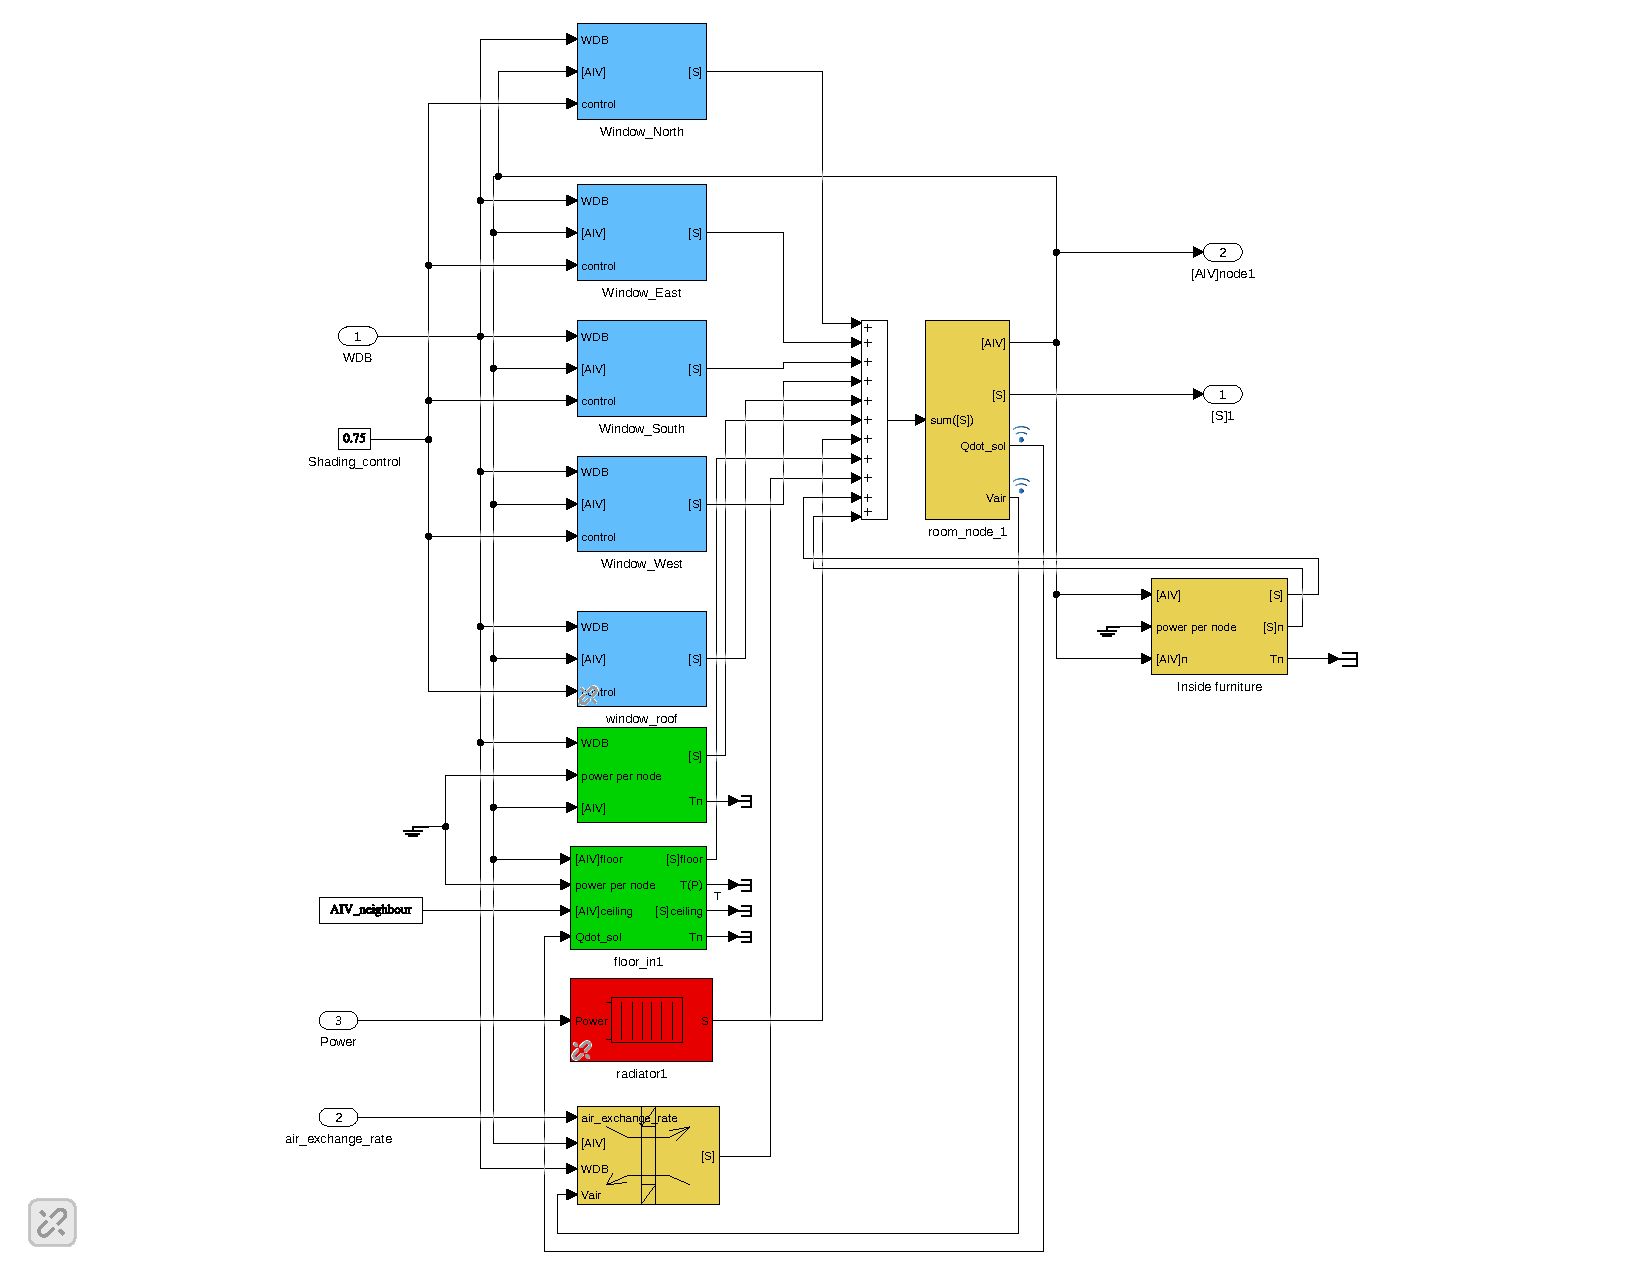
\includegraphics[width = \textwidth]{Images/polydome_room_model.pdf}
    \caption{Simulink Schema of the CARNOT \pdome\ building model}
    \label{fig:CARNOT_polydome}
\end{figure}

\clearpage

The Simulink model is then completed by adding a \textit{Weather Data File}
containing weather measurements for a whole year, and a \textit{Weather
Prediction} block responsible for sending weather predictions to the MPC.\@ The
controller itself is defined in Python and is connected to Simulink via three
TCP/IP sockets: one for sending the control signal, one for reading the
temperature measurement, and one for reading the weather forecast.

The final Simulink schema is presented in Figure~\ref{fig:CARNOT_complete}:

\begin{figure}[ht]
    \centering
    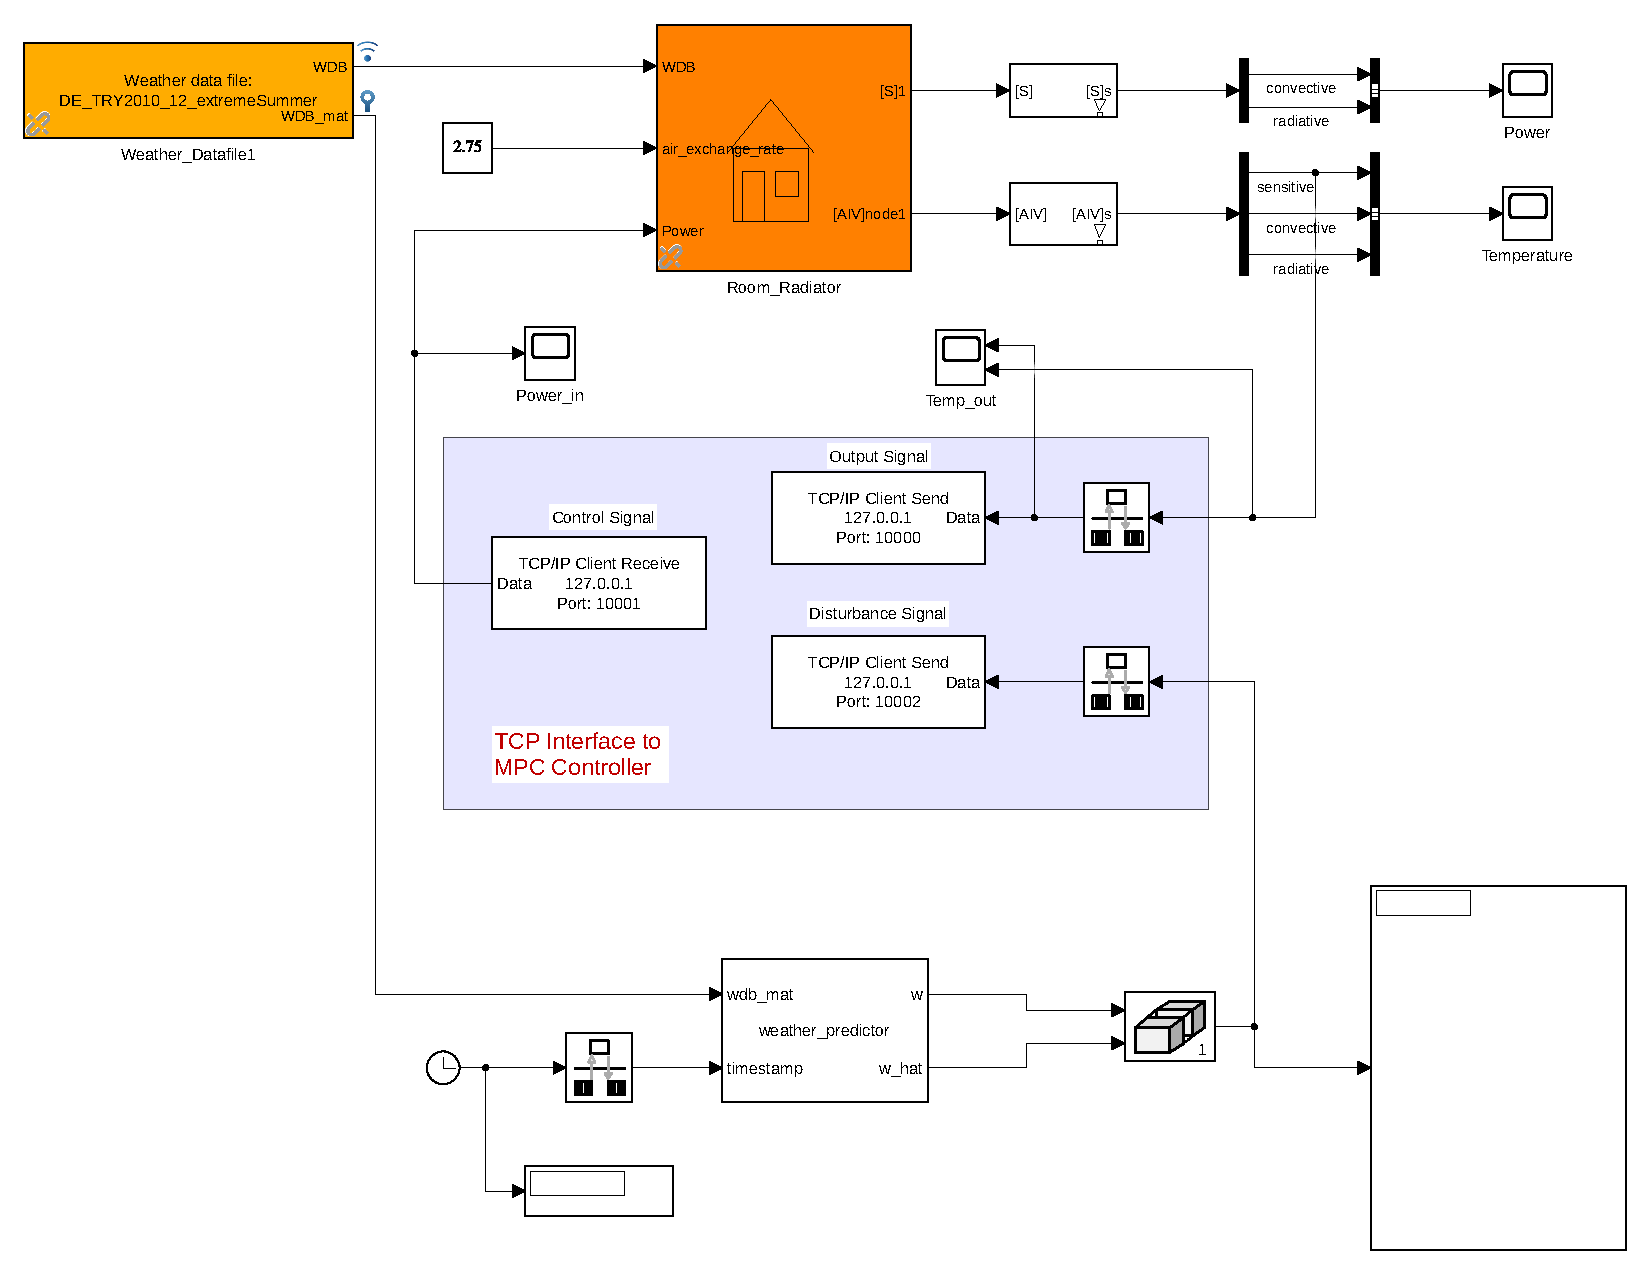
\includegraphics[width = \textwidth]{Images/polydome_python.pdf}
    \caption{Simulink Schema of the Complete Simulation}
    \label{fig:CARNOT_complete}
\end{figure}

\clearpage

\subsection{Physical dimensions}\label{sec:Physical_dimensions}

The \pdome\ building is a dome-shaped, single-zone building serving the role
of classroom for audiences of around one hundred students.

Most of the necessary measurements are already available from the
\citetitle*{nattererPolydomeTimberShell1993} article by
\textcite{nattererPolydomeTimberShell1993}. It presents the \pdome\ geometry as
having a floor area of 25m $\times$ 25m, a maximum height of the building of 7m,
walls of a maximum height of 3m. The roof is a spherical cap with a radius of
approximately 28m.

One particularity of the \pdome\  is the presence of four large skylights on the
roof. An estimate of their size has been made using images from \textit{Google
Maps Satellite View}~\cite{GoogleMaps}, with the included measurement tool. These
measurements are presented in Figure~\ref{fig:Google_Maps_Skylights}. The
skylights are measured to be squares of edge 2.5m.

\begin{figure}[ht]
    \centering
    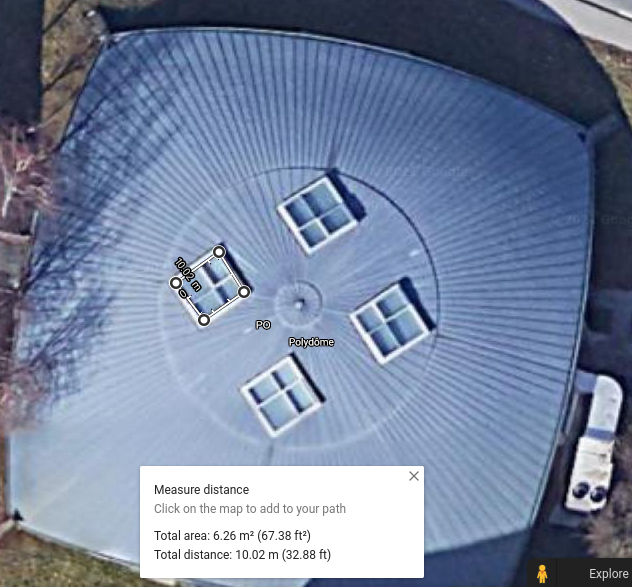
\includegraphics[width = 0.8\textwidth]{Images/google_maps_polydome_skylights}
    \caption{Google Maps Satellite view of the \pdome\ building}
    \label{fig:Google_Maps_Skylights}
\end{figure}

The only remaining missing piece of information is the \textit{stem wall}
height, which is the height of the walls from the ground on which the dome
ceiling directly resides. Due to the limited campus access, this measure has
also been approximated from a Google Maps image, presented in
Figure~\ref{fig:Google_Maps_Streetview}. An object of known size has been used
as reference, after which the following measurements have been done in
\citetitle{kimballGIMPGNUImage}~\cite{kimballGIMPGNUImage} using the
\textit{Measure Tool}.

The chosen reference object is the \pdome\ HVAC system, the full description of
which is presented in Section~\ref{sec:HVAC_parameters}, and which has a known
height of 2061mm \cite{aermecRoofTopManuelSelection}.

\begin{figure}[ht]
    \centering
    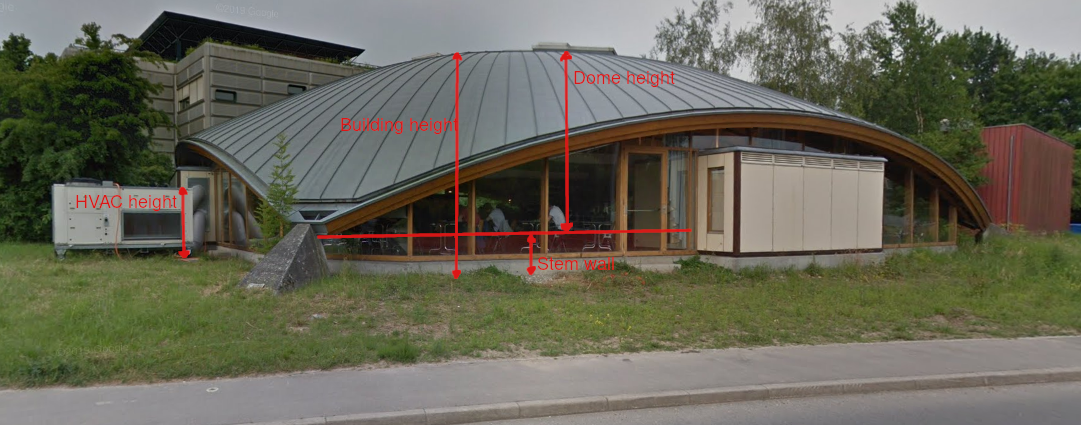
\includegraphics[width = \textwidth]{Images/polydome_streetview_annotated}
    \caption{Google Maps StreetView view of the \pdome\ building}
    \label{fig:Google_Maps_Streetview}
\end{figure}

The graphical analysis resulted in the measurements presented in
Table~\ref{tab:GIMP_measurements}:

\begin{table}[ht]
%\vspace{-8pt}
\centering
    \begin{tabular}{||c c c c||}
        \hline
        Object & Size [px] & Size[mm] & Size[m]\\
        \hline \hline
        HVAC height & 70 & 2100 & 2.1 \\
        Building height & 230 & 6900 & 6.9 \\
        Stem wall & 45 & 1350 & 1.35 \\
        Dome height & 185 & 5550 & 5.55 \\
        \hline
    \end{tabular}
\caption{Calculated Dome Dimensions}
\label{tab:GIMP_measurements}
\end{table}

For a validation of the results shown in Figure~\ref{tab:GIMP_measurements} it
is possible to compare the total \pdome\ building height measured in GIMP with
the value presented beforehand. The graphical measure of 6.9m is indeed very
close to the described height of 7m.

These measurements can be used to set the size parameters of all the nodes in
the model:

\begin{itemize}
    \item Side windows with a size of 2m $\times$ 25m each
    \item Roof window with a size of 5m $\times$ 5m, cumulative surface of all
        the skylights
    \item Ceiling with a size of 25m $\times$ 25m
    \item Floor with a size of 25m $\times$ 25m
\end{itemize}

\subsection{Internal volume}

The \pdome\ building has a structure that is mostly based on a dome shape, with
the difference that the dome portion of the building does not reach the ground,
but stands above it at a height of $\approx 1.35m$ (cf.
Table~\ref{tab:GIMP_measurements}), with the large side windows extending to the
ground and creating a \textit{stem wall} for the dome to sit on.

The total internal volume of the \pdome\ building can therefore be approximated
by computing the sum volumes of the two elements: the stem and the dome.

Geometrically, a dome is a portion of a sphere cut off by a plane. Its volume
can therefore be computed in a similar fashion to that of a complete sphere.

A sphere can be regarded as volume of rotation of function $f(x)$ (cf.
Equation~\ref{eq:rot_func}) around the x axis, where $R$ is the sphere radius
and $x \in [0, 2r]$: 

\begin{equation}\label{eq:rot_func}
    f(x) = \sqrt{R^2 - (x-R)^2} = \sqrt{2Rx - x^2}
\end{equation}

It is therefore possible to compute the volume of a dome by integrating $f(x)$
up to the dome height $h$, as presented in Equation~\ref{eq:rot_vol}. 

\begin{equation}\label{eq:rot_vol}
    \begin{aligned}
        V &= \pi \int_0^h f(x)^2 dx \\
          &= \pi \int_0^h (2Rx - x^2)dx \\
          &= \pi \left( Rx^2 - \frac{1}{3}x^3 \right)_0^h \\
          &= \frac{\pi h^2}{3} (3R - h) \\
    \end{aligned}
\end{equation}

The volume of the \pdome\ dome is computed  by first finding the radius of the
complete sphere, the radius of curvature (cf.
Equation~\ref{eq:radius_curvature}, where $h$ is the height of the dome and $r$
is the radius of the base of the dome) and plugging it in
Equation~\ref{eq:rot_vol}.

\begin{equation}\label{eq:radius_curvature}
    R_c = \frac{r^2 + h^2}{2h}
\end{equation}

The volume of the dome is then given by: 

\begin{equation}
    V_d = \frac{1}{3} \pi h^2 (3R_c - h) = \frac{1}{6} \pi h (3r^2 + h^2)
\end{equation}

The stem of the \pdome\ is approximated to a cube of edge 25m, and its volume can
therefore be calculated as: 

\begin{equation}
    V_s = l_s^2 * h_s
\end{equation}

The total volume of the building is then given as: 

\begin{equation}
    V = V_d + V_s = \frac{1}{6} \pi h (3r^2 + h^2) + l_s^2
\end{equation}

Numerically, considering a dome diameter of 28m, a dome height of 5.55m and a stem
wall edge of 25m, we get the approximate volume of the building:
\begin{equation}\label{eq:numerical_volume}
    V = V_d + V_s = 1798.22m^3 + 843.75m^3 = 2641.97m^3 \approx 2650m^3
\end{equation}

The value presented in Equation~\ref{eq:numerical_volume} is used directly in
the \textit{room\_node} of the CARNOT model (cf.
Figure~\ref{fig:CARNOT_polydome}), as well as the calcualtion of the Air
Exchange Rate, presented in Section~\ref{sec:Air_Exchange_Rate}.

\subsection{Furniture}

The main function of the \pdome\ building is serving as a classroom for around
one hundred students. It has wood furniture consisting of chairs and tables, as
well as a wooden stage in the center of the building, meant to be used for
presentations. The building also contains a smaller room, housing the all the
necessary technical equipment (cf. Figure~\ref{fig:Google_Maps_Streetview}).

The most accurate way of including information on the furniture in the CARNOT
model would be to manually compute the mass, volume and materials for each of
the chairs, tables, etc.\ but due to the restricted access to the building a
simpler approximation has been made.

\textcite{johraNumericalAnalysisImpact2017} present a methodology to model the
furniture in buildings for multiple different materials, as well as an
\textit{equivalent indoor content material} that is meant to approximate the
furniture content of an office building. These values for mass content, surface
area, material density and thermal conductivity have been taken as the basis for
the \pdome\ furniture content approximation, with the assumption that, since the
\pdome\ is still mostly empty, it has approximately a quarter of the furniture
present in a fully furnished office.

The full set of furniture is therefore approximated in the CARNOT model as a
wall, with the numerical values for mass, surface, thickness and volume
presented below.

\subsubsection*{Surface}
% surface:
% 1/4 * 1.8 [m2/m2 of floor space] * 625 m2 surface = 140 m2
% 140 m2 = [7 20] m [height width]

The equivalent material is taken to have a surface of 1.8 $m^2$ per each $m^2$
of floor area~\cite{johraNumericalAnalysisImpact2017}. With a floor area of 625
$m^2$, and assuming the furnishing of the building is a quarter that of a
fully-furnished office, the \pdome\ furniture equivalent wall has a surface area
of:

\begin{equation}
    S_f = \frac{1}{4} \cdot 1.8 \left[\frac{\text{m}^2}{\text{m}^2}\right]
    \cdot 625\ \left[\text{m}^2\right] = 140\ \left[\text{m}^2\right]
\end{equation}

\subsubsection*{Mass}
% mass:
% 1/4 * 40 [kg/m2 of floor space] * 625 m2 surface = 6250 kg

The mass of the furniture equivalent wall is computed using the same
methodology, considering 40 kg of furniture mass per $m^2$ of floor surface.

\begin{equation}
    M_f = \frac{1}{4} \cdot 40 \cdot 625\ \left[\text{m}^2\right] = 6250\
    \left[\text{m}^2\right]
\end{equation}

\subsubsection*{Volume}
% volume:
% 6250[kg]/600[kg/m3] = 10.41 [m3]

The volume of the furniture equivalent wall is calculated with the help of the
equivalent mass and densities:

\begin{equation}
    V_f = \frac{M_f}{\rho_f} = \frac{6250}{600}
    \left[\frac{\text{kg}}{\text{kg}/\text{m}^3}\right]
    = 10.41\ \left[\text{m}^3\right]
\end{equation}

\subsubsection*{Thickness}
% thickness:
%10.41[m3]/140[m2] = 0.075m = 7.5cm

The last parameter of the furniture equivalent wall is computed by dividing its
volume by the surface:

\begin{equation}
    h_f = \frac{V_f}{S_f} = \frac{10.41}{140} \left[\frac{m^3}{m^2}\right] =
    0.075\ \left[\text{m}\right] = 7.5\ \left[\text{cm}\right]
\end{equation}


\subsection{Material properties}

In order to better simulate the behaviour of the real \pdome\ building it is
necessary to approximate the building materials and their properties as close as
possible. This section goes into the detailes and arguments for the choice of
parameters for each of the CARNOT nodes' properties.

\subsubsection{Windows}

The windows are supposed to be made of two glass panes of thickness 4mm each.

The values of the heat transfer coefficient (U-factor) can vary greatly for
different window technologies, but an educated guess can be made on the lower
and upper bounds based on the age and location of the building. 

Window manufacturers state
the U-factor for double glass windows to be between 2.8 \(\frac{W}{m^2K}\) for
older manufacturing techniques and 1.2 \(\frac{W}{m^2K}\) for newer
models~\cite{WhatAreTypical2018}. 

The US Energy Department states that the
typical U-factor values for modern window installations is in the range of 0.2
--- 1.2 \(\frac{W}{m^2K}\)\cite{GuideEnergyEfficientWindows}. 

The European flat glass association claims that the maximum allowable U-factor
value for new window installations in the private sector buildings in
Switzerland is 1.5
\(\frac{W}{m^2K}\)~\cite{glassforeuropeMinimumPerformanceRequirements2018}.

Considering the aforementioned values, and the fact the the \pdome\ building was
built in 1993~\cite{nattererModelingMultilayerBeam2008}, the default U-factor of
1.8 \(\frac{W}{m^2K}\) has been deemed appropriate.

The total solar energy transmittance $[g]$ and transmittance in the visible
range $[v_g]$ can vary in the range of 0.1 --- 0.9 depending on manufacturing
technology, tint, etc. The average values of 0.7 and 0.65 respectively have been
chosen for this case.

The values for glass density and heat capacity have been left at their default
values of 2500 \(\frac{kg}{m^3}\) and 1008 \(\frac{J}{kgK}\) respectively.

\subsubsection{Roof and Floor}

%%% Roof
% [5cm wood, 10cm insulation, 5cm wood]
% Conductivity for each material
% Heat capacity for each material
% Density for each material

The roof structure has been assumed to be made out of 10cm of insulation,
enclosed on each side by 5cm of wood.

%%% Floor
% [5cm wood, 10cm insulation, 20cm concrete]
% Conductivity for each material
% Heat capacity for each material
% Density for each material

The floor composition has been taken as consisting of, from top to bottom, 5cm
wood, 10cm insulation followed by 20cm of concrete. 

All the necessary values to characterise these materials have been taken
from~\cite{BuildingsHeatTransferData} and are presented in
Table~\ref{tab:material_properties}: 

\begin{table}[ht]
%\vspace{-8pt}
\centering
    \begin{tabular}{||c c c c||}
        \hline
        Material & Thermal Conductivity $[k]$ $[\frac{W}{mK}]$ & Specific Heat
        Capacity $[c]$ $[\frac{J}{kgK}]$ & Density $[\rho]$ $[\frac{kg}{m^3}]$
        \\
        \hline \hline
        Plywood & 0.12 & 1210 & 540 \\
        Insulation & 0.03 & 1200 & 40 \\
        Concrete & 1.0 & 700 & 2500 \\
        \hline
    \end{tabular}
    \caption{Material properties for roof and floor elements}
\label{tab:material_properties}
\end{table}

\subsection{HVAC parameters}\label{sec:HVAC_parameters}

The \pdome\ is equiped with an \textit{AERMEC RTY-04} HVAC system. According to
the manufacturer's manual~\cite{aermecRoofTopManuelSelection}, this HVAC houses
two compressors, of power 11.2 kW and 8.4 kW respectively, an external
ventillator of power 1.67 kW, and a reflow ventillator of power 2 kW. The unit
has a typical Energy Efficiency Ratio (EER, cooling efficiency) of 4.9 --- 5.1
and a Coefficient of Performance (COP, heating efficiency) of 5.0, for a maximum
cooling capacity of 64.2 kW. 

One particularity of this HVAC unit is that during summer only one of the two
compressors are running. This results in a higher EER, in the cases where the
full cooling capacity is not required.

\subsubsection*{Ventilation}

According to the manufacturer manual \cite{aermecRoofTopManuelSelection}, the
HVAC unit's external fan has an air debit ranging between 4900
$\text{m}^3/\text{h}$ and 7000 $\text{m}^3/\text{h}$.

\subsubsection*{Air Exchange Rate}\label{sec:Air_Exchange_Rate}

The air exchange rate, also known as `air changes per hour', represents the
number of times the air in a room gets replaced with new air. It can be
computed by dividing the air flow through the room by the room volume:

\begin{equation}
    \text{Air exchange rate} = \frac{\text{Air flow}}{\text{Total volume}}
\end{equation}

In the case of the \pdome\ and its HVAC, this results in an airflow range of:

\begin{equation}
    \begin{aligned}
        \text{Air exchange rate} &= \frac{4900}{2650} 
        - \frac{7000}{2650} &\left[\frac{\text{m}^3/\text{h}}{\text{m}^3}\right]\\
                            &= 1.85 - 2.64 &\left[\frac{1}{\text{h}}\right]
    \end{aligned}
\end{equation}

As it will be shown in Section~\ref{sec:CARNOT_experimental}, the external fan
is continuously running. The \textit{Air exchange rate} has therefore been fixed
to a value of 2.5 for the duration of the whole simulation. The real airflow
could, of course, vary depending on a multitude of external factors, but they
would require more precise measurements to estimate.

\subsection{Validating against experimental data}\label{sec:CARNOT_experimental}

In order to confirm the validity of the model it is necessary to compare the
CARNOT models' behaviour against that of the real \pdome\ building.

Section~\ref{sec:CARNOT_expdata} presents the available experimental data,
Section~\ref{sec:CARNOT_WDB} details the transformation of the available data
into CARNOT's WDB format, and Section~\ref{sec:CARNOT_comparison} details a
qualitative analysis of the differences.

\subsubsection{The available experimental data}\label{sec:CARNOT_expdata}

All the experimental data used for the validation of the CARNOT model has been
collected previously for another
study~\cite{fabiettiMultitimeScaleCoordination2018}, where it has been used to
identify a State Space model for the \pdome\ building.

The data has been collected in the time span of June to August 2017, and is
divided in seven different experiments, as presented in
Figure~\ref{tab:exp_dates}. The available measurements are the \textit{Outside
Temperature}, \textit{Solar Irradiation}, \textit{Electrical power consumption}
of the HVAC, and two measurements of \textit{Inside Temperature} in different
parts of the room.

\begin{table}[ht]
\centering
    \begin{tabular}{||c c c||}
        \hline
        Exp no. & Start Date & End Date\\
        \hline \hline
        1 & 01.06.2017 20:00 & 03.06.2017 17:00 \\
        2 & 10.06.2017 16:00 & 12.06.2017 06:00 \\
        3 & 16.06.2017 20:00 & 19.06.2017 06:00 \\
        4 & 19.06.2017 20:00 & 22.06.2017 06:00 \\
        5 & 30.06.2017 20:00 & 03.07.2017 06:00 \\
        6 & 07.07.2017 20:00 & 10.06.2017 06:00 \\
        7 & 13.06.2017 20:00 & 20.06.2017 06:00 \\
        \hline
    \end{tabular}
\caption{\pdome\ experimental measurements}
\label{tab:exp_dates}
\end{table}

\clearpage

As mentioned previously, the external fan of the HVAC is constantly running.
This can be seen in Figure~\ref{fig:Polydome_electricity} as the electricity
consumption of the HVAC has a baseline of 1.67 kW of power consumption.

\begin{figure}[ht]
    \centering
    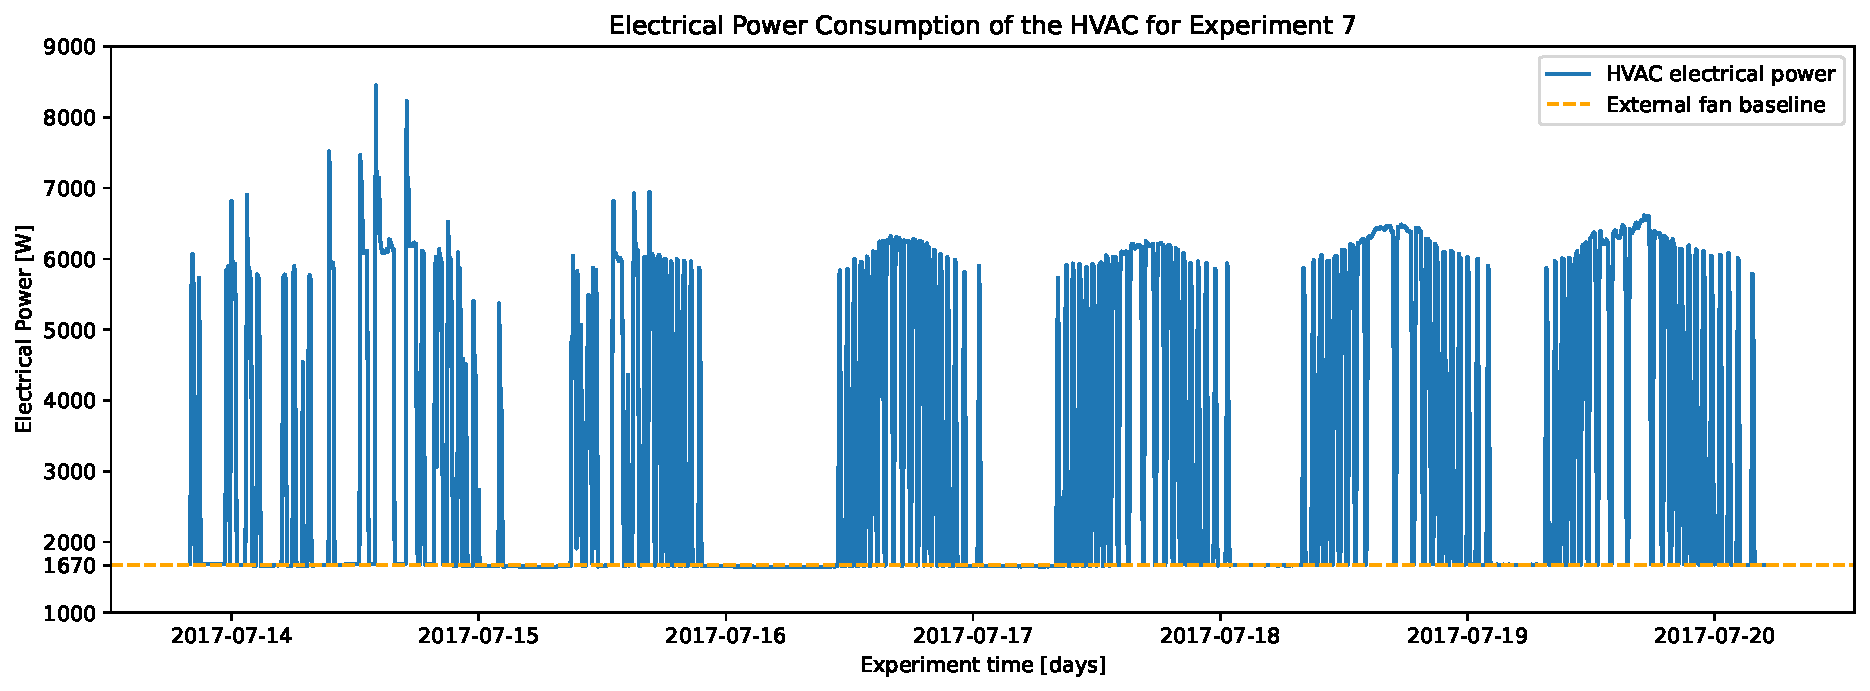
\includegraphics[width = \textwidth]{Plots/Fan_baseline.pdf}
    \caption{Electrical Power consumption of the \pdome\ HVAC for Experiment 7}
    \label{fig:Polydome_electricity}
\end{figure}

Figure~\ref{fig:Polydome_electricity} also gives an insight into the workings of
the HVAC when it comes to the combination of the two available compressors. The
instruction manual of the HVAC~\cite{aermecRoofTopManuelSelection} notes that in
summer only one of the compressors is running. This allows for a larger EER
value and thus better performance. We can see that this is the case for most of
the experiment, where the pwoer consumption caps at around 6 kW. There are,
however, moments during the first part of the experiment where the power
momentarily peaks over the 6 kW limit, and goes as high as around 9 kW. This
most probably happens when the HVAC decides that the difference between the
setpoint temperature and the actual measured values is too large.

Figure~\ref{fig:Polydome_exp7_settemp} presents the values of the setpoint
temperature and the measured internal temperature. 

\begin{figure}[ht]
    \centering
    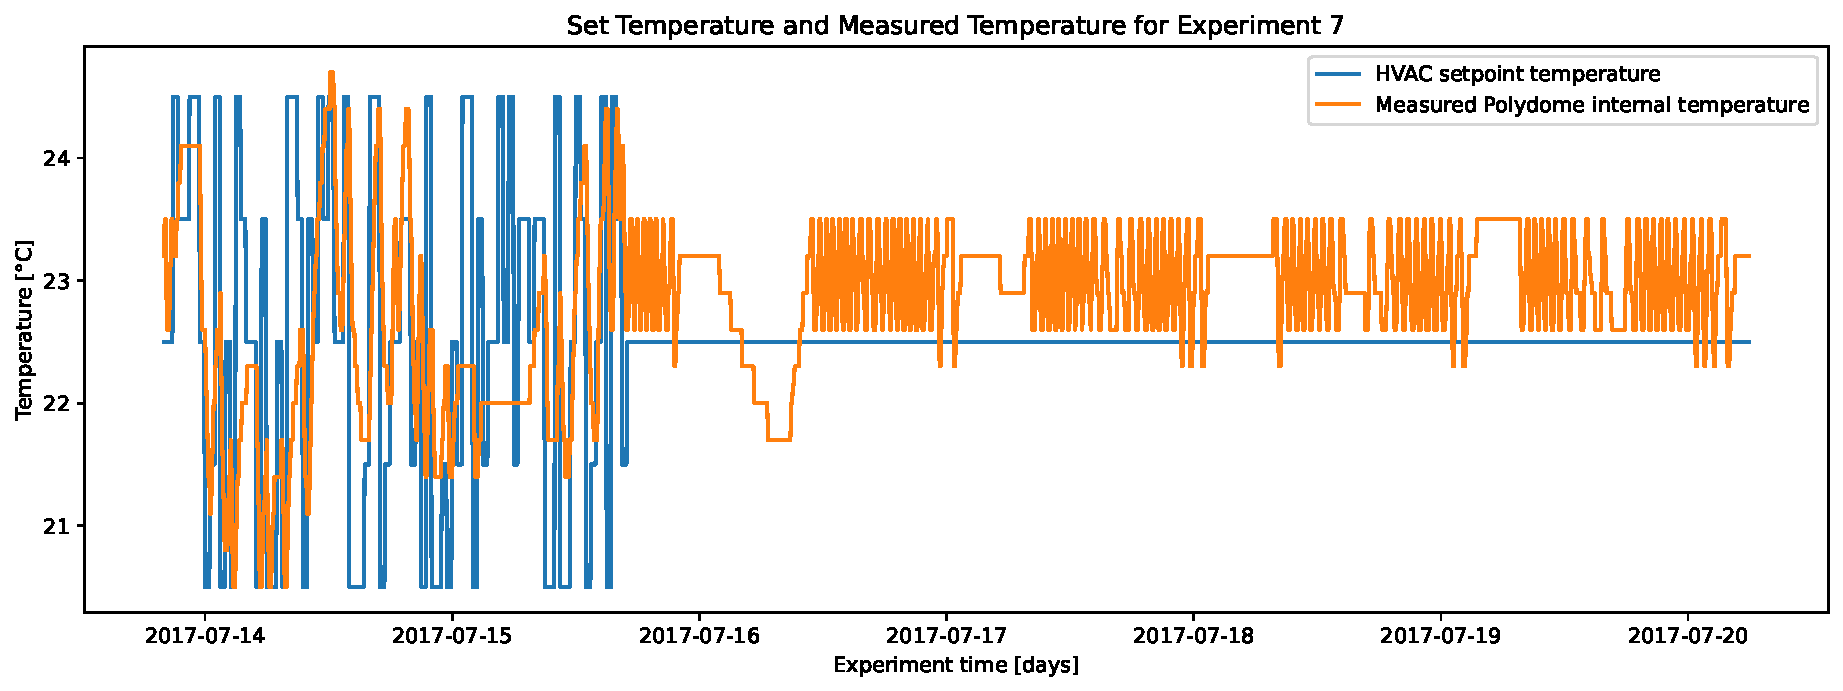
\includegraphics[width = \textwidth]{Plots/Exp_settemp.pdf}
    \caption{Measured vs setpoint temperature of the HVAC for Experiment 7}
    \label{fig:Polydome_exp7_settemp}
\end{figure}

A few observations can be made on these measurements. First, the second
compressor is indeed turned on during the first part of the experiment, when the
setpoint differs greatly from the measured temperature. Second, for the
beginning of Experiment 7, as well as the majority of the other experiments, the
setpoint temperature is the value that gets changed in order to excite the
system, and since the HVAC's controller is on during identification, it will
oscillate between using one or two compressors. Lastly, it is possible to notice
that the HVAC is not turned on during the night, with the exception of the
external fan, which runs continuously.

\subsubsection{The CARNOT WDB weather data format}\label{sec:CARNOT_WDB}

For a corect simulation of the building behaviour, CARNOT requires not only the
detailed definition of the building blocks/nodes, but also a very detailed set
of data on the weather conditions. This set includes detailed information on the
sun's position throughout the simulation (zenith and azimuth angles), the Direct
Normal Irradiance (DHI) and Direct Horizontal Irradiance (DNI), direct and
diffuse solar radiation on surface, as well as information on the ambient
temperature, humidity, precipitation, pressure, wind speed and direction, etc.
A detailed overview of each measurement necessary for a simulation is given in
the CARNOT user manual~\cite{CARNOTManual}.

In order to compare the CARNOT model's performance to that of the real \pdome\
it is necessary to simulate the CARNOT model under the same set of conditions as
the ones present during the experimental data collection. In order to do this,
all the missing values that are required by the simulation have to be filled. In
some cases, such as the sun angles it is possible to compute the exact values,
but in other cases the real data is not available, which means that is has to be
inferred from the available data.

The information on the zenith and azimuth solar angles can be computed exactly
if the position and elevation of the building are known. The GPS coordinates and
elevation information is found using a map~\cite{ElevationFinder}. With that
information available, the zenith, azimuth angles, as well as the angle of
incidence (AOI) are computed using the Python pvlib
library~\cite{f.holmgrenPvlibPythonPython2018}.

As opposed to the solar angles which can be computed exactly from the available
information, the Solar Radiation Components (DHI and DNI) have to be estimated
from the available measurements of GHI, zenith angles (Z) and datetime
information.  \textcite{erbsEstimationDiffuseRadiation1982} present an empirical
relationship between GHI and the diffuse fraction DF and the ratio of GHI to
extraterrestrial irradiance $K_t$, known as the Erbs model. The DF is then used
to compute DHI and DNI as follows:

\begin{equation}
    \begin{aligned}
        \text{DHI} &= \text{DF} \times \text{GHI} \\
        \text{DNI} &= \frac{\text{GHI} - \text{DHI}}{\cos{\text{Z}}}
    \end{aligned}
\end{equation}

All the other parameters related to solar irradiance, such as the in-plane
irradiance components, in-plane diffuse irradiances from the sky and the ground
are computed using the Python pvlib.

The values that cannot be either calculated or approximated from the available
data, such as the precipitation, wind direction, incidence angles in place of
vertical and main/secondary surface axis have been replaced with the default
CARNOT placeholder value of -9999. The relative humidity, cloud index, pressure
and wind speed have been fixed to 50\%, 0.5, 96300 Pa, 0 $\text{m}/\text{s}$
respectively.

\subsubsection{\pdome\ and CARNOT model comparison}\label{sec:CARNOT_comparison}

With the WDB data compiled, we can now turn to simulating the CARNOT model and
compare its behaviour to that of the real \pdome\ building. 

Unfortunately, one crucial piece of information is missing: the amount of heat
the HVAC either pumps in or takes out of the building at any point in time. This
value could be approximated from the information of electrical power consumption
and the EER, COP values given that it is known if the HVAC is in either heating
or cooling mode. 

This information lacking in the existing experimental datasets, the heat
supplied/ taken out of the system has been inferred from the electrical energy
use, measured building temperature and HVAC temperature setpoint, with the
assumption that the HVAC is in cooling mode whenever the measurements are
higher than the setpoint temperature, and is in heating mode otherwise. As it
can already be seen in Figure~\ref{fig:Polydome_exp7_settemp}, this is a very
strong assumption, that is not necessarily always correct. It works well when
the measurements are very different from the sepoint, as is the case in the
first part of the experiment, but this assumption is false for the second part
of the experiment, where the sepoint temperature remains fixed and it is purely
the HVAC's job to regulate the temperature.

\begin{figure}[ht]
    \centering
    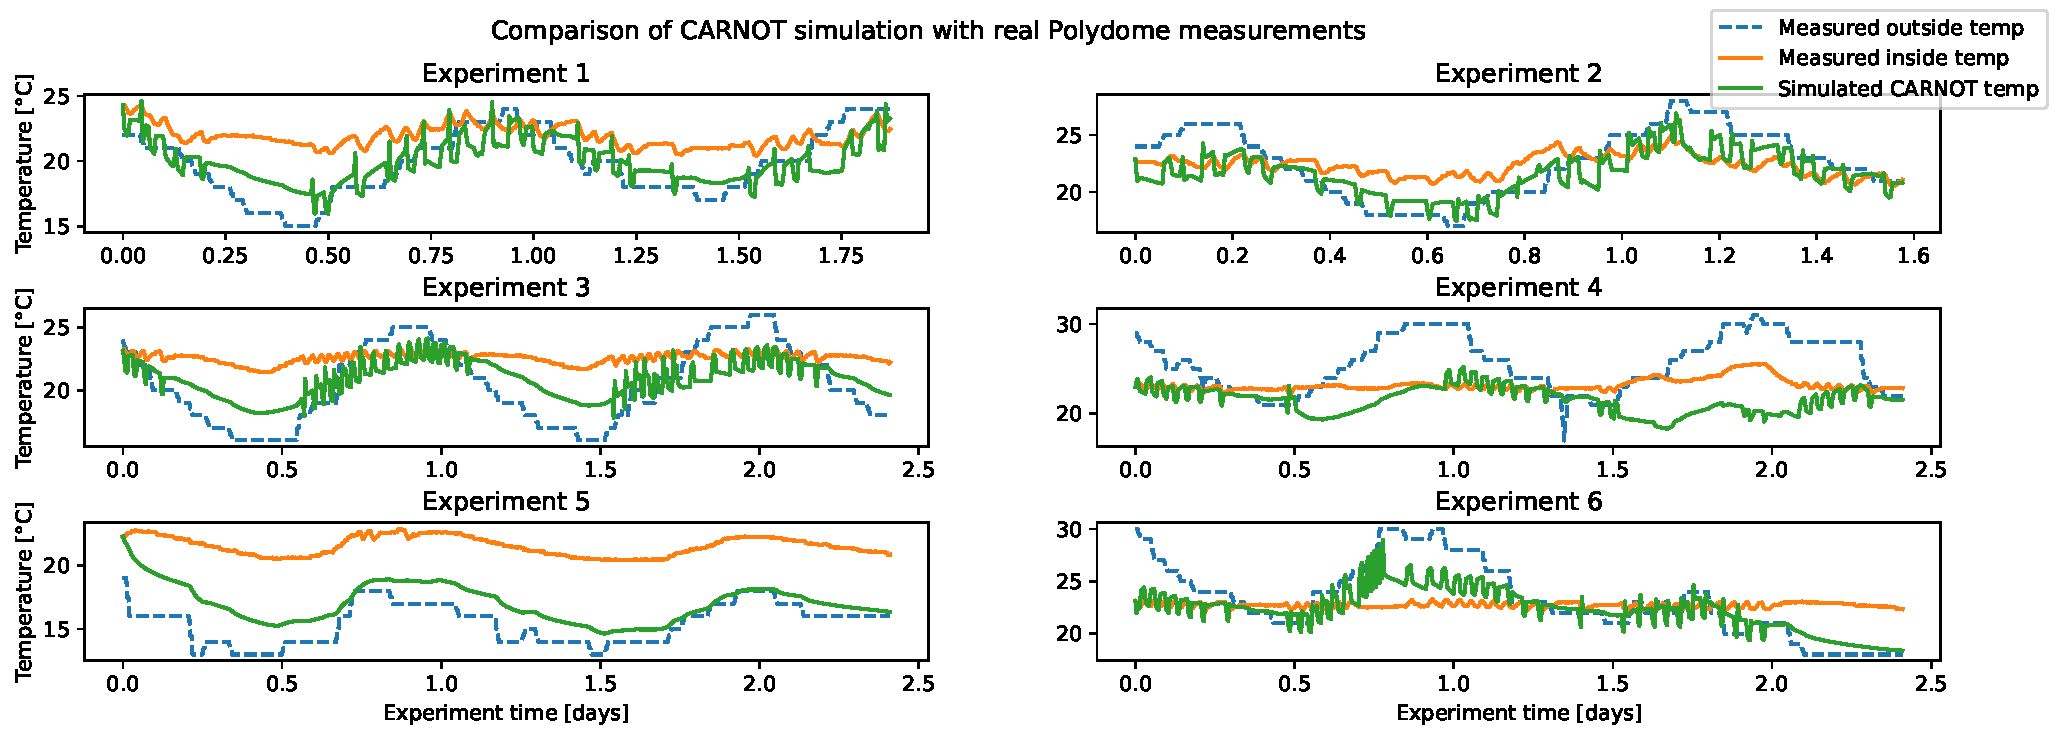
\includegraphics[width = \textwidth]{Plots/CARNOT_comparison_1.pdf}
    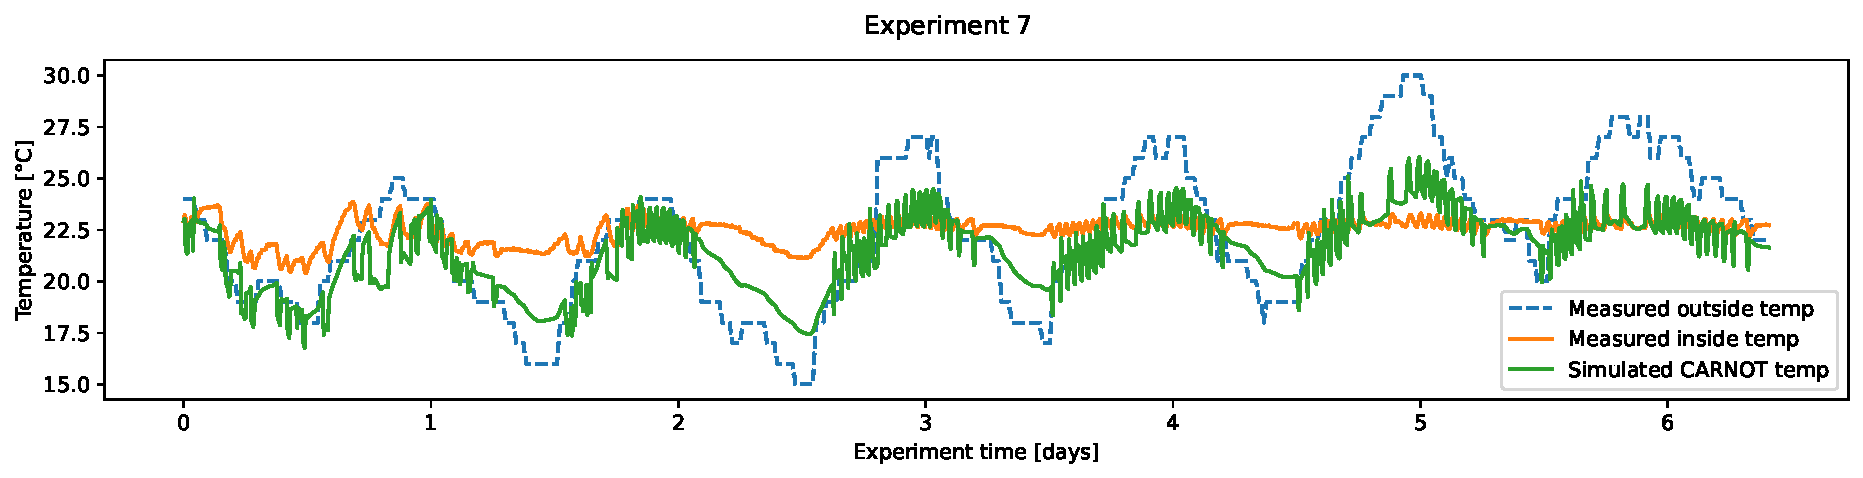
\includegraphics[width = \textwidth]{Plots/CARNOT_comparison_2.pdf}
    \caption{Measured vs CARNOT simulated temperature for the Experimental
    Datasets}
    \label{fig:CARNOT_simulation_validation}
\end{figure}

The results of the seven simulations are presented in
Figure~\ref{fig:CARNOT_simulation_validation}. Overall, the simulated
temperature has the same behaviour as the real \pdome\ measurements. A more
detailed inspection shows that for most of the experiments the simulated
temperature is much more volatile than the true measurements. This could be due
to an overestimated value of the Air Exchange Rate, underestimated amount of
furniture in the building, or, more probably, miscalculation of the HVAC's
heating/cooling mode. Of note is the large difference in behaviour for the
Experiments 5 and 6. In fact, for these experiments, the values for the
electical power consumption greatly differ in shape from the ones presented in
the other datasets, which could potentially mean erroneous measurements, or some
other underlying problem with the data.

Finally, it is possible to conclude that the CARNOT building behaves comparably
to the real \pdome\, even if not perfectly simulates its behaviour. These
differences  could come from multiple factors, missing information that had to
be inferred and/or approximated, such as the Air Exchange Ratio, the heat
provided/extracted, the amount of furniture in the building, the overall shape
and size of the building, as well as possibly errors in the experimental data
used for validation. A more detailed analysis of the building parameters would
have to be done in order to find the reason and eliminate these discrepancies.


\clearpage

\section{Choice of Hyperparameters}

This section will discuss and try to validate the choice of all the
hyperparameters necessary for the training of a \acrshort{gp} model to capture
the CARNOT building's behaviour.

The class of black-box models is very versatile, being able to capture plant
behaviour directly from data. This comes in contrast to white-box and grey-box
modelling techniques, which require much more physical insight into the plant's
behaviour.

The advantage of black-box models lies in the lack of physical parameters to be
fitted. On the flip side, this versatility of being able to fit much more
complex models purely on data comes at the cost of having to properly define the
model hyperparameters: the number of regressors, the number of autoregressive
lags for each class of inputs, the shape of the covariance function have to be
taken into account when designing a \acrshort{gp} model. These choices have
direct influence on the resulting model behaviour and where it can be
generalized, as well as indirect influence in the form of more expensive
computations in the case of larger number of regressors and more complex kernel
functions.

As described in Section~\ref{sec:gp_dynamical_system}, for the purpose of this
project the \acrlong{gp} model will be trained using the \acrshort{narx}
structure. This already presents an important choice in the selection of
regressors and their respective autoregressive lags.

The output of the model has been chosen as the \textit{temperature measured
inside} the CARNOT building. This is a suitable choice for the \acrshort{ocp}
defined in Section~\ref{sec:mpc_problem}, where the goal is tracking as close as
possible the inside temperature of the building.

The input of the \acrshort{gp} model coincides with the input of the CARNOT
building, namely the \textit{power} passed to the idealized \acrshort{hvac},
which is held constant during the complete duration of a step.

As for the exogenous inputs the choice turned out to be more complex. The CARNOT
WDB format (cf. Section~\ref{sec:CARNOT_WDB}) consists of information of all the
solar angles, the different components of solar radiation, wind speed and
direction, temperature, precipitation, etc. All of this information is required
in order for CARNOT's proper functioning. 

Including all of this information into the \acrshort{gp}s exogenous inputs would
come with a few downsides. First, depending on the number of lags chosen for the
exogenous inputs, the number of inputs to the \acrshort{gp} could be very large,
an exogenous inputs vector of 10 elements with 2 lags would yield 20 inputs for
the \acrshort{gp} model. This is very computationally expensive both for
training and using the model, as its algorithmic complexity is
$\mathcal{O}(n^3)$.

Second, this information may not always available in experimental
implementations on real buildings, where legacy equipment might already be
installed, or where budget restrictions call for simpler equipment.  An example
of this are the experimental datasets used for validation of the CARNOT model,
where the only available weather information is the \acrshort{ghi} and the
measurement of the outside temperature. This would also be a limitation when
getting the weather predictions for the next steps during real-world
experiments.

Last, while very verbose information such as the solar angles and the components
of the solar radiation is very useful for CARNOT, which simulated each node
individually, knowing their absolute positions, this information would not
always benefit the \acrshort{gp} model, at least not comparably to the
additional computational complexity.

For the exogenous inputs the choice has therefore been made to take the
\textit{Global Solar Irradiance} and \textit{Outside Temperature Measurement}.

\subsection{The Kernel}

The covariance matrix is an important choice when creating the \acrshort{gp}. A
properly chosen kernel can impose a prior desired behaviour on the
\acrshort{gp} such as continuity of the function an its derivatives,
periodicity, linearity, etc. On the flip side, choosing the wrong kernel can
make computations more expensive, require more data to learn the proper
behaviour or outright be numerically unstable and/or give erroneous predictions.

The \acrlong{se} kernel (cf. Section~\ref{sec:Kernels}) is very versatile,
theoretically being able to fit any continuous function given enough data. When
including the \acrshort{ard} behaviour, it also gives an insight into the
relative importance of each regressor, though their respective lengthscales.

Many different kernels have been used when identifying models for building
thermal control, such as a pure Rational Quadratic
Kernel~\cite{pleweSupervisoryModelPredictive2020}, a combination of
\acrshort{se}, \acrshort{rq} and a Linear
Kernel~\cite{jainLearningControlUsing2018}, Squared Exponential Kernel and
Kernels from the M\`atern family~\cite{massagrayThermalBuildingModelling2016}.

For the purpose of this project the choice has been made to use the
\textit{\acrlong{se} Kernel}, as it provides a very good balance of versatility
and computational complexity for the modelling of the CARNOT building.

\subsection{Lengthscales}\label{sec:lengthscales}

The hyperparameters of the \acrshort{se} can be useful when studying the
importance of regressors. The larger the distance between the two inputs, the
less correlated they are. In fact, setting the kernel variance $\sigma^2$ = 1,
we can compute the correlation of two inputs located at distance one, two and
three lengthscales apart. 

\begin{table}[ht]
\centering
    \begin{tabular}{||c c ||}
        \hline
        $\norm{\mathbf{x} - \mathbf{x}'}$ &
        $\exp{(-\frac{1}{2}*\frac{\norm{\mathbf{x} - \mathbf{x}'}^2}{l^2})}$ \\
        \hline \hline
        $1l$ & 0.606 \\
        $2l$ & 0.135 \\
        $3l$ & 0.011 \\
        \hline
    \end{tabular}
\caption{Correlation of inputs relative to their distance}
\label{tab:se_correlation}
\end{table}

From Table~\ref{tab:se_correlation} is can be seen that at 3 lengthscales apart,
the inputs are already almost uncorrelated. In order to better visualize this
difference the value of relative lengthscale importance is introduced:

\begin{equation}
    \lambda = \frac{1}{\sqrt{l}}
\end{equation}

Another indicator of model behaviour is the variance of the identified
\acrshort{se} kernel. The expected value of the variance is around the variance
of the inputs. An extremely high or extremely low value of the variance could
mean a numerically unstable model.

Table~\ref{tab:GP_hyperparameters} presents the relative lengthscale importances
and the variance for different combinations of the exogenous input lags ($l_w$),
the controlled input lags ($l_u$) and the output lags ($l_y$) for a classical
\acrshort{gp} model. 

\begin{table}[ht]
%\vspace{-8pt}
\centering
    \resizebox{\columnwidth}{!}{%
    \begin{tabular}{||c c c|c|c c c c c c c c c c c||}
        \hline
        \multicolumn{3}{||c|}{Lags} & Variance &\multicolumn{11}{c||}{Kernel
        lengthscales relative importance} \\
            $l_w$ & $l_u$ & $l_y$ & $\sigma^2$ &$\lambda_{w1,1}$ & $\lambda_{w1,2}$ &
            $\lambda_{w1,3}$ & $\lambda_{w2,1}$ & $\lambda_{w2,2}$ &
            $\lambda_{w2,3}$ & $\lambda_{u1,1}$ & $\lambda_{u1,2}$ &
            $\lambda_{y1,1}$ & $\lambda_{y1,2}$ & $\lambda_{y1,3}$\\
        \hline \hline
        1 & 1 & 1 & 0.11 & 0.721 &  &  & 2.633 &  &  & 0.569 &  & 2.645 &  &  \\
        1 & 1 & 2 & 22.68 & 0.222 &  &  & 0.751 &  &  & 0.134 &  & 3.154 & 3.073
          &  \\ 1 & 1 & 3 & 0.29 & 0.294 &  &  & 1.303 &  &  & 0.356 &  & 2.352
          & 1.361 & 2.045 \\ 1 & 2 & 1 & 7.55 & 0.157 &  &  & 0.779 &  &  &
        0.180 & 0.188 & 0.538 &  &  \\ 1 & 2 & 3 & 22925.40 & 0.018 &  &  &
        0.053 &  &  & 0.080 & 0.393 & 0.665 & 0.668 & 0.018 \\ 2 & 1 & 2 & 31.53
              & 0.010 & 0.219 &  & 0.070 & 0.719 &  & 0.123 &  & 3.125 & 3.044 &
              \\ 2 & 1 & 3 & 0.44 & 0.007 & 0.251 &  & 0.279 & 1.229 &  & 0.319
                   &  & 2.705 & 1.120 & 2.510 \\ 3 & 1 & 3 & 0.56 & 0.046 &
              0.064 & 0.243 & 0.288 & 1.151 & 0.233 & 0.302 &  & 2.809 & 1.086 &
              2.689 \\ 3 & 2 & 2 & 1.65 & 0.512 & 0.074 & 0.201 & 0.161 & 1.225
                         & 0.141 & 0.231 & 0.331 & 0.684 & 0.064 &  \\
        \hline
    \end{tabular}%
    }
\caption{GP hyperparameter values for different autoregressive lags}
\label{tab:GP_hyperparameters}
\end{table}

In general, the results of Table~\ref{tab:GP_hyperparameters} show that the
past outputs are important when predicting future values. Of importance is also
the past inputs, with the exception of the models with very high variance, where
the relative importances stay almost constant across all the inputs. For the
exogenous inputs, the outside temperature ($w2$) is generally more important
than the solar irradiation ($w1$). In the case of more autoregressive lags for
the exogenous inputs, the more recent information is usually more important,
with a few exceptions {\color{red} Continue this sentence after considering the
2/1/3 classical GP model}

% TODO: [Hyperparameters] Classical GP parameters choice


As for the case of the \acrlong{svgp}, the results for the classical
\acrshort{gp} (cf. Table~\ref{tab:GP_hyperparameters}) are not necessarily
representative of the relationships between the regressors of the
\acrshort{svgp} model due to the fact that the dataset used for training is
composed of the \textit{inducing variables}, which are not the real data, but a
set of parameters chosen by the training algorithm in a way to best generate the
original data.

Therefore to better understand the behaviour of the \acrshort{svgp} models, the
same computations as in Table~\ref{tab:GP_hyperparameters} have been made,
presented in Table~\ref{tab:SVGP_hyperparameters}:

\begin{table}[ht]
%\vspace{-8pt}
\centering
    \resizebox{\columnwidth}{!}{%
    \begin{tabular}{||c c c|c|c c c c c c c c c c c||}
        \hline
        \multicolumn{3}{||c|}{Lags} & Variance &\multicolumn{11}{c||}{Kernel
        lengthscales relative importance} \\
            $l_w$ & $l_u$ & $l_y$ & $\sigma^2$ &$\lambda_{w1,1}$ & $\lambda_{w1,2}$ &
            $\lambda_{w1,3}$ & $\lambda_{w2,1}$ & $\lambda_{w2,2}$ &
            $\lambda_{w2,3}$ & $\lambda_{u1,1}$ & $\lambda_{u1,2}$ &
            $\lambda_{y1,1}$ & $\lambda_{y1,2}$ & $\lambda_{y1,3}$\\
        \hline \hline
                1 & 1 & 1 & 0.2970 & 0.415 &  &  & 0.748 &  &  & 0.675 &  & 0.680 &  &  \\
        1 & 1 & 2 & 0.2717 & 0.430 &  &  & 0.640 &  &  & 0.687 &  & 0.559 & 0.584 &  \\
        1 & 1 & 3 & 0.2454 & 0.455 &  &  & 0.589 &  &  & 0.671 &  & 0.522 & 0.512 & 0.529 \\
        1 & 2 & 1 & 0.2593 & 0.310 &  &  & 0.344 &  &  & 0.534 & 0.509 & 0.597 &  &  \\
        1 & 2 & 3 & 0.2139 & 0.330 &  &  & 0.368 &  &  & 0.537 & 0.447 & 0.563 & 0.410 & 0.363 \\
        2 & 1 & 2 & 0.2108 & 0.421 & 0.414 &  & 0.519 & 0.559 &  & 0.680 &  & 0.525 & 0.568 &  \\
        2 & 1 & 3 & 0.1795 & 0.456 & 0.390 &  & 0.503 & 0.519 &  & 0.666 &  & 0.508 & 0.496 & 0.516 \\
        3 & 1 & 3 & 0.1322 & 0.432 & 0.370 & 0.389 & 0.463 & 0.484 & 0.491 & 0.666 &  & 0.511 & 0.501 & 0.526 \\
        3 & 2 & 2 & 0.1228 & 0.329 & 0.317 & 0.325 & 0.334 & 0.337 & 0.331 &
        0.527 & 0.441 & 0.579 & 0.435 &  \\
        \hline
    \end{tabular}%
    }
\caption{SVGP hyperparameter values for different autoregressive lags}
\label{tab:SVGP_hyperparameters}
\end{table}

The results of Table~\ref{tab:SVGP_hyperparameters} are not very surprising, even
if very different from the classical \acrshort{gp} case. The kernel variance is
always of a reasonable value, and the relative importance of the lengthscales is
relatively constant across the board. It is certainly harder to interpret these
results as pertaining to the relevance of the chosen regressors. For the
\acrshort{svgp} model, the choice of the autoregressive lags has been made
purely on the values of the loss functions, presented in
Table~\ref{tab:SVGP_loss_functions}.

\subsection{Loss functions}

The most important metric for measuring the performance of a model is the value
of the loss function, computed on a dataset separate from the one used for
training.

There exist a number of different loss functions, each focusing on different
aspects of a model's performance. A selection of loss functions used in
identification of Gaussian Process models is presented
below~\cite{kocijanModellingControlDynamic2016}.

The \acrfull{rmse} is a very commonly used performance measure. As the name
suggests, it computes the root of the mean squared error:

\begin{equation}\label{eq:rmse}
    \text{RMSE} = \sqrt{\frac{1}{N}\sum_{i=1}^N \left(y_i -
    E(\hat{y}_i)\right)^{2}}
\end{equation}

This performance metric is very useful when training a model whose goal is
solely to minimize the difference between the values measured, and the ones
predicted by the model.

A variant of the \acrshort{mse} is the \acrfull{smse}, which normalizes the
\acrlong{mse} by the variance of the output values of the validation dataset.

\begin{equation}\label{eq:smse}
    \text{SMSE} = \frac{1}{N}\frac{\sum_{i=1}^N \left(y_i -
    E(\hat{y}_i)\right)^{2}}{\sigma_y^2}
\end{equation}

While the \acrshort{rmse} and the \acrshort{smse} are very good at ensuring the
predicted mean value of the Gaussian Process is close to the measured values of
the validation dataset, the confidence of the Gaussian Process prediction is
completely ignored. In this case two models predicting the same mean values, but
having very different confidence intervals would be equivalent according to these
performance metrics.

The \acrfull{lpd} is a performance metric which takes into account not only the
mean value of the GP prediction, but the entire distribution:

\begin{equation}
    \text{LPD} = \frac{1}{2} \ln{\left(2\pi\right)} + \frac{1}{2N}
    \sum_{i=1}^N\left(\ln{\left(\sigma_i^2\right)} + \frac{\left(y_i -
    E(\hat{y}_i)\right)^{2}}{\sigma_i^2}\right)
\end{equation}

where $\sigma_i^2$ is the model's output variance at the \textit{i}-th step.
The \acrshort{lpd} scales the error of the mean value prediction $\left(y_i -
E(\hat{y}_i)\right)^{2}$ by the variance $\sigma_i^2$. This means that the
overconfident models get penalized more than the more conservative models for
the same mean prediction error, leading to models that better represent
the real system. 

The \acrfull{msll} is obtained by subtracting the loss of the model that
predicts using a Gaussian with the mean $E(\boldsymbol{y})$ and variance
$\sigma_y^2$ of the measured data from the model \acrshort{lpd} and taking the
mean of the obtained result:

\begin{equation}
    \text{MSLL} = \frac{1}{2N}\sum_{i=1}^N\left[
        \ln{\left(\sigma_i^2\right) + \frac{\left(y_i -
        E\left(\hat{y}_i\right)\right)^2}{\sigma_i^2}}
    \right] - \frac{1}{2N}\sum_{i=1}^N\left[
        \ln{\left(\sigma_y^2\right) + \frac{\left(y_i -
        E\left(\boldsymbol{y}\right)\right)^2}{\sigma_y^2}}
    \right]
\end{equation}

The \acrshort{msll} is approximately zero for simple models and negative for
better ones.

Table~\ref{tab:GP_loss_functions} and Table~\ref{tab:SVGP_loss_functions}
present the values of the different loss functions for the same lag combinations
as the ones analyzed in Section~\ref{sec:lengthscales} for the classical
\acrshort{gp} and the \acrshort{svgp} models respectively: 

\begin{table}[ht]
%\vspace{-8pt}
\centering
    \begin{tabular}{||c c c|c c c c||}
        \hline
        \multicolumn{3}{||c|}{Lags} & \multicolumn{4}{c||}{Loss functions}\\
        $l_w$ & $l_u$ & $l_y$ & RMSE & SMSE & MSLL & LPD\\
        \hline \hline
        1 & 1 & 1 & 0.3464 & 0.36394 & 20.74 & 21.70 \\
        1 & 1 & 2 & 0.1415 & 0.06179 & -9.62 & -8.67 \\
        1 & 1 & 3 & 0.0588 & 0.01066 & -8.99 & -8.03 \\
        1 & 2 & 1 & 0.0076 & 0.00017 & 71.83 & 72.79 \\
        1 & 2 & 3 & \textbf{0.0041} & \textbf{0.00005} & 31.25 & 32.21 \\
        2 & 1 & 2 & 0.1445 & 0.06682 & -9.57 & -8.61 \\
        2 & 1 & 3 & 0.0797 & 0.02033 & -10.94 & -9.99 \\
        3 & 1 & 3 & 0.0830 & 0.02219 & \textbf{-11.48} & \textbf{-10.53} \\
        3 & 2 & 2 & 0.0079 & 0.00019 & 58.30 & 59.26 \\
        \hline
    \end{tabular}
\caption{GP Loss function values for different autoregressive lags}
\label{tab:GP_loss_functions}
\end{table}

For the classical \acrshort{gp} model (cf. Table~\ref{tab:GP_loss_functions}) a
number of different lag combinations give rise to models with very large
\acrshort{msll}/\acrshort{lpd} values. This might indicate that those models are
overconfident, either due to the very large kernel variance parameter, or the
specific lengthscales combinations. The model with the best
\acrshort{rmse}/\acrshort{smse} metrics \model{1}{2}{3} had very bad
\acrshort{msll} and \acrshort{lpd} metrics, as well as by far the largest
variance of all the combinations. On the contrary the \model{3}{1}{3} model has
the best \acrshort{msll} and \acrshort{lpd} performance, while still maintaining
small \acrshort{rmse} and \acrshort{smse} values. The inconvenience of this set
of lags is the large number of regressors, which leads to much more expensive
computations. Other good choices for the combinations of lags are
\model{2}{1}{3} and \model{1}{1}{3}, which have good performance on all four
metrics, as well as being cheaper from a computational perspective. In order to
make a more informed choice for the best hyperparameters, the performance of all
three combinations has been analysed.

\clearpage

\begin{table}[ht]
%\vspace{-8pt}
\centering
    \begin{tabular}{||c c c|c c c c||}
        \hline
        \multicolumn{3}{||c|}{Lags} & \multicolumn{4}{c||}{Loss functions}\\
        $l_w$ & $l_u$ & $l_y$ & RMSE & SMSE & MSLL & LPD\\
        \hline \hline
        1 & 1 & 1 & 0.3253 & 0.3203 & 228.0278 & 228.9843 \\
        1 & 1 & 2 & 0.2507 & 0.1903 & 175.5525 & 176.5075 \\
        1 & 1 & 3 & 0.1983 & 0.1192 & 99.7735 & 100.7268 \\
        1 & 2 & 1 & 0.0187 & 0.0012 & -9.5386 & -8.5836 \\
        1 & 2 & 3 & \textbf{0.0182} & \textbf{0.0011} & \textbf{-10.2739} &
        \textbf{-9.3206} \\
        2 & 1 & 2 & 0.2493 & 0.1884 & 165.0734 & 166.0284 \\
        2 & 1 & 3 & 0.1989 & 0.1200 & 103.6753 & 104.6287 \\
        3 & 1 & 3 & 0.2001 & 0.1214 & 104.4147 & 105.3681 \\
        3 & 2 & 2 & 0.0206 & 0.0014 & -9.9360 & -8.9826 \\
        \hline
    \end{tabular}
\caption{SVGP Loss function values for different autoregressive lags}
\label{tab:SVGP_loss_functions}
\end{table}

The results for the \acrshort{svgp} model, presented in
Table~\ref{tab:SVGP_loss_functions} are much less ambiguous. The \model{1}{2}{3}
model has the best performance according to all four metrics, with most of the
other combinations scoring much worse on the \acrshort{msll} and \acrshort{lpd}
loss functions. This has therefore been chosen as the model for the full year
simulations.


\subsection{Validation of hyperparameters}\label{sec:validation_hyperparameters}

The validation step has the purpose of testing the viability of the trained
models. If choosing a model according to loss function values on a new dataset
is a way of minimizing the possibility of over fitting the model to the training
data, validating the model by analyzing its multi-step prediction performance
ensures the model was able to learn the correct dynamics and is useful in
simulation scenarios.

The following subsections analyze the performance of the trained \acrshort{gp}
and \acrshort{svgp} models over 20-step ahead predictions. For the \acrshort{gp}
model the final choice of parameters is made according to the simulation
performance. The simulation performance of the \acrshort{svgp} model is compared
to that of the classical models while speculating on the possible reasons for
the discrepancies.

\subsubsection{Conventional Gaussian Process}

The simulation performance of the three lag combinations chosen for the
classical \acrlong{gp} models has been analysed, with the results presented in
Figures~\ref{fig:GP_113_multistep_validation},~\ref{fig:GP_213_multistep_validation}
and~\ref{fig:GP_313_multistep_validation}. For reference, the one-step ahead
predictions for the training and test datasets are presented in
Appendix~\ref{apx:hyperparams_gp}.


\begin{figure}[ht]
    \centering
    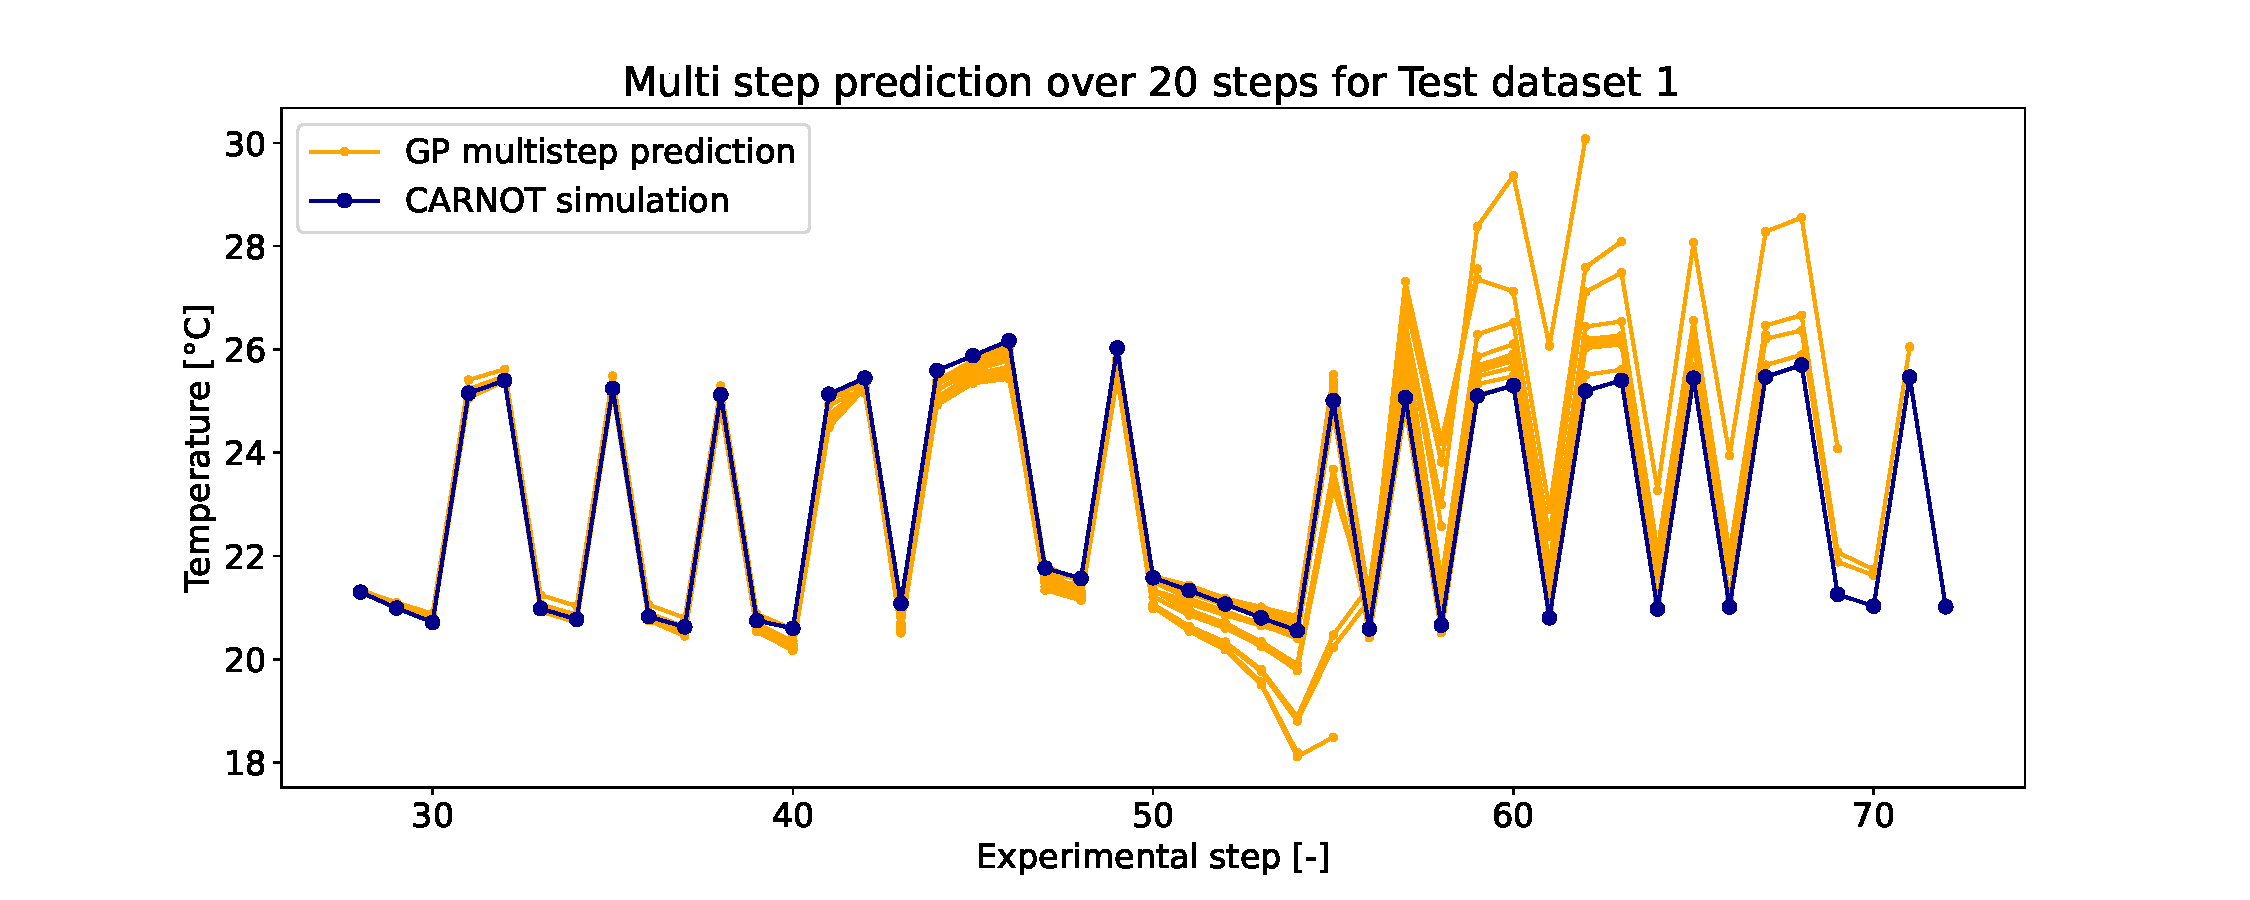
\includegraphics[width =
    \textwidth]{Plots/GP_113_-1pts_test_prediction_20_steps.pdf}
    \vspace{-25pt}
    \caption{20-step ahead simulation for \model{1}{1}{3}}
    \label{fig:GP_113_multistep_validation}
\end{figure}

In the case of the simplest model (cf.
Figure~\ref{fig:GP_113_multistep_validation}), overall the predictions are quite
good. The large deviation from true values starts happening at around 15 steps.
This could impose an additional limit on the size of the control horizon of the
\acrlong{ocp}.

\begin{figure}[ht]
    \centering
    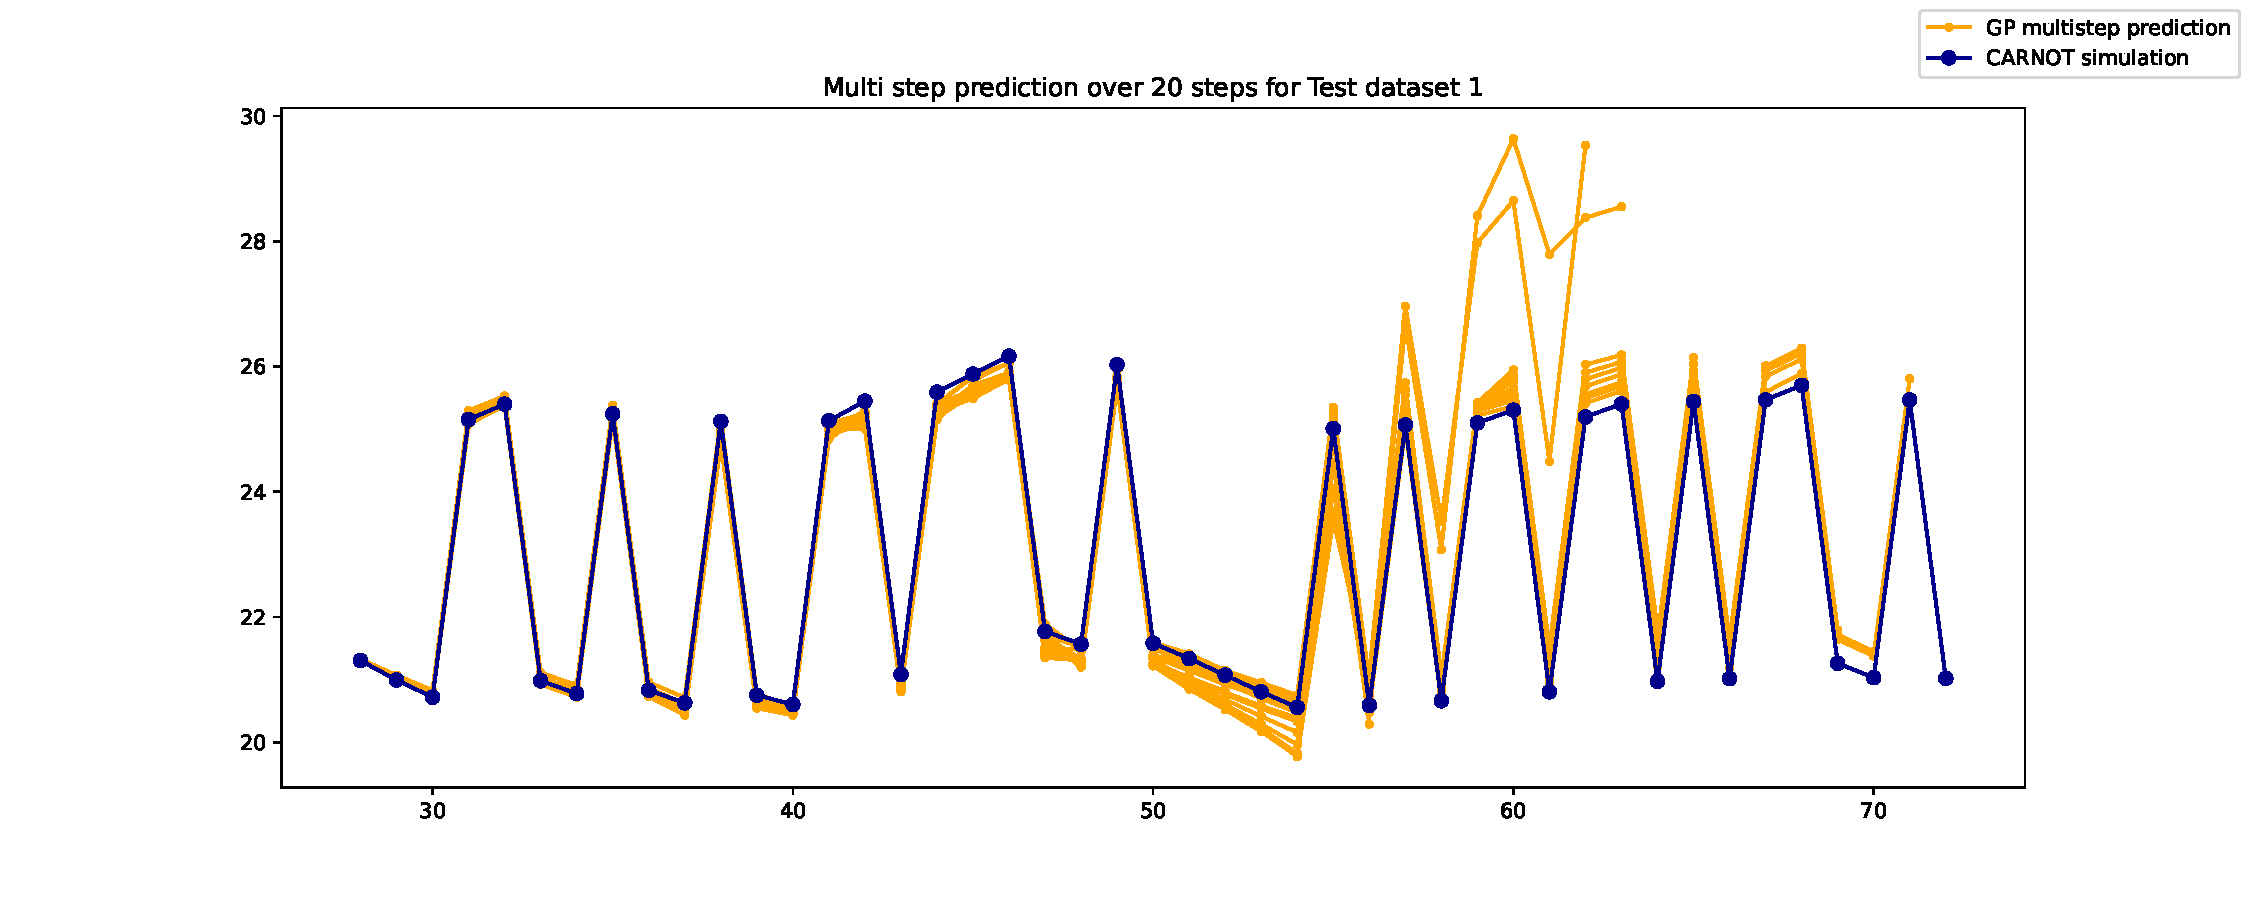
\includegraphics[width =
    \textwidth]{Plots/GP_213_-1pts_test_prediction_20_steps.pdf}
    \vspace{-25pt}
    \caption{20-step ahead simulation for \model{2}{1}{3}}
    \label{fig:GP_213_multistep_validation}
\end{figure}

The more complex model, presented in
Figure~\ref{fig:GP_213_multistep_validation} has a much better prediction
performance, with only two predictions out of a total of twenty five diverging
at the later steps. Except for the late-stage divergence on the two predictions,
this proves to be the best simulation model.

\begin{figure}[ht]
    \centering
    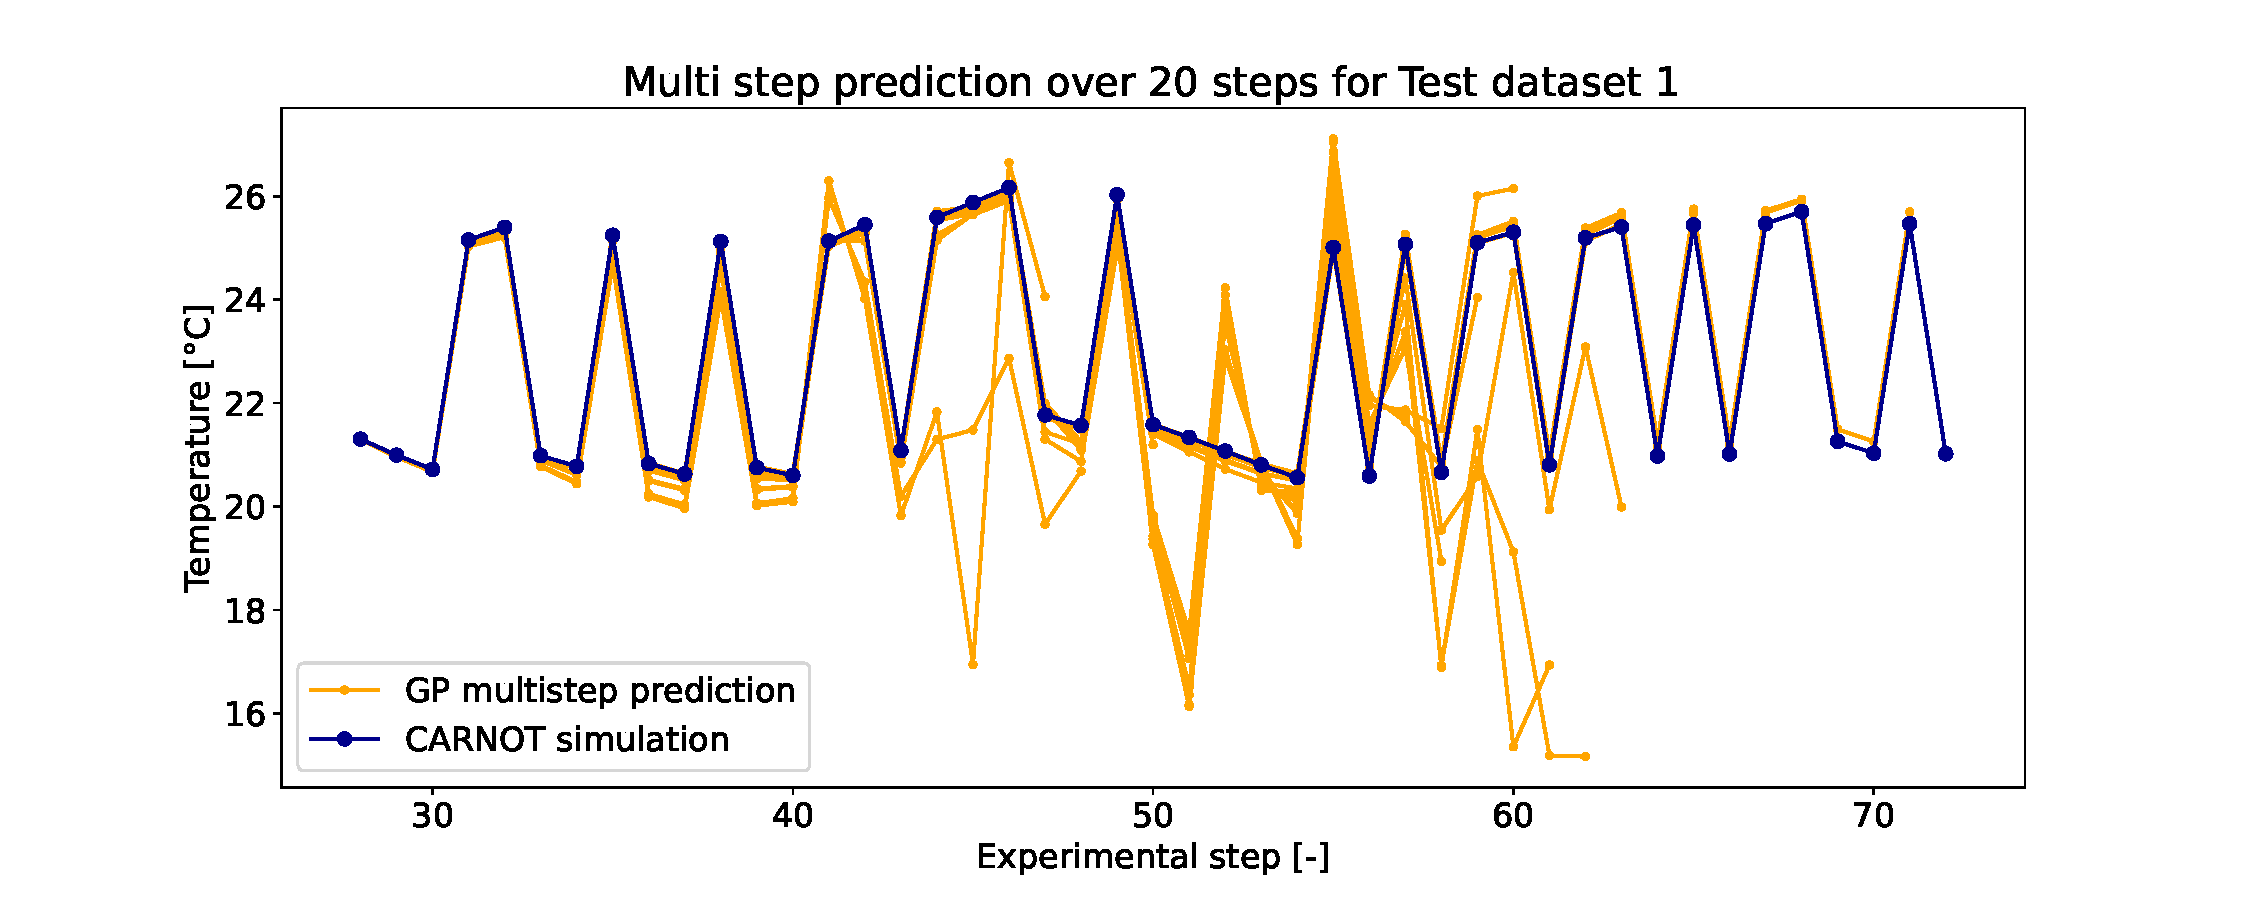
\includegraphics[width =
    \textwidth]{Plots/GP_313_-1pts_test_prediction_20_steps.pdf}
    \vspace{-25pt}
    \caption{20-step ahead simulation for \model{3}{1}{3}}
    \label{fig:GP_313_multistep_validation}
\end{figure}

Lastly, \model{3}{1}{3} has a much worse simulation performance than the other
two models. This could hint at an over fitting of the model on the training data.
This is consistent with the results found in Table~\ref{tab:GP_loss_functions}
for the \acrshort{rmse} and \acrshort{smse}, as well as can be seen in
Appendix~\ref{apx:hyperparams_gp}, Figure~\ref{fig:GP_313_test_validation},
where the model has much worse performance on the testing dataset predictions
than the other two models.

Overall, the performance of the three models in simulation mode is consistent
with the previously found results. It is of note that neither the model that
performed the best on the \acrshort{rmse}/\acrshort{smse}, \model{1}{2}{3}, nor
the one that had the best \acrshort{msll}/\acrshort{lpd}, perform the best under
a simulation scenario. In the case of the former it is due to numerical
instability, the training/ prediction often failing depending on the inputs. On
the other hand, in the case of the latter, only focusing on the
\acrshort{msll}/\acrshort{lpd} performance metrics can lead to over fitted
models, that give good and confident one-step ahead predictions, while still
unable to fit the true behaviour of the plant.

\clearpage

    \subsubsection{Sparse and Variational Gaussian Process}

For the \acrshort{svgp} models, only the performance of \model{1}{2}{3} was
investigated, since it had the best performance according to all four loss
metrics. 

As a first validation step, it is of note that the \acrshort{svgp} model was
able to accurately reproduce the training dataset with only 150 inducing
locations (cf.  Appendix~\ref{apx:hyperparams_svgp}). It also performs about as
well as the better \acrshort{gp} models for the one step prediction on the
testing datasets.

In the case of the simulation performance, presented in
Figure~\ref{fig:SVGP_multistep_validation}, two things are of particular
interest. First, all 25 simulations have good overall behaviour --- there are no
simulations starting to exhibit erratic behaviour --- this is a good indicator
for lack of over fitting. This behaviour is indicative of a more conservative
model than the ones identified for the \acrshort{gp} models. It is also possible
to conclude that given the same amount of data, the classical \acrshort{gp}
models can better learn plant behaviour, provided the correct choice of
regressors.

\begin{figure}[ht]
    \centering
    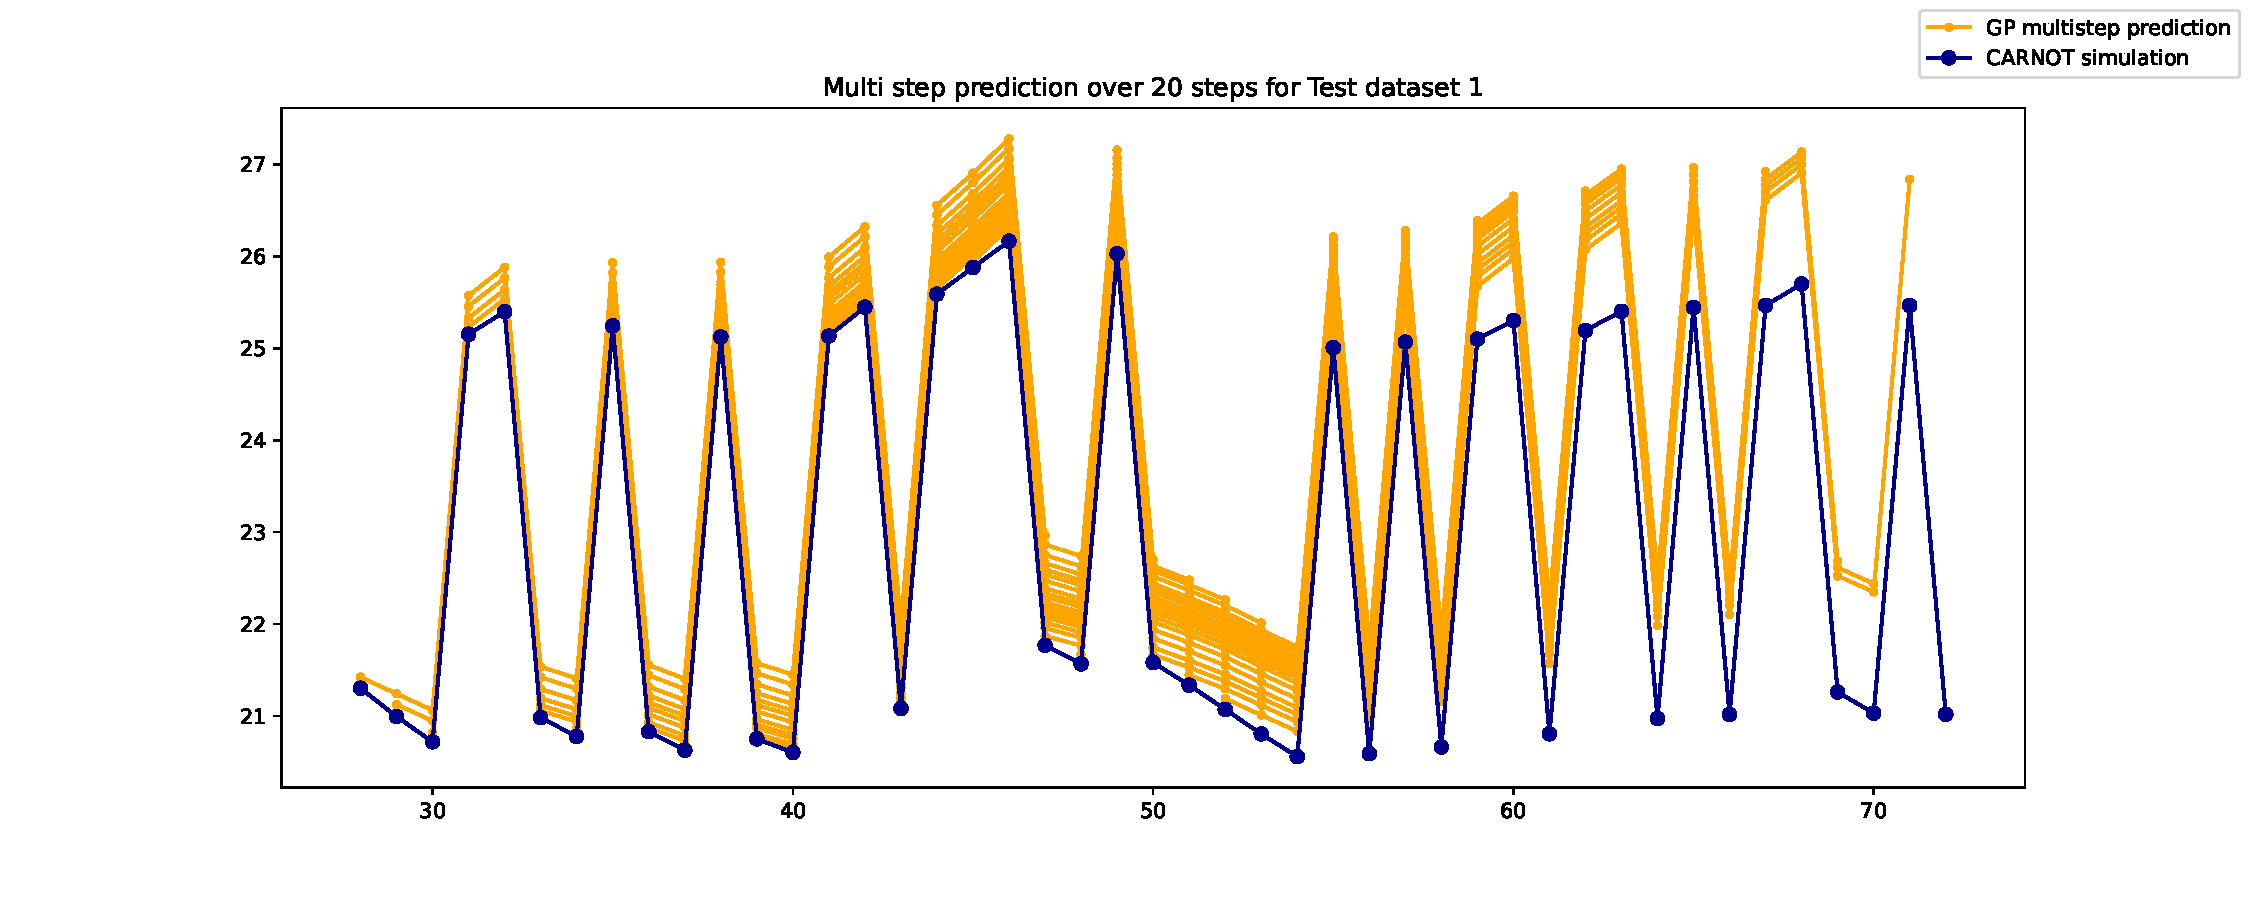
\includegraphics[width =
    \textwidth]{Plots/SVGP_123_test_prediction_20_steps.pdf}
    \caption{20-step ahead simulation for \model{1}{2}{3}}
    \label{fig:SVGP_multistep_validation}
\end{figure}


\clearpage

\section{The MPC Problem}\label{sec:mpc_problem}

The \acrlong{ocp} to be solved was chosen in such a way as to make
analysis of the models' performances more straightforward. The objective is
tracking a defined reference temperature as close as possible, while ensuring
the heat input stays within the HVAC capacity. The \textit{zero-variance} method
is used for multi-step prediction when using an existing \acrshort{gp}. This
does ignore the propagation of uncertainty for multi step ahead prediction, but
even with its simplicity, this method has been proven to work
~\cite{kocijanModellingControlDynamic2016,jainLearningControlUsing2018,
pleweSupervisoryModelPredictive2020}.

The optimization problem is therefore defined as follows:

\begin{subequations}\label{eq:optimal_control_problem}
    \begin{align}
        & \text{minimize}
        & & \sum_{i=0}^{N-1} (\bar{y}_{t+i} - y_{ref, t})^2 \\
        & \text{subject to}
        & & \bar{y}_{t+i} = K_*K^{-1}\mathbf{x}_{t+i-1} \\
        &&& \mathbf{x}_{t+i-1} = \left[\mathbf{w}_{t+i-1},\quad
        \mathbf{u}_{t+i-1},\quad \mathbf{y}_{t+i-1}\right]^T \\
        \label{eq:components}
        &&& u_{t+i} \in \mathcal{U}
    \end{align}
\end{subequations}

where $y_{ref, t}$ is the reference temperature at time t, $\mathbf{x}_{t}$ is
the GP input vector at time t, composed of the exogenous autoregressive inputs
$\mathbf{w}_{t}$, the autoregressive controlled inputs $\mathbf{u}_{t}$ and the
autoregressive outputs $\mathbf{y}_{t}$.

\subsection{Temperature reference}\label{sec:reference_temperature}

The temperature reference for the controller has been taken as the mean value of
the SIA~180:2014~\cite{sia180:2014ProtectionThermiqueProtection2014} temperature
norm. It imposes a range of temperatures that are allowed for residential
buildings based on the rolling 48h average outside temperature.


\begin{figure}[ht]
    \centering
    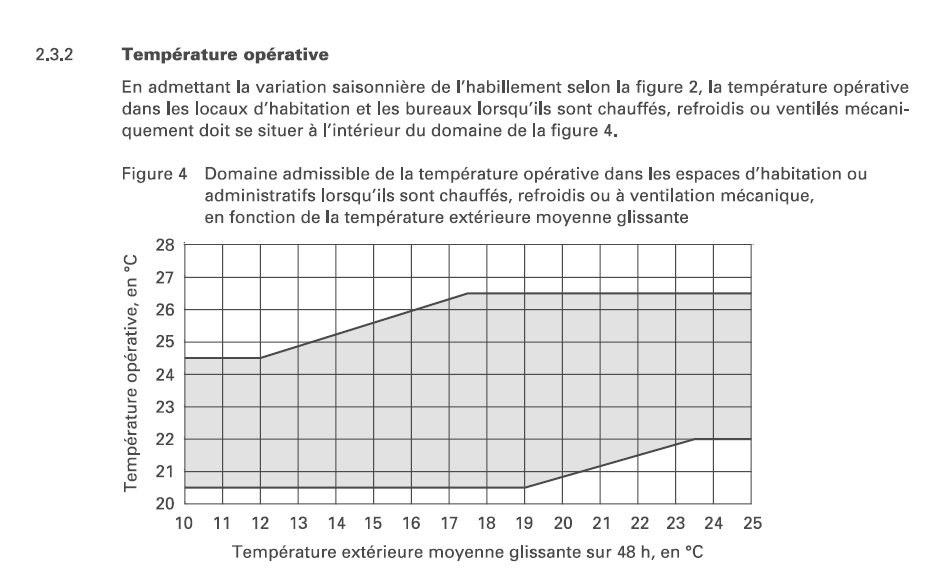
\includegraphics[width = \textwidth]{Images/sia_180_2014.png}
    \caption{The SIA 180:2014 norm for residential building temperatures}
    \label{fig:sia_temperature_norm}
\end{figure}

\clearpage

\section{Implementation}


\begin{figure}[ht]
    \centering
    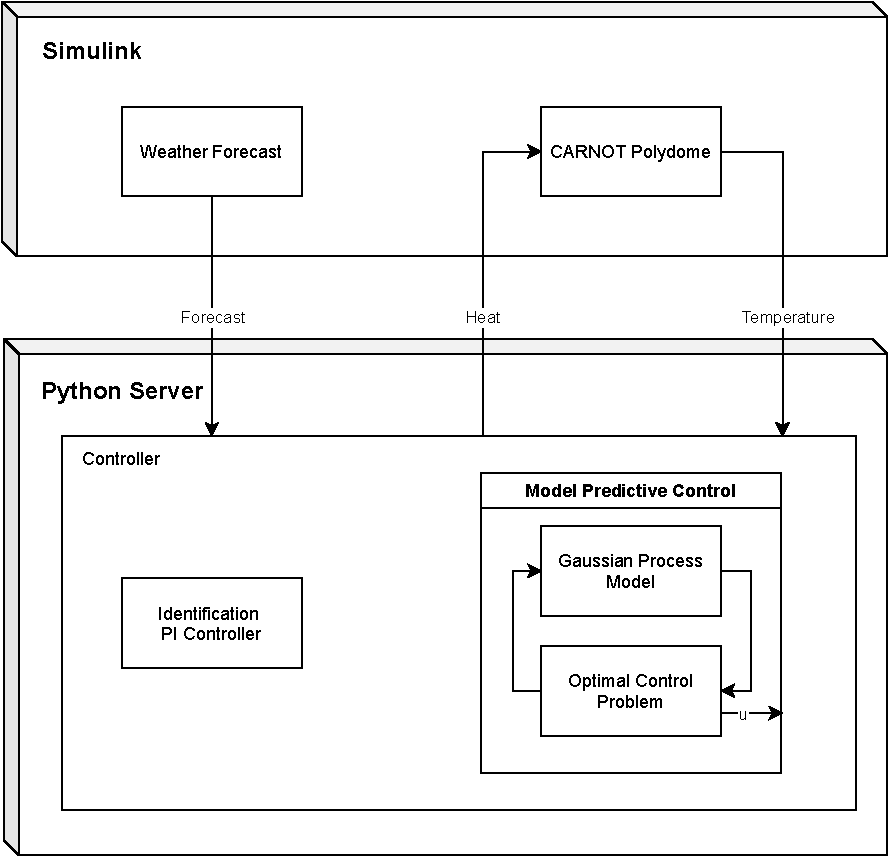
\includegraphics[width = 0.5\textwidth]{Images/setup_diagram.pdf}
    \caption{Block diagram of the Simulink plant and Python Controller}
    \label{fig:setup_diagram}
\end{figure}


% TODO: [Implementation] Reference implementation details for CARNOT and WDB

\subsection{Gaussian Processes}

% TODO: [Implementation] Cite Tensorflow
% TODO: [Implementation] Cite GPflow

\subsection{Classical Gaussian Process training}
\subsection{Sparse and Variational Gaussian Process training}


\subsection{Optimal Control Problem}
\subsubsection{Sparse Implementation of the Optimization Problem}

The optimization problem as presented in
Equation~\ref{eq:optimal_control_problem} becomes very nonlinear quite fast. In
fact, due to the autoregressive structure of the \acrshort{gp}, the predicted
temperature at time t is passed as an input to the model at time $t+1$. A simple
recursive implementation of the Optimization Problem becomes untractable after
only 3 --- 4 prediction steps. 

In order to solve this problem, a new OCP is introduced. It has a much sparser
structure, in exchange for a larger number of variables. This turns out to be
much faster to solve than the original problem.

Let $w_l$, $u_l$, and $y_l$ be the lengths of the state vector components
$\mathbf{w}$, $\mathbf{u}$, $\mathbf{y}$ (cf. Equation~\ref{eq:components}).

\begin{subequations}\label{eq:sparse_optimal_control_problem}
    \begin{align}
        & \text{minimize}
        & & \sum_{i=2}^{N + 1} \left(X[i, w_l + u_l + 1] - y_{ref, t}\right)^2 \\
        & \text{subject to}
        & & X[i+1, w_l + u_l + 1] = K_*K^{-1}X[i, :] \quad \text{for} \quad
        i\in[1, N]\\
        &&& X[i, w_l + u_l + 2: ] = X[i, w_l+ u_l + 1: w_l + u_l + y_l - 1]\\
        &&& X[i, 1:w_l] = W[i, :] \\
        &&& X[i+1, w_l + 2: w_l + u_l] = X[i, w_l + 1: w_l + u_l - 1] \\
        &&& X[:, w_l + 1] \in \mathcal{U}
    \end{align}
\end{subequations}

where X is the matrix of all the system states and W is the matrix of the
disturbances.

\subsubsection{RENAME: Python implementation of the control problem}
% TODO: [Implementation] Cite CasADi
% TODO: [Implementation] Cite HSL solvers for using MA27


\subsection{Python server and controller objects}


\clearpage

\section{Results}\label{sec:results}


% TODO [Results] Add info on control horizon

This section focuses on the presentation and interpretation of the year-long
simulation of the control schemes present previously.

Section~\ref{sec:GP_results} analyses the results of a conventional
\acrlong{gp} Model trained on the first five days of gathered data. The models
is then used for the rest of the year, with the goal of tracking the defined
reference temperature.

Section~\ref{sec:SVGP_results} goes into details on the analysis of the Learning
scheme using a \acrshort{svgp} Model. In this scenario, the model is first
trained on the first five days of data, and updates every day at midnight with
the new information gathered from closed-loop operation.

\subsection{Conventional Gaussian Processes}\label{sec:GP_results}

The first simulation, to be used as a baseline comparison with the
\acrshort{svgp} Models developed further consists of using a `static'
\acrshort{gp} model trained on five days worth of experimental data. This model
is then employed for the rest of the year.

With a sampling time of 15 minutes, the model is trained on 480 points of data.
This size of the identification dataset is enough to learn the behaviour of the
plant, without being too complex to solve from a numerical perspective, the
current implementation takes roughly 1.5 seconds of computation time per step.
For reference, identifying a model on 15 days worth of experimental data (1440
points) makes simulation time approximately 11 --- 14 seconds per step, or
around eight time slower. This is consistent with the $\mathcal{O}(n^3)$
complexity of evaluating a \acrshort{gp}.

The results of the simulation are presented in
Figure~\ref{fig:GP_fullyear_simulation}. Overall, the performance of this model
is not very good. The tracked temperature presents an offset of around 0.5
$\degree$C in the stable part of the simulation. The offset becomes much larger
once the reference temperature starts moving from the initial constant value.
The controller becomes completely unstable around the middle of July, and can
only regain some stability at the middle of October. It is also possible to note
that from mid-October --- end-December the controller has very similar
performance to that exhibited in the beginning of the year, namely January ---
end-February.

\begin{figure}[ht]
    \centering
    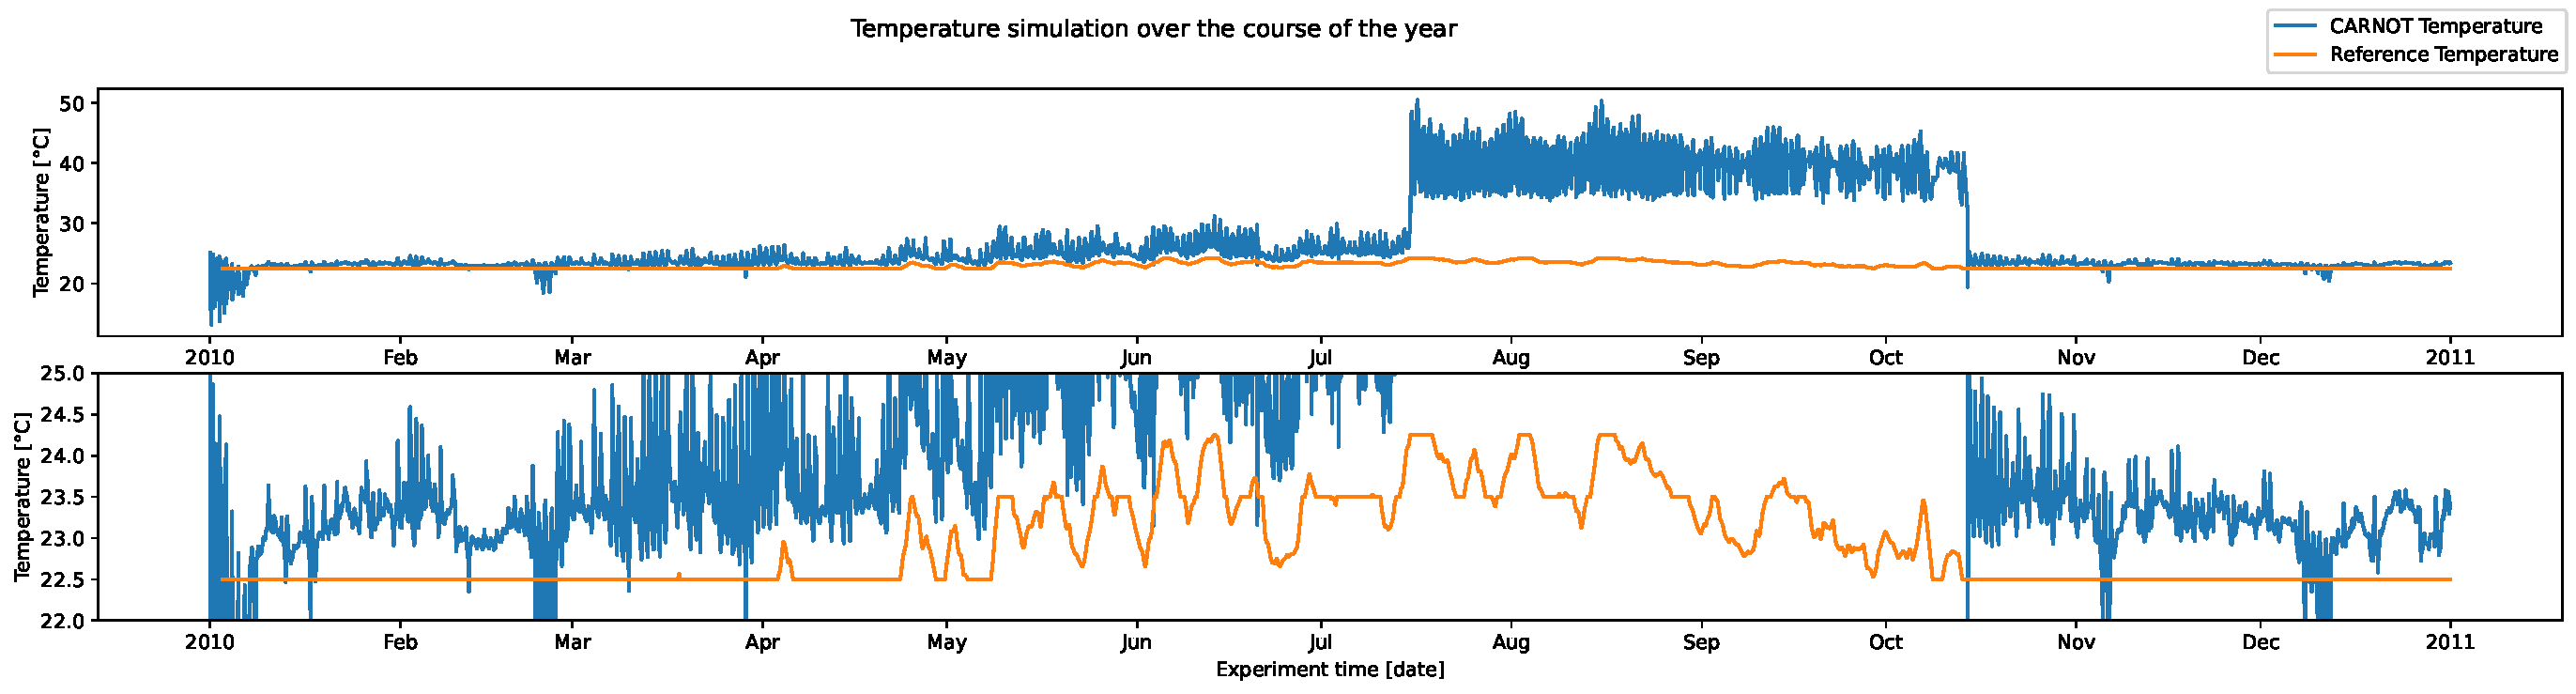
\includegraphics[width =
    \textwidth]{Plots/4_GP_480pts_12_averageYear_fullyear.pdf}
    \caption{GP full year simulation}
    \label{fig:GP_fullyear_simulation}
\end{figure}

This very large difference in performance could be explained by the change in
weather during the year. The winter months of the beginning of the year and end
of year exhibit similar performance, the spring months already make the
controller less stable than at the start of the year, while the drastic
temperature changes in the summer make the controller completely unstable.

\clearpage


Figure~\ref{fig:GP_fullyear_abserr} presents the absolute error measured at each
step of the simulation over the course of the year. We can note a mean absolute
error of 1.33 $\degree$C, with the largest deviations occurring in late summer
where the absolute error can reach extreme values, and the `best' performance
occurring during the winter months. 

\begin{figure}[ht]
    \centering
    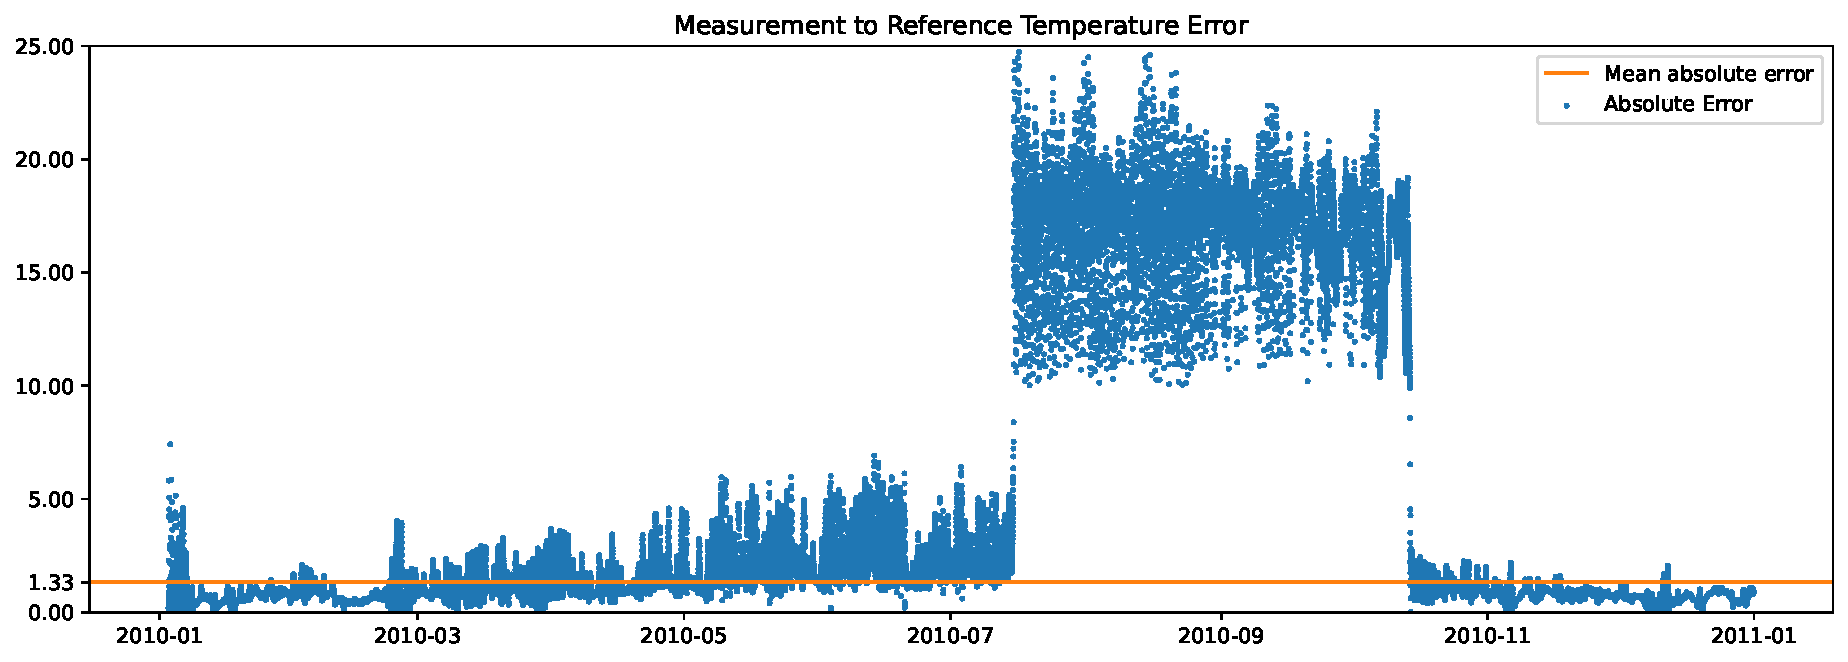
\includegraphics[width =
    \textwidth]{Plots/4_GP_480pts_12_averageYear_abserr.pdf}
    \caption{GP full year absolute error}
    \label{fig:GP_fullyear_abserr}
\end{figure}

Figure~\ref{fig:GP_first_model_performance} analyses the 20-step ahead
simulation performance of the identified model over the course of the year. At
experimental step 250 the controller is still gathering data. It is therefore
expected that the identified model will be capable of reproducing this data. At
step 500, 20 steps after identification, the model correctly steers the internal
temperature towards the reference temperature. On the flip side, already at
experimental steps 750 and 1000, only 9 days into the simulation, the model is
unable to properly simulate the behaviour of the plant, with the maximum
difference at the end of the simulation reaching 0.75 and 1.5 $\degree$C
respectively.

\begin{figure}[ht]
    \centering
    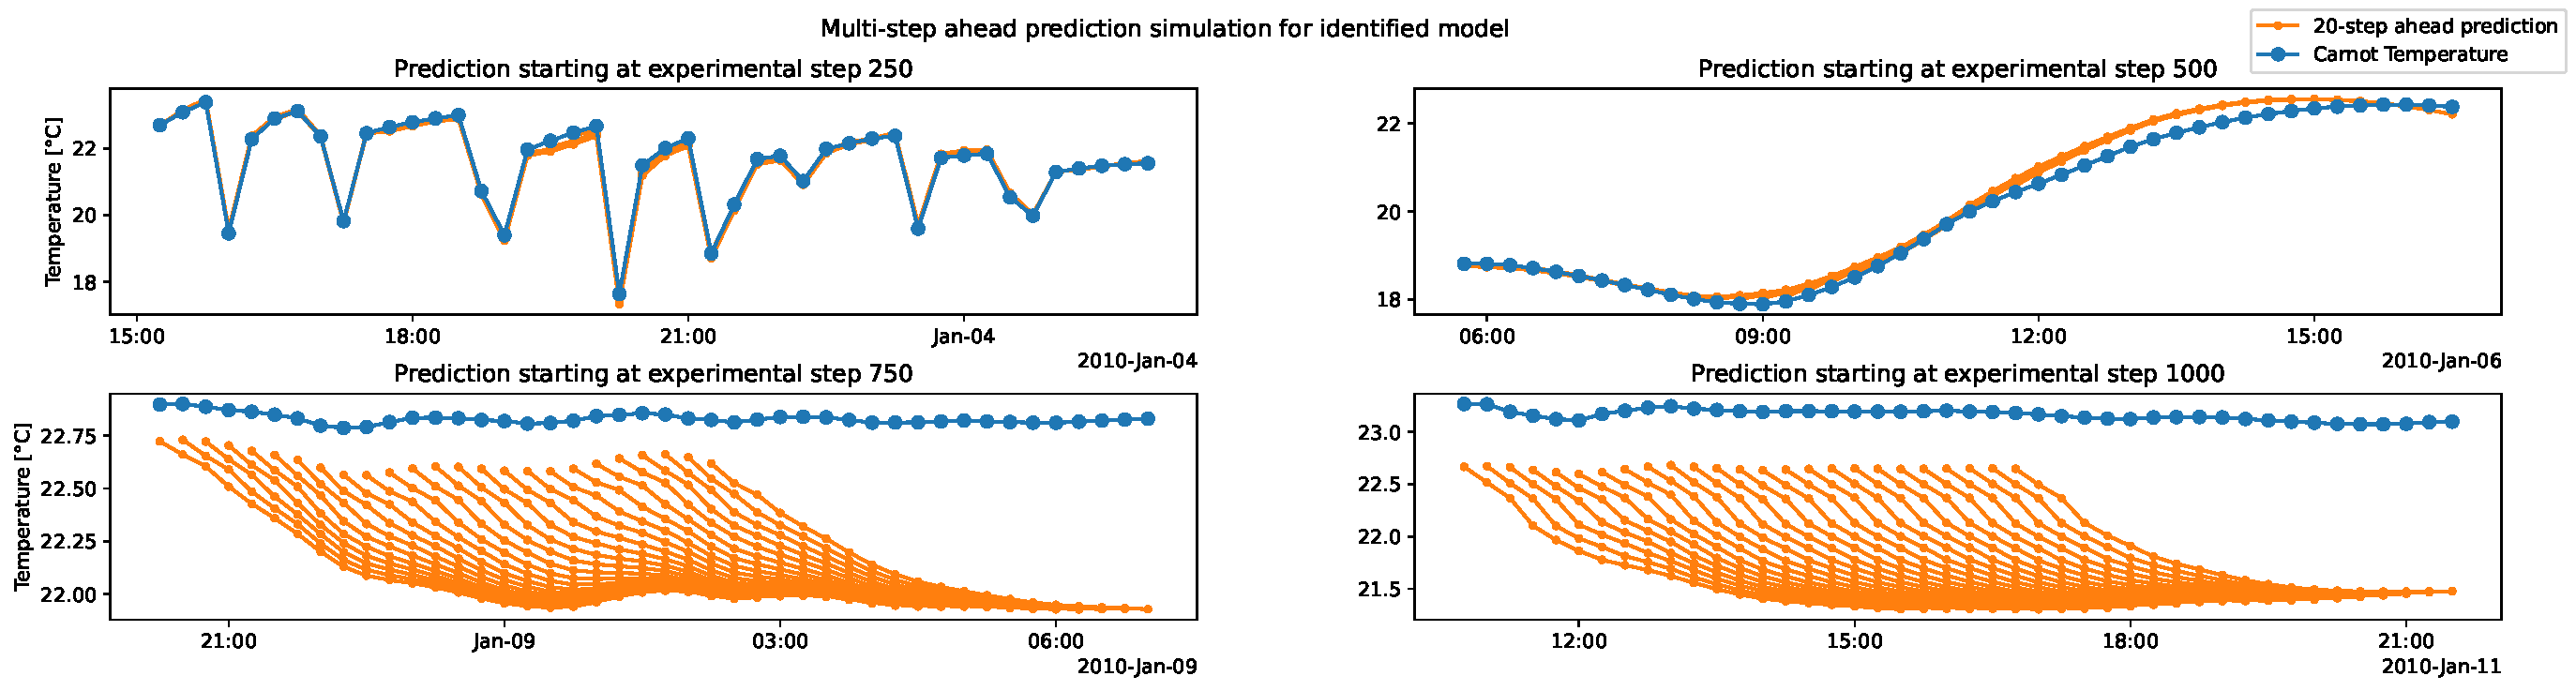
\includegraphics[width =
    \textwidth]{Plots/4_GP_480pts_12_averageYear_first_model_performance.pdf}
    \caption{GP model performance}
    \label{fig:GP_first_model_performance}
\end{figure}

This large difference of performance could be explained by the change in outside
weather (Solar Irradiance and Outside Temperature --- the exogenous inputs) from
the one present during the training phase. It can be seen in
Figure~\ref{fig:Dataset_outside_temperature} that already at 500 points in the
simulation both the GHI and the Outside Temperature are outside of the training
ranges, with the latter exhibiting a much larger variation. 


\begin{figure}[ht]
    \centering
    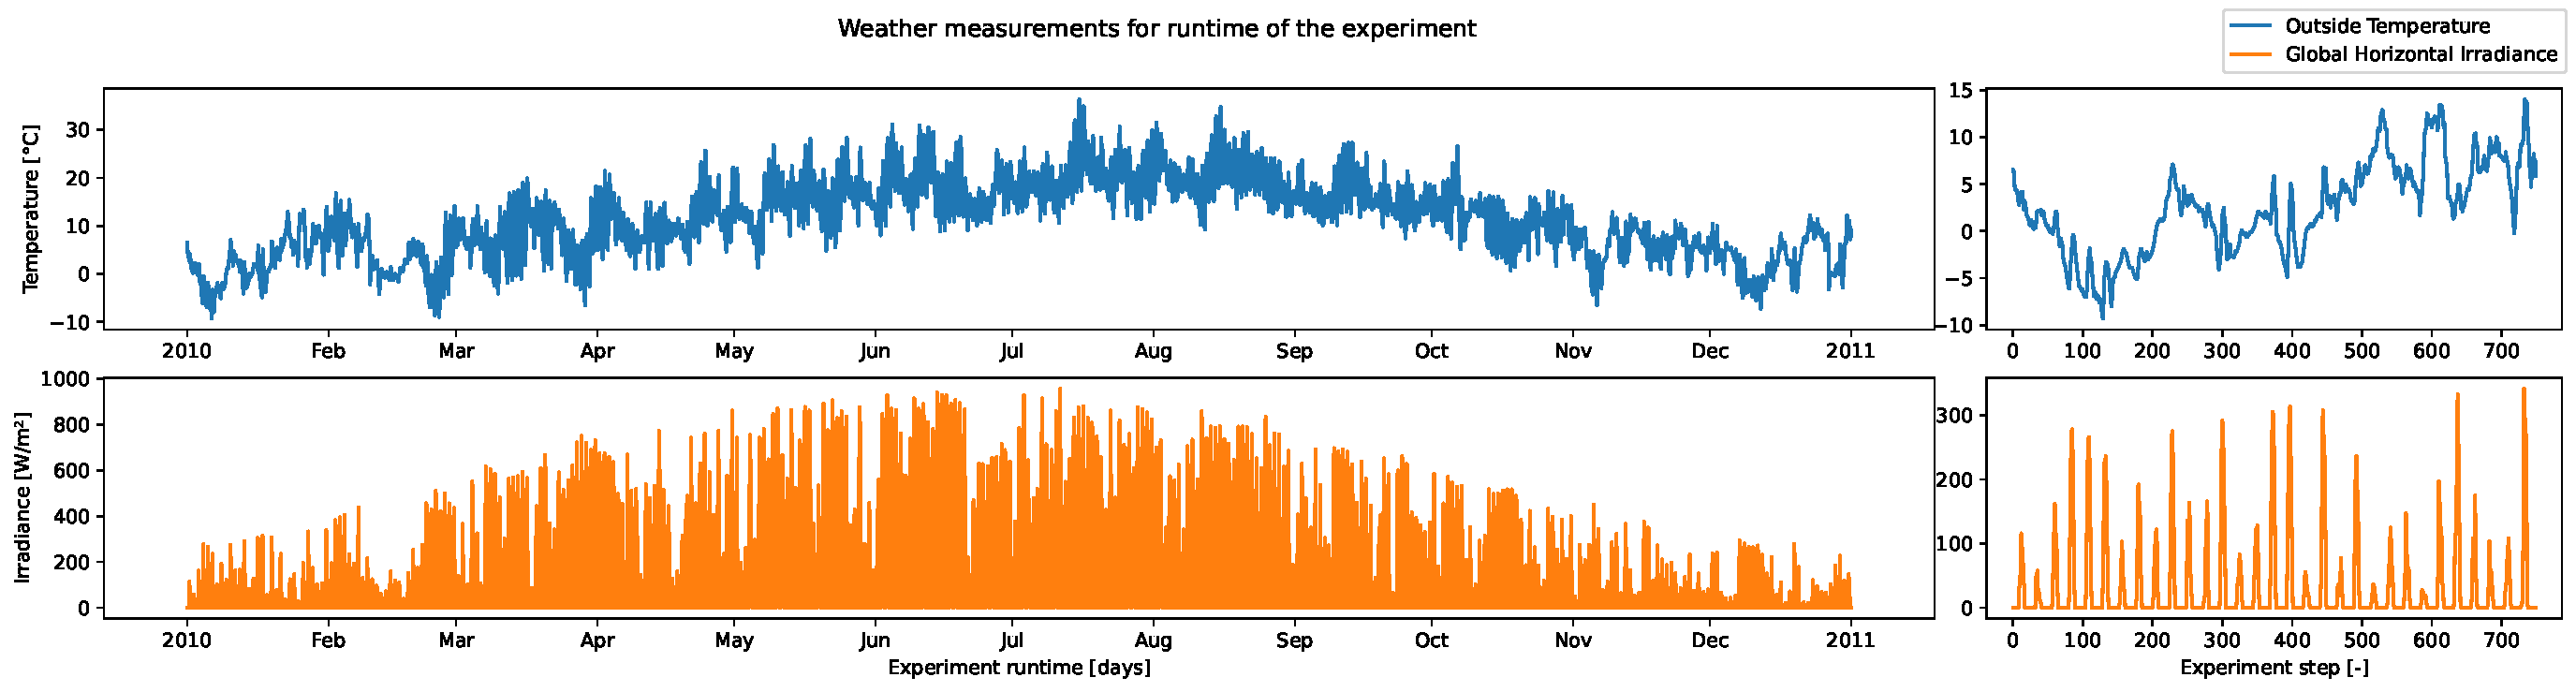
\includegraphics[width =
    \textwidth]{Plots/Exogenous_inputs_fullyear.pdf}
    \caption{Exogenous inputs for the simulation}
    \label{fig:Dataset_outside_temperature}
\end{figure}

Finally, it is possible to conclude that this approach does not perform well due
to several causes:

\begin{itemize}
    \item The size of the training dataset is limited by the computation budget
    \item The model does not extrapolate correctly the information on
        disturbances
    \item The model stays fixed for the duration of the year, being unable to
        adapt to new weather conditions.
\end{itemize}

These problems could be solved in several ways, such as periodically
re-identifying the model to fit the current weather pattern. This approach would
be quite cumbersome due to repeated need of disturbing the model in order to
sufficiently excite it. Another approach would be to keep the whole historical
dataset of measurements, which quickly renders the problem intractable. More
complex solutions, such as keeping a fixed-size data dictionary whose points are
deleted when they no longer help the predictions and new points are added as
they are deemed useful or compiling the training dataset with multiple
experiments in different weather conditions could dramatically improve model
performance, but are more complex in implementation.


\subsection{Sparse and Variational Gaussian Process}\label{sec:SVGP_results}

The \acrlong{svgp} models are setup in a similar way as described before. The
model is first identified using 5 days worth of experimental data collected
using a \acrshort{pi} controller and a random disturbance signal. The difference
lies in the fact than the \acrshort{svgp} model gets re-identified every night
at midnight using the newly accumulated data from closed-loop operation.

The results of this setup are presented in
Figure~\ref{fig:SVGP_fullyear_simulation}. It can already be seen that this
setup performs much better than the initial one. The only large deviations from
the reference temperature are due to cold --- when the \acrshort{hvac}'s limited
heat capacity is unable to maintain the proper temperature.

% TODO: [Results] Add info on SVGP vs GP computation speed

\begin{figure}[ht]
    \centering
    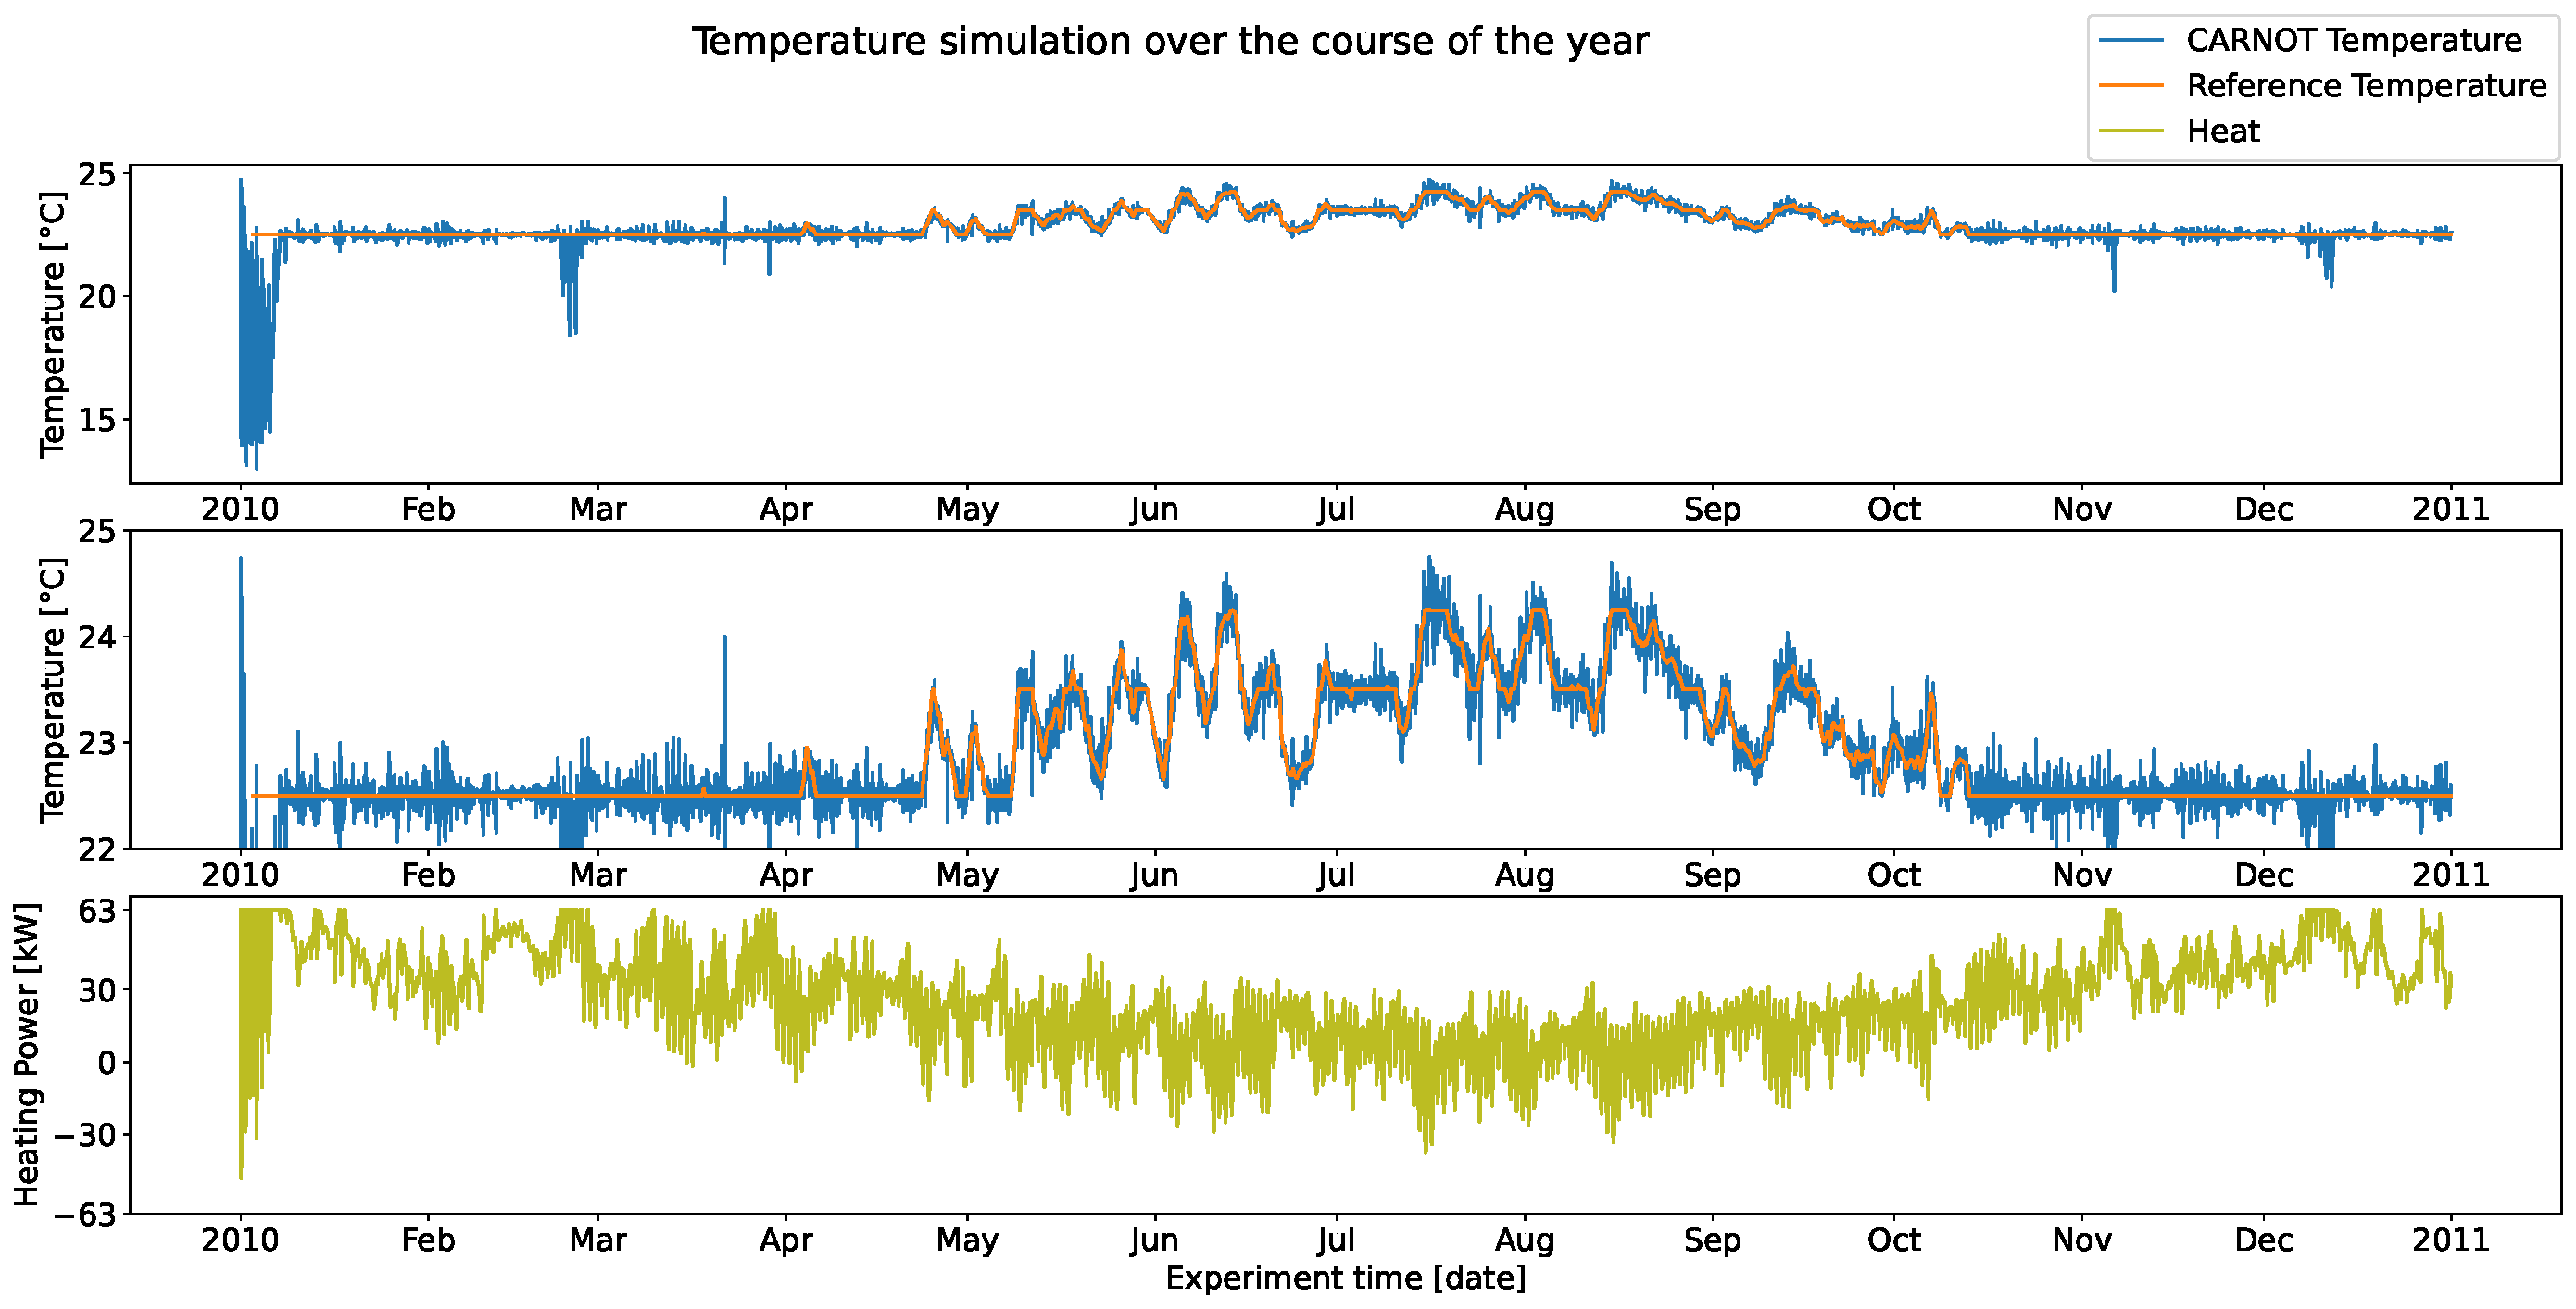
\includegraphics[width =
    \textwidth]{Plots/1_SVGP_480pts_inf_window_12_averageYear_fullyear.pdf}
    \caption{SVGP full year simulation}
    \label{fig:SVGP_fullyear_simulation}
\end{figure}

\clearpage

Comparing the Absolute Error of the Measured vs Reference temperature for the
duration of the experiment (cf. Figure~\ref{fig:SVGP_fullyear_abserr}) with the
one of the original experiment, the average absolute error is reduced from 1.33
$\degree$C to only 0.05 $\degree$C, with the majority of the values being lower
than 0.4 $\degree$ C. 

\begin{figure}[ht]
    \centering
    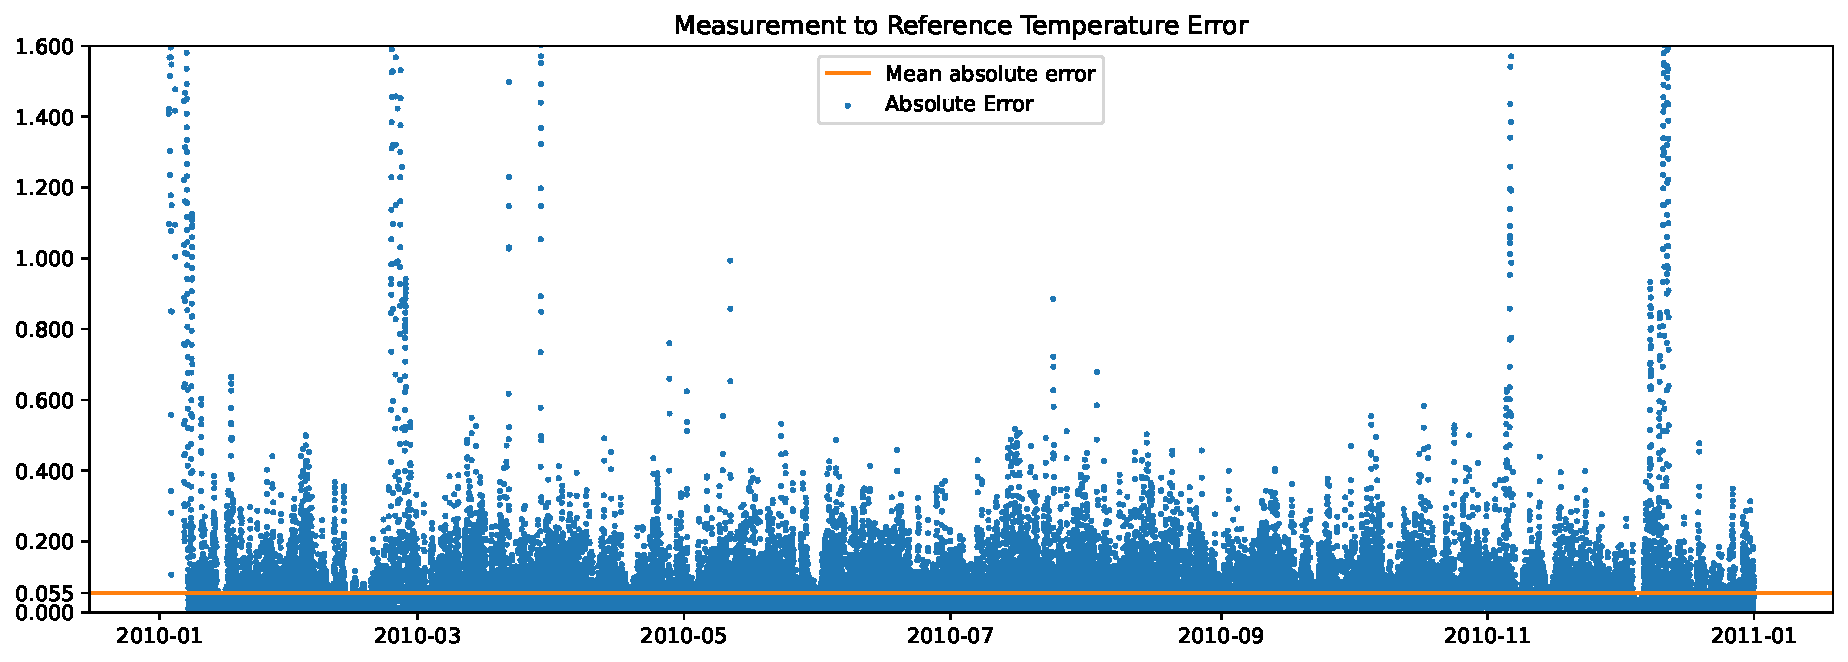
\includegraphics[width =
    \textwidth]{Plots/1_SVGP_480pts_inf_window_12_averageYear_abserr.pdf}
    \caption{SVGP full year absolute error}
    \label{fig:SVGP_fullyear_abserr}
\end{figure}

Figures~\ref{fig:SVGP_first_model_performance},
~\ref{fig:SVGP_later_model_performance}
and~\ref{fig:SVGP_last_model_performance} show the 20-step simulation performance of three
different models, identified at three different stages of the experiment. They
have all been set to simulate 25 consecutive experimental steps starting at
steps 250, 500, 10750 and 11000 respectively.

The initial model (cf. Figure~\ref{fig:SVGP_first_model_performance}),
identified after the first five days has the worst performance. It is unable to
correctly simulate even the learning dataset. This behaviour is similar to that
discovered in Figure~\ref{fig:SVGP_multistep_validation}
(cf. Section~\ref{sec:validation_hyperparameters}), where the \acrshort{svgp}
model performed worse than the equivalent \acrshort{gp} trained on the same
dataset. It also performs worse than the initial \acrshort{gp} model in the rest
of the simulations, being unable to correctly predict the heating to reference
at step 500, and having maximum errors of around 10 $\degree$C for the simulations
starting at 107500 and 11000 points.

\begin{figure}[ht]
    \centering
    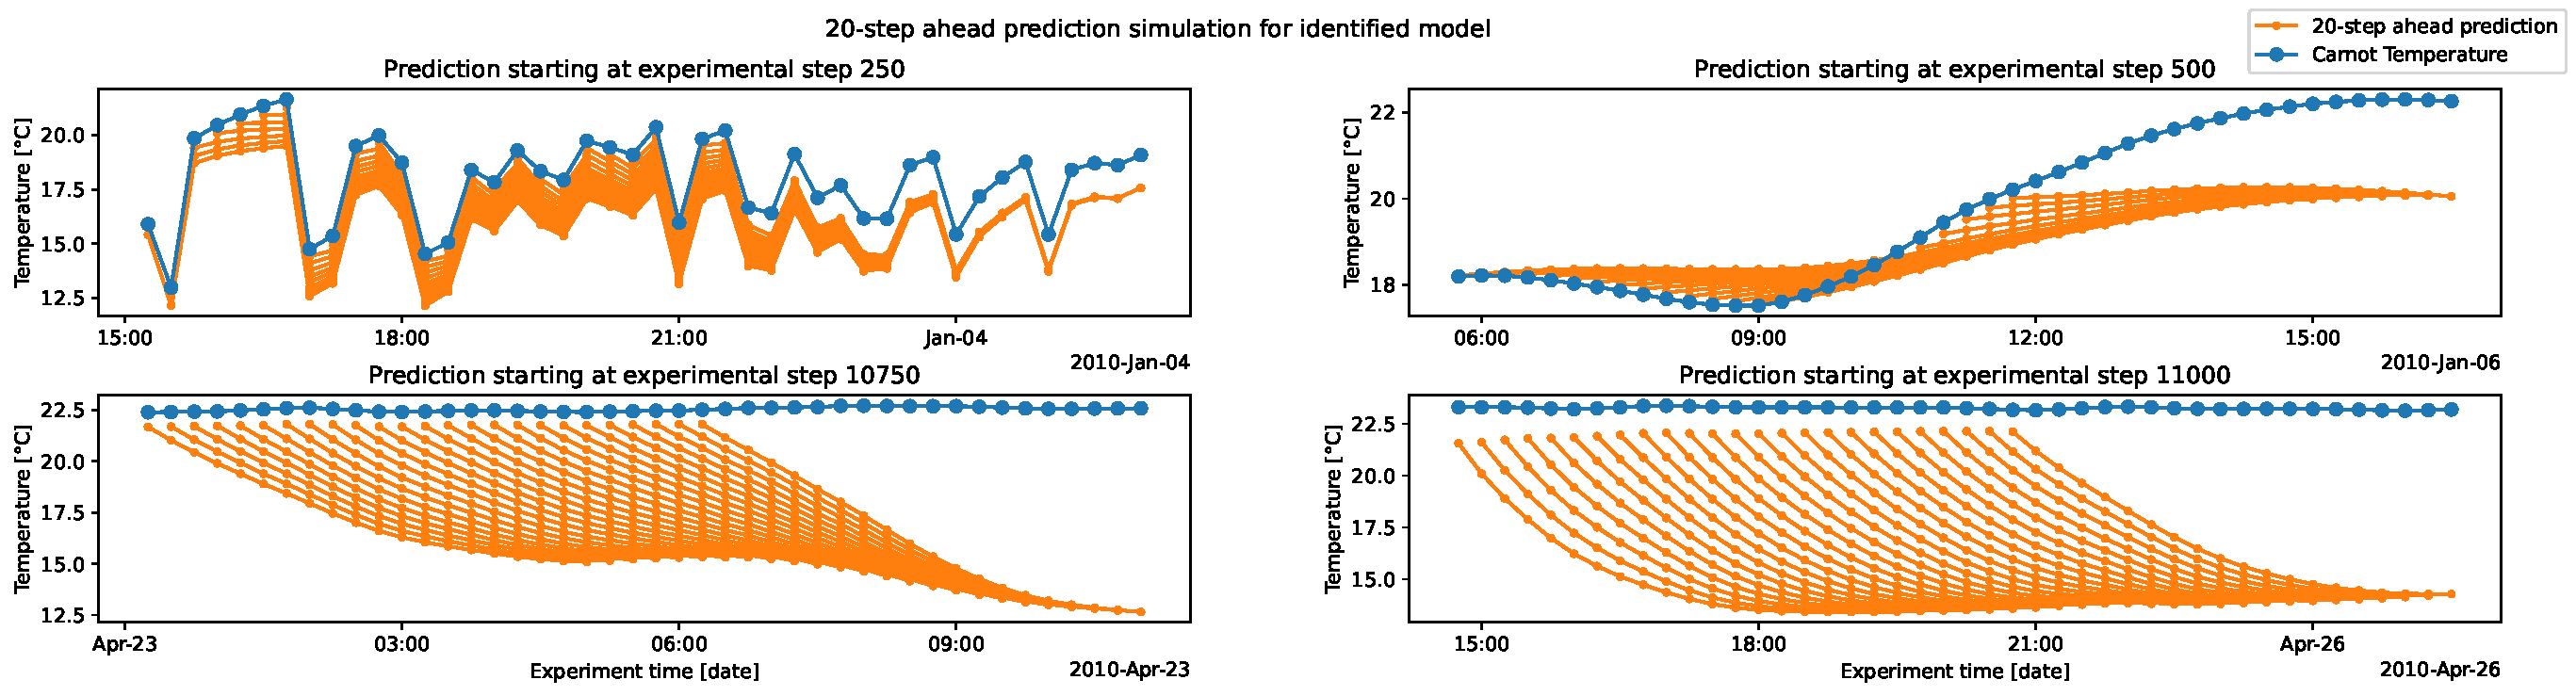
\includegraphics[width =
    \textwidth]{Plots/1_SVGP_480pts_inf_window_12_averageYear_first_model_performance.pdf}
    \caption{GP first model performance}
    \label{fig:SVGP_first_model_performance}
\end{figure}

\clearpage

Figure~\ref{fig:SVGP_later_model_performance} shows the performance of the 100th
trained model (i.e the model trained on April 15). This model performs much
better in all simulations. It is able to correctly simulate the 20-step
behaviour of the plant over all the experimental steps in the first two cases.
It still has a noticeable error when predicting the behaviour of the plant on
new data (i.e. simulations starting at steps 10750 and 11000), but it is much
less than before. This gives a hint at the fact that the \acrshort{svgp} model's
performance ameliorates throughout the year, but it does require much more data
than the classical \acrshort{gp} model to capture the building dynamics.

\begin{figure}[ht]
    \centering
    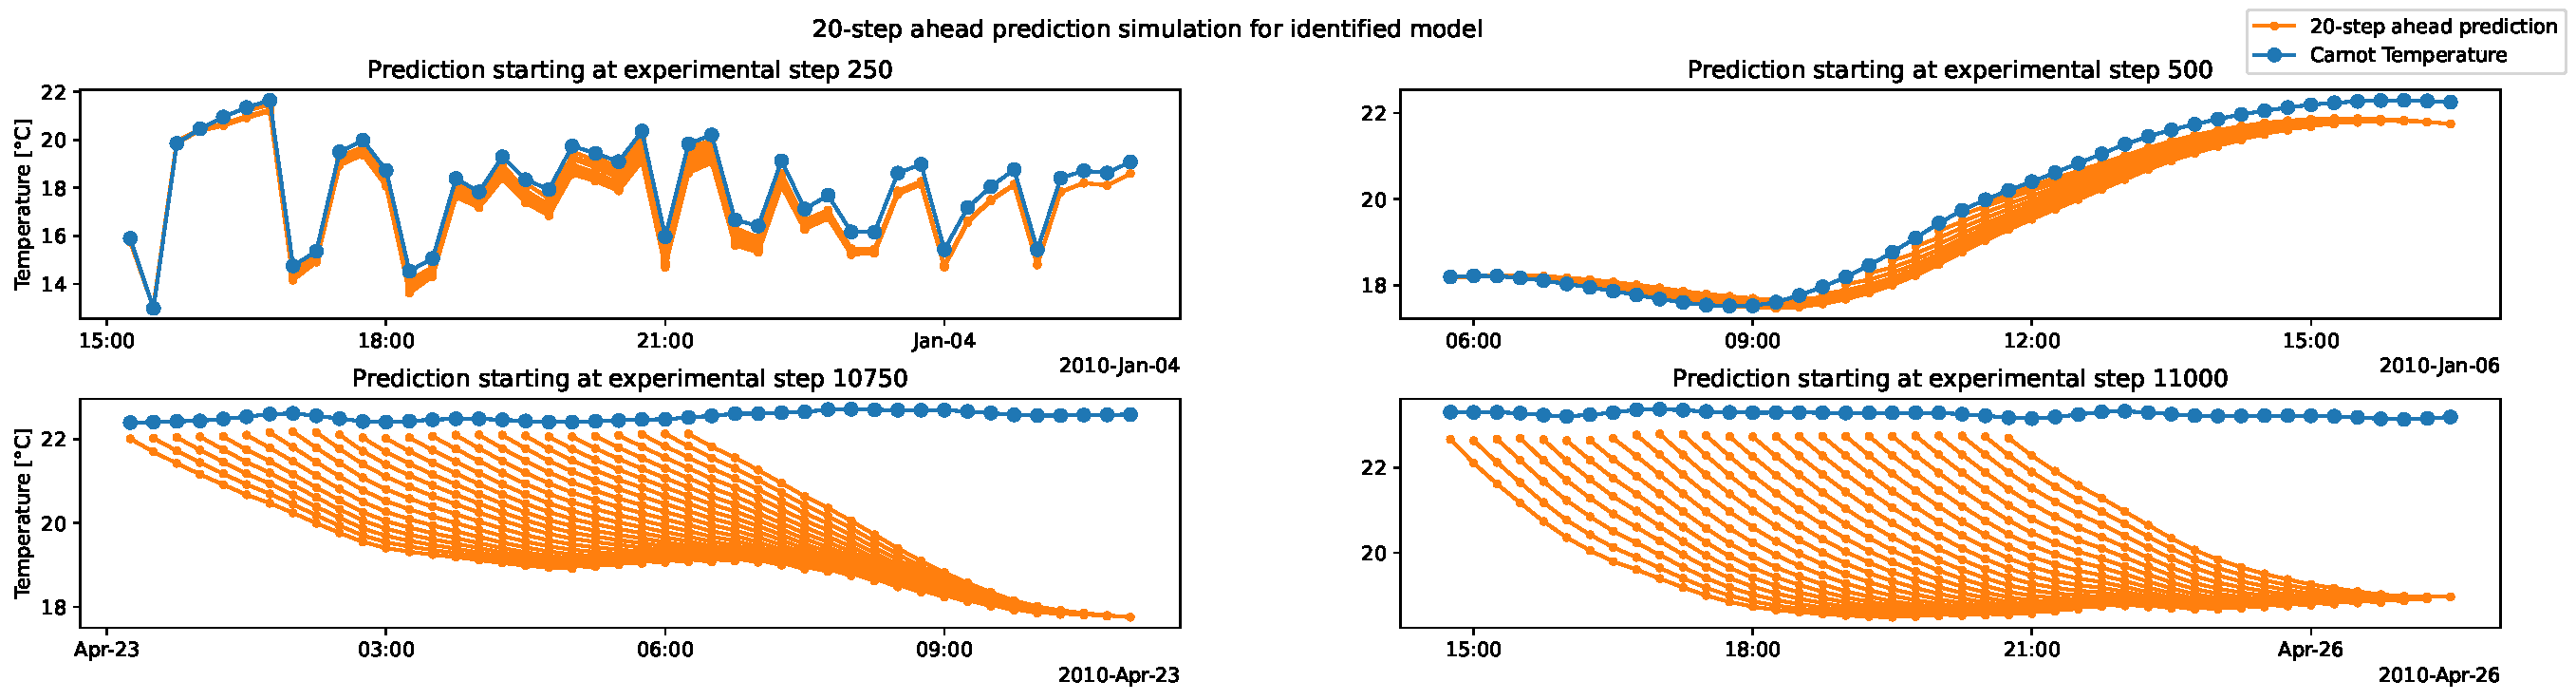
\includegraphics[width =
    \textwidth]{Plots/1_SVGP_480pts_inf_window_12_averageYear_later_model_performance.pdf}
    \caption{GP later model performance}
    \label{fig:SVGP_later_model_performance}
\end{figure}

The last model is trained on the whole-year dataset.
Figure~\ref{fig:SVGP_last_model_performance} shows its performance for the same
situation described before. The model is able to predict the plant's behaviour
at steps 250 and 500 even better than before, as well as predict the behaviour
at steps 10750 and 11000 with maximum error of 0.6 $\degree$C and 0.1 $\degree$C
respectively.

\begin{figure}[ht]
    \centering
    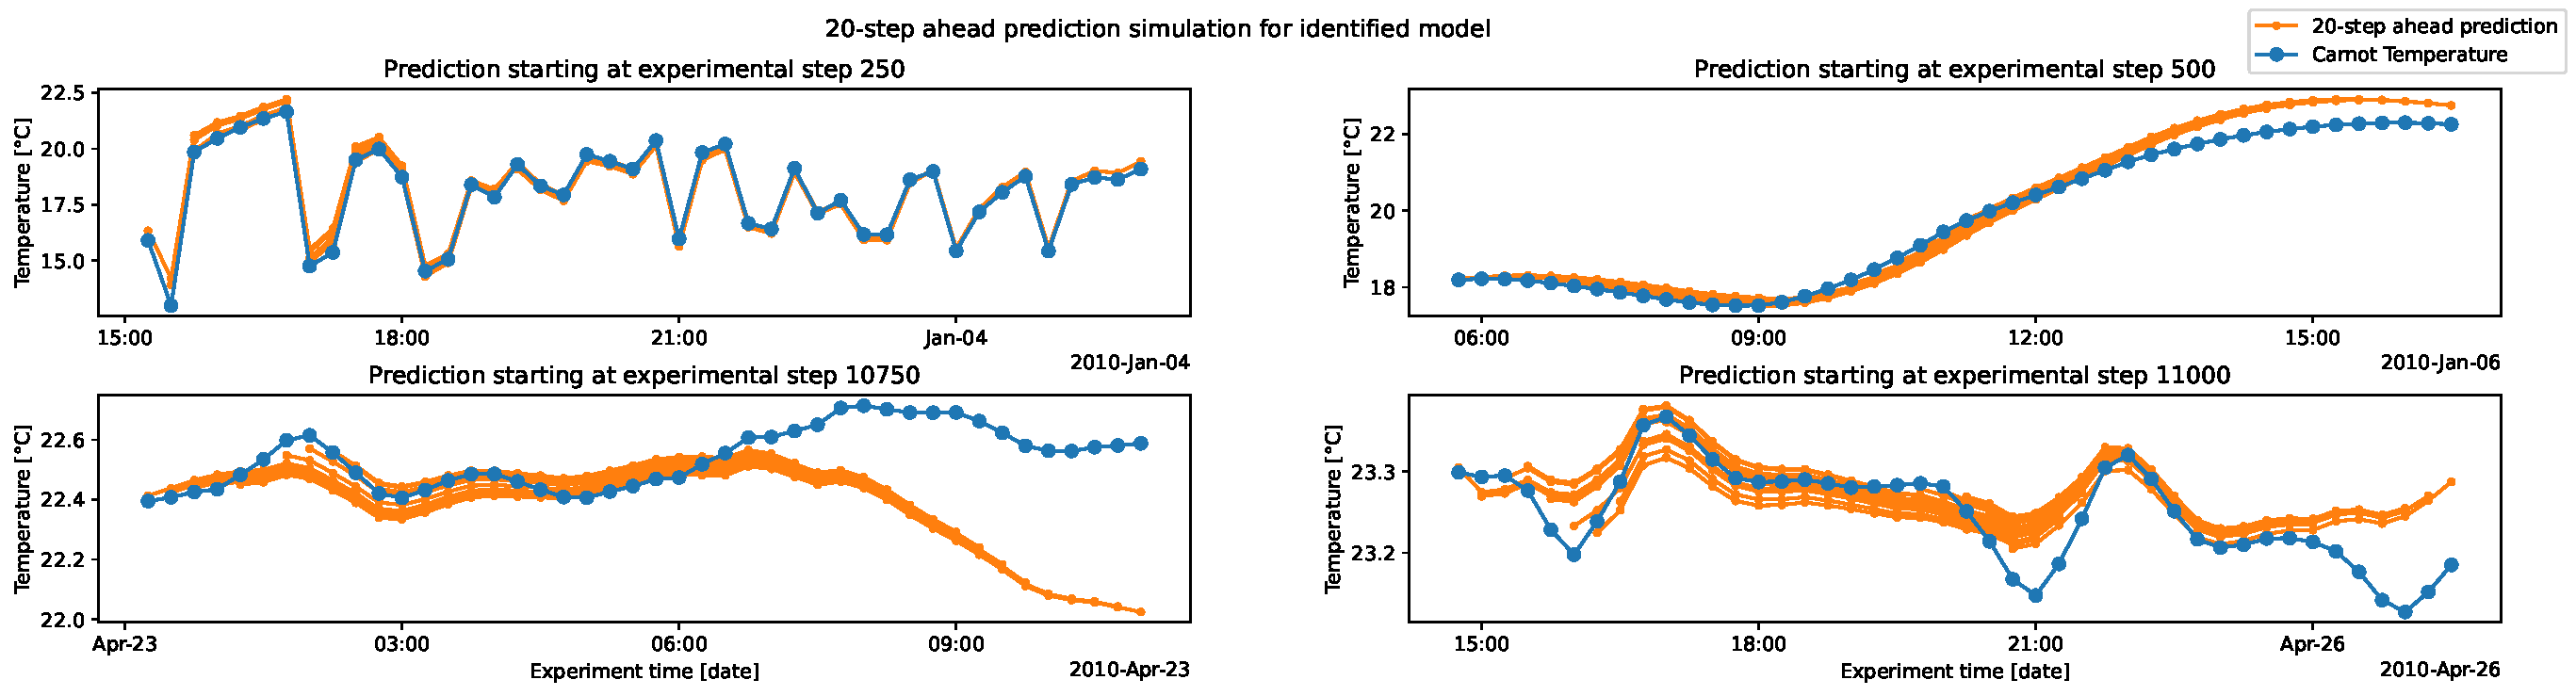
\includegraphics[width =
    \textwidth]{Plots/1_SVGP_480pts_inf_window_12_averageYear_last_model_performance.pdf}
    \caption{GP last model performance}
    \label{fig:SVGP_last_model_performance}
\end{figure}

The analysis of the model evolution as more data gets gathered already gives
very good insight into the strengths and weaknesses of this approach. The
initial model is unable to correctly extrapolate the plant's behaviour in new
regions of the state space. Also, given the same amount of data, the
\acrshort{svgp} model is able to capture less information about the plant
dynamics than the equivalent \acrshort{gp} model. On the flip side, re-training
the model every day with new information is able to mitigate this by adding the
data in new regions as it gets discovered while being able to maintain constant
training and evaluation cost.

A more in depth analysis of the evolution of the \acrshort{svgp} hyperparameters
over the duration of the experiment is presented in
Section~\ref{sec:lengthscales_results}.

A few questions arise naturally after investigating the performance of this
control scheme: 

\begin{itemize}
    \item If the model is able to correctly understand data gathered in
        closed-loop operation, will the performance deteriorate drastically if
        the first model is trained on less data?
    \item How much information can the model extract from closed-loop operation?
        Would a model trained on only the last five days of closed-loop
        operation data be able to perform correctly?
\end{itemize}

These questions will be further analysed in the Sections~\ref{sec:svgp_window}
and~\ref{sec:svgp_96pts} respectively.

\clearpage

\subsubsection{Lengthscales}\label{sec:lengthscales_results}

Figure~\ref{fig:SVGP_evol_importance} provides a deeper insight into the
evolution of the relative importance of the \acrshort{svgp} regressors over the
course of the full-year simulation\footnotemark. A few remarks are immediate:
the importance of most hyperparameters changes drastically the first few
iterations, until reaching a more steady change pace, until around the month of
July where most of the hyperparameters settle for the rest of the simulation.
This behaviour could be explained by the model learning new regions of the state
space (i.e the span of the \acrshort{ghi} and Outside Temperatures) over the
first months as these values change, and remaining more constant once it has
already gathered information on these different operating points.

\footnotetext{The evolution of the \textit{hyperparameters} is provided for
reference in Annex~\ref{anx:hyperparams_evol}.}

\begin{figure}[ht]
    \centering
    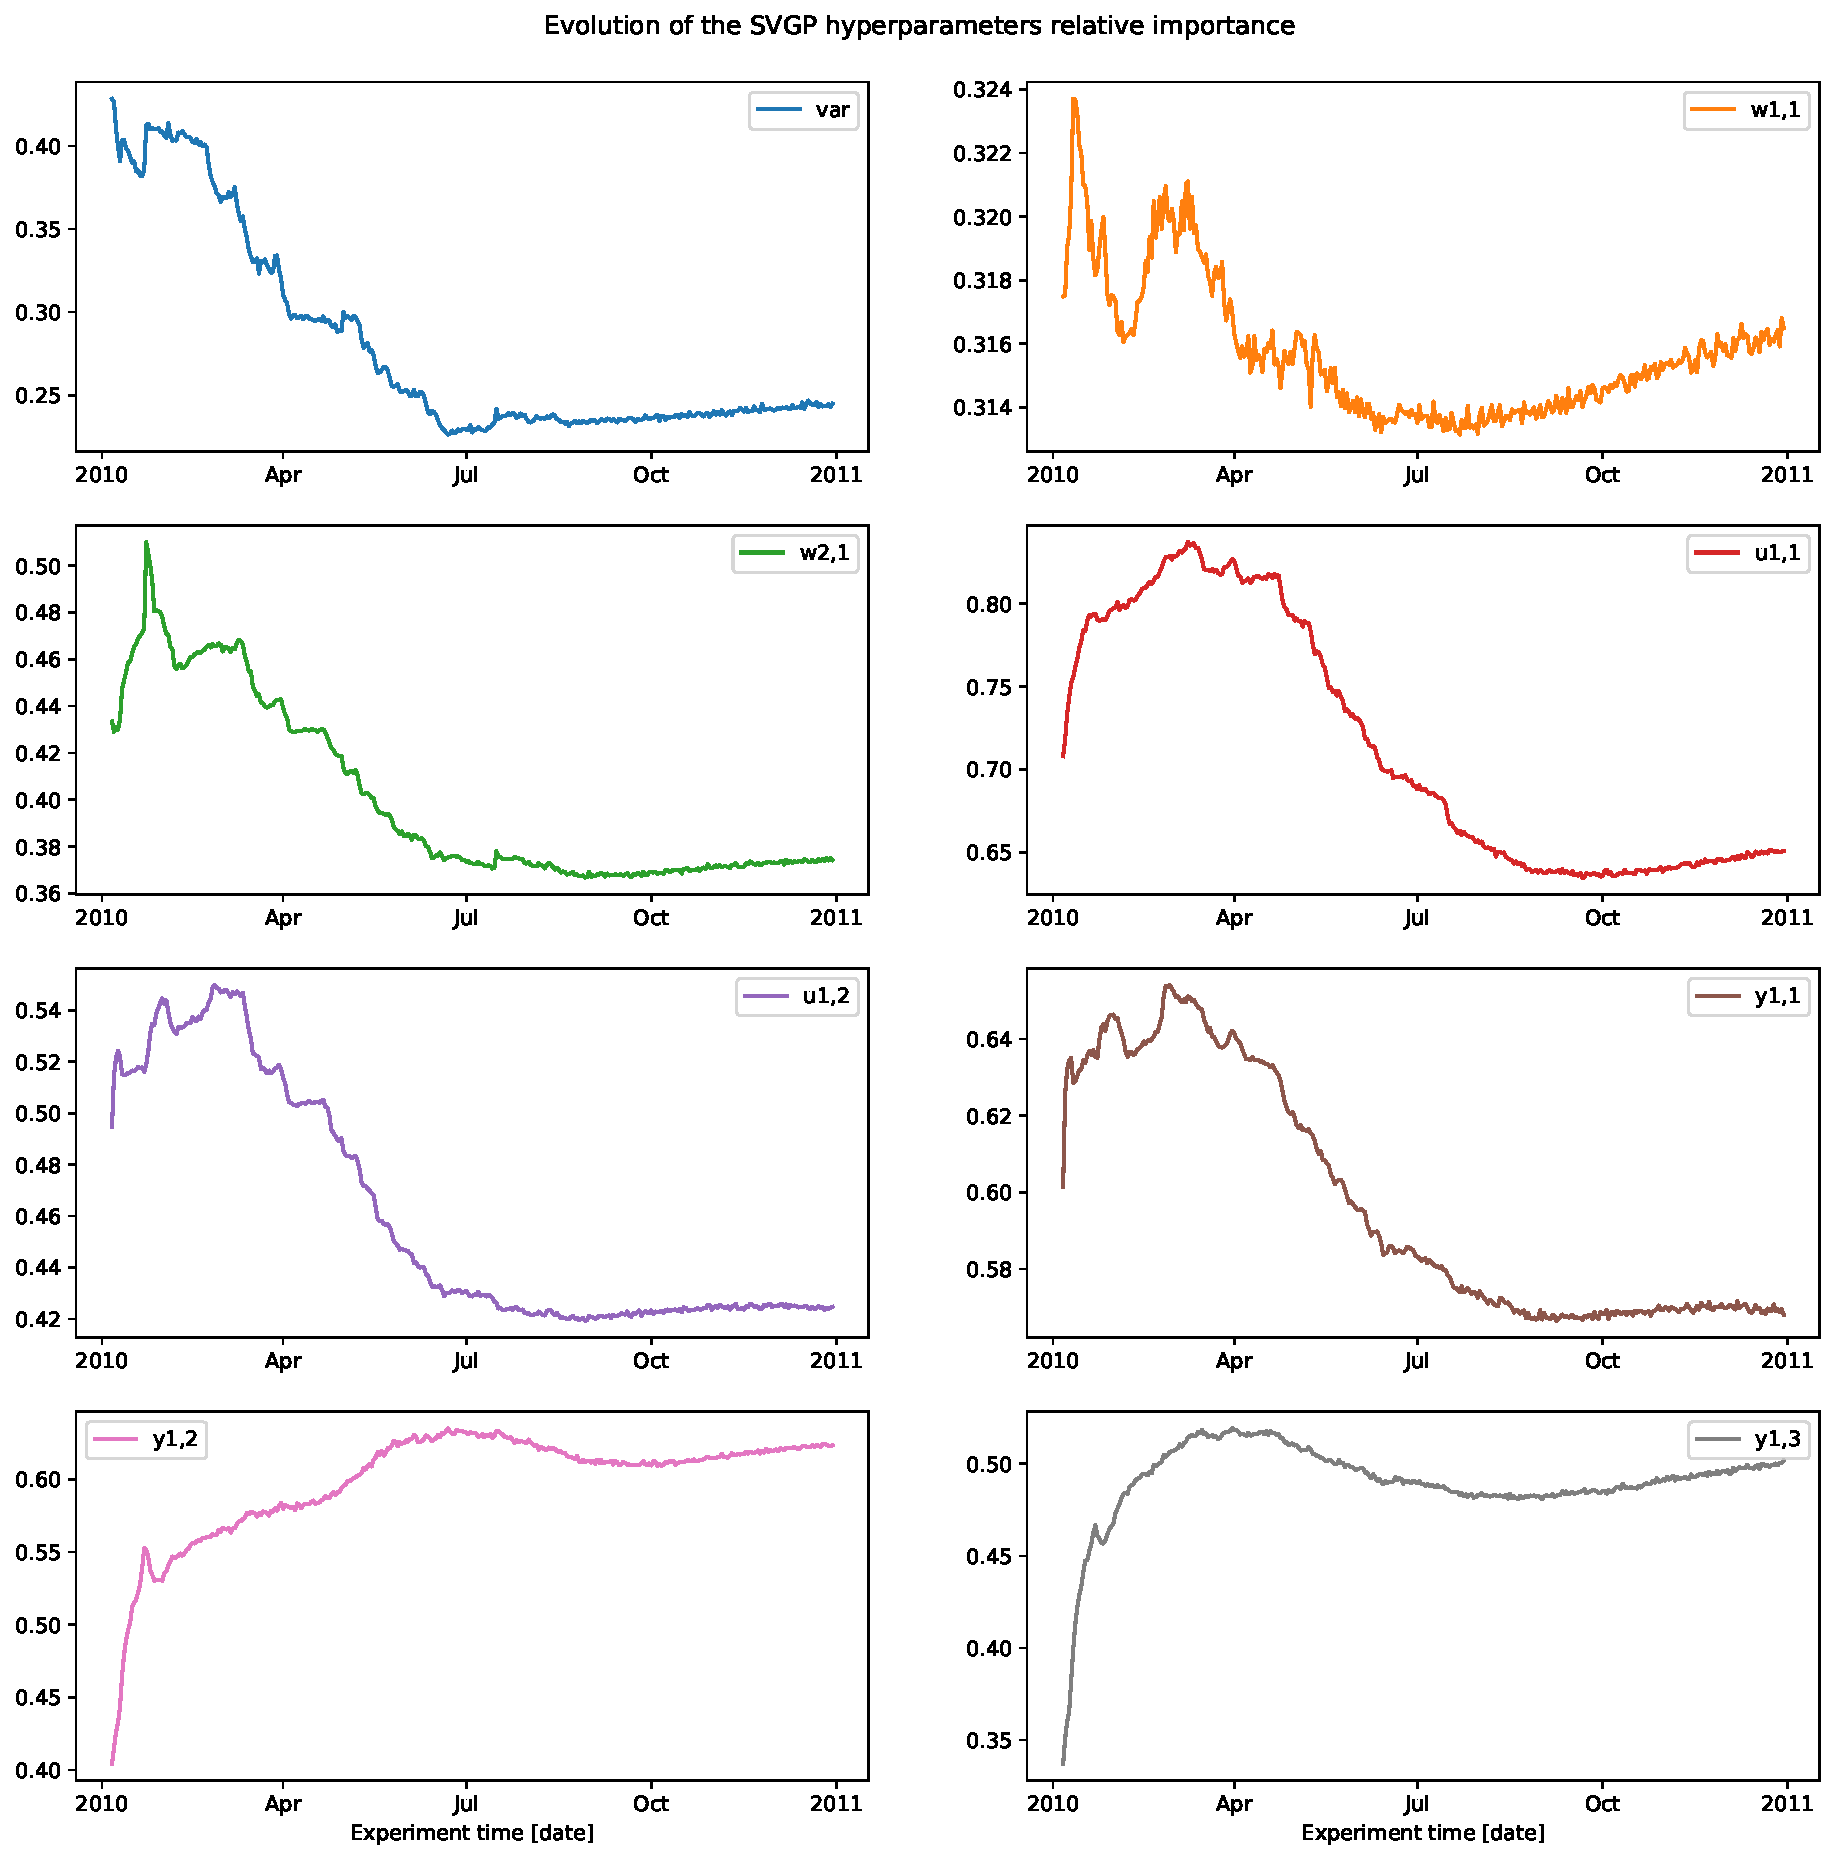
\includegraphics[width =
    \textwidth]{Plots/1_SVGP_480pts_inf_window_12_averageYear_evol_importance.pdf}
    \caption{Evolution of SVGP model parameters}
    \label{fig:SVGP_evol_importance}
\end{figure}

As seen in Figure~\ref{fig:SVGP_evol_importance}, the variance of the
\acrshort{se} kernel steadily decreases, until reaching a plateau, which
signifies the increase in confidence of the model. The hyperparameters
corresponding to the exogenous inputs --- $w1,1$ and $w1,2$ --- become generally
less important for future predictions over the course of the year, with the
importance of $w1,1$, the \acrlong{ghi}, climbing back up over the last, colder
months. This might be due to the fact that during the colder months, the
\acrshort{ghi} is the only way for the exogenous inputs to \textit{provide}
additional heat to the system.

A similar trend can be observed for the evolution of the input's
hyperparameters, with the exception that the first lag of the controlled input,
$u1,1$ remains the most important over the course of the year.

For the lags of the measured output it can be seen that, over the course of the
year, the importance of the first lag decreases, while that of the second and
third lag increase --- until all three reach relatively similar values.

Another interesting comparison is provided by looking at the possible values of
the \acrshort{se} kernel components. Since all the values are normalized within
the -1 to 1 range, it is unlikely that any two points will be a distance higher
than 2 apart. It is possible then to plot the values of the kernel terms due to
each regressor as a function of their distance. This is done in
Figure~\ref{fig:SVGP_first_covariance} for the first identified model and in
Figure~\ref{fig:SVGP_last_covariance} for the last. It is clear that in both
cases the kernel terms behave mostly linearly, with the exception of two points
being close to each other, when the correlation remains stronger before it
starts diminishing.

\begin{figure}[ht]
    \centering
    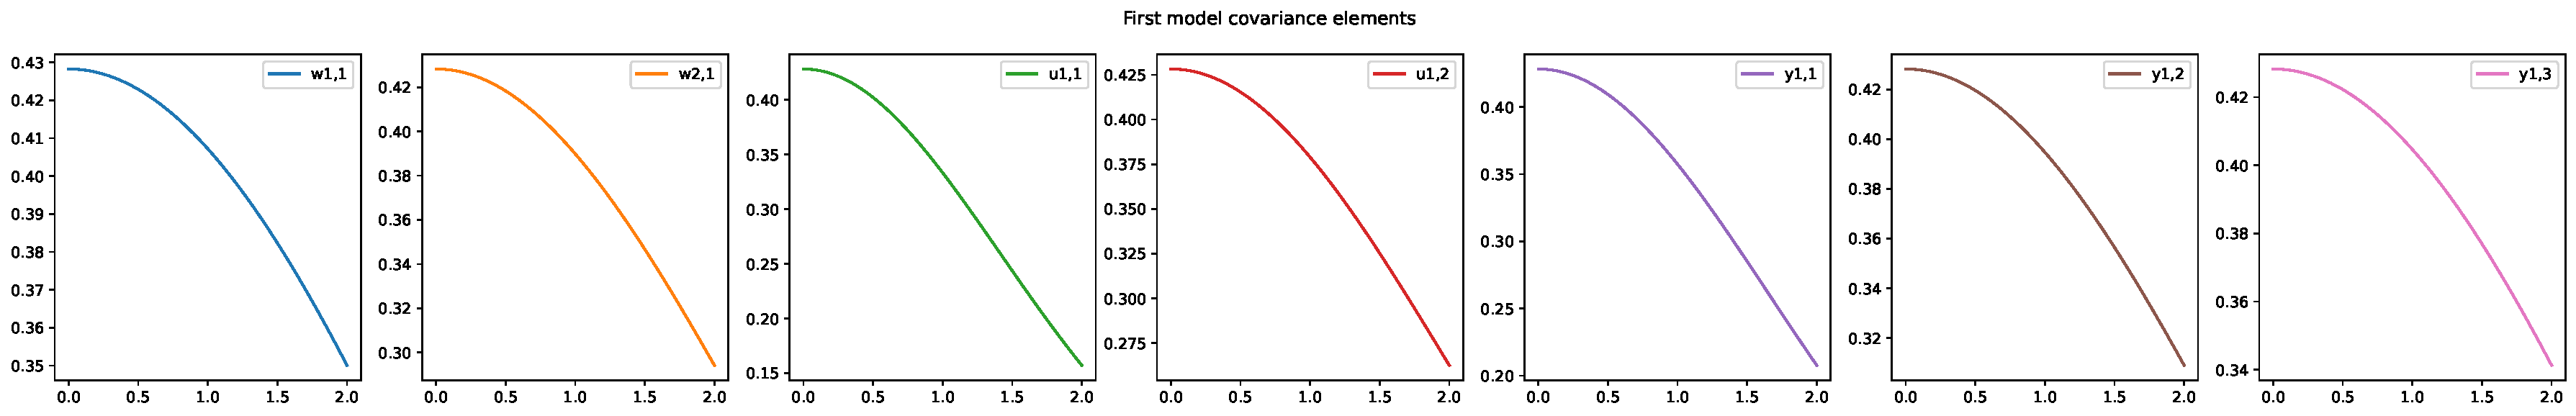
\includegraphics[width =
    \textwidth]{Plots/1_SVGP_480pts_inf_window_12_averageYear_first_covariance.pdf}
    \caption{SVGP model first covariance parameters}
    \label{fig:SVGP_first_covariance}
\end{figure}

As for the last model, it can be noted that only the scale of the kernel terms
changes, with their shape remaining consistent with the first identified model.
This means that the model does not get much more complex as the data is
gathered, but instead the same general structure is kept, with further
refinements being done as data is added to the system.

\begin{figure}[ht]
    \centering
    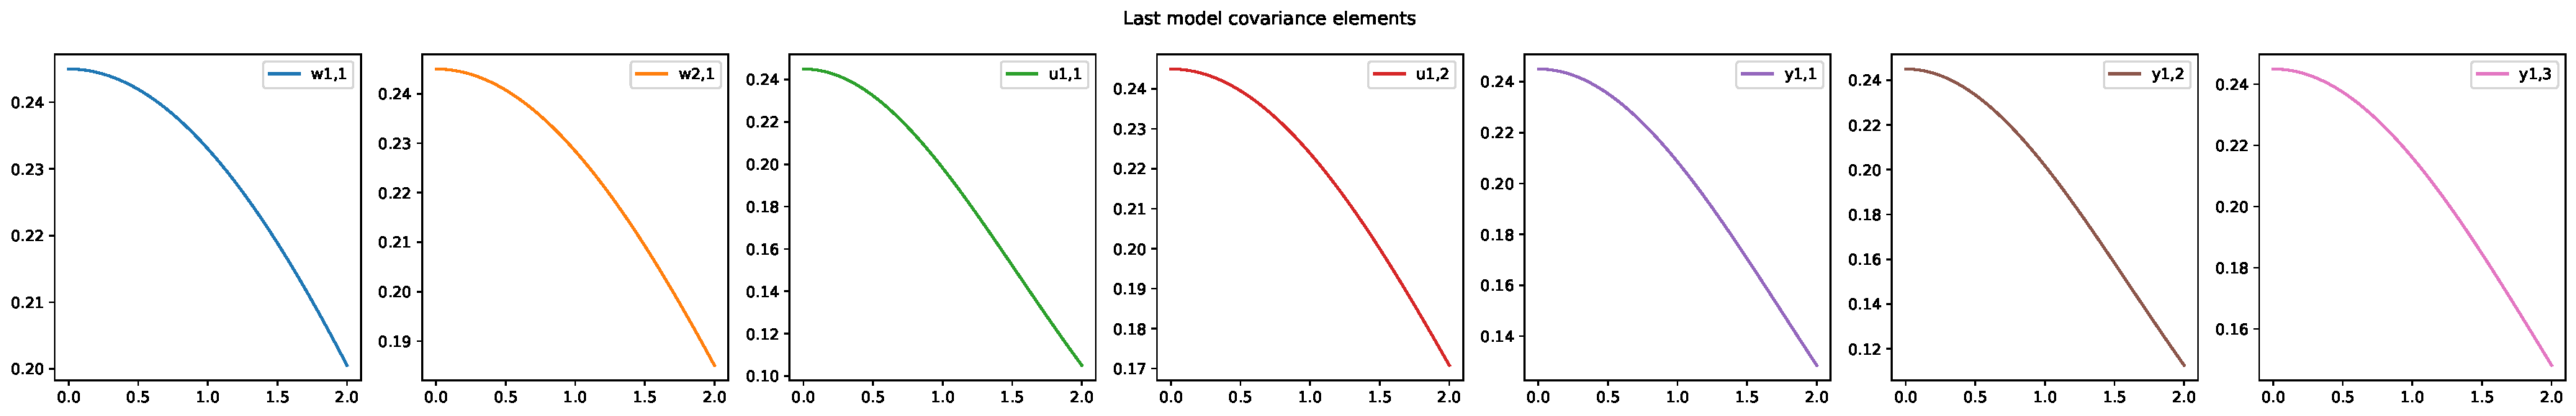
\includegraphics[width =
    \textwidth]{Plots/1_SVGP_480pts_inf_window_12_averageYear_last_covariance.pdf}
    \caption{SVGP model last covariance parameters}
    \label{fig:SVGP_last_covariance}
\end{figure}

One question that could be addressed given these mostly linear kernel terms is
how well would an \acrshort{svgp} model perform with a linear kernel.
Intuition would hint that it should still be able to track the reference
temperature, albeit not as precisely due to the correlation that diminished much
slower when the two points are closer together in the \acrshort{se} kernel. This
will be further investigated in Section~\ref{sec:svgp_linear}.

\clearpage

\subsection{SVGP with one day of starting data}\label{sec:svgp_96pts}

As previously discussed in Section~\ref{sec:SVGP_results}, the \acrshort{svgp}
model is able to properly adapt given new information, overtime refining it's
understanding of the plant's dynamics.

Analyzing the results of a simulation done on only one day's worth of initial
simulation data (cf. Figures~\ref{fig:SVGP_96pts_fullyear_simulation}
and~\ref{fig:SVGP_96pts_abserr}) it is very notable that the model performs
almost identically to the one identified in the previous sections. This
nightlights one of the practical benefits of the \acrshort{svgp} implementations
compared to the classical \acrlong{gp} -- it is possible to start with a more
rough controller trained on less data and refine it over time, reducing the need
for cumbersome and potentially costly initial experiments for gathering data.

\begin{figure}[ht]
    \centering
    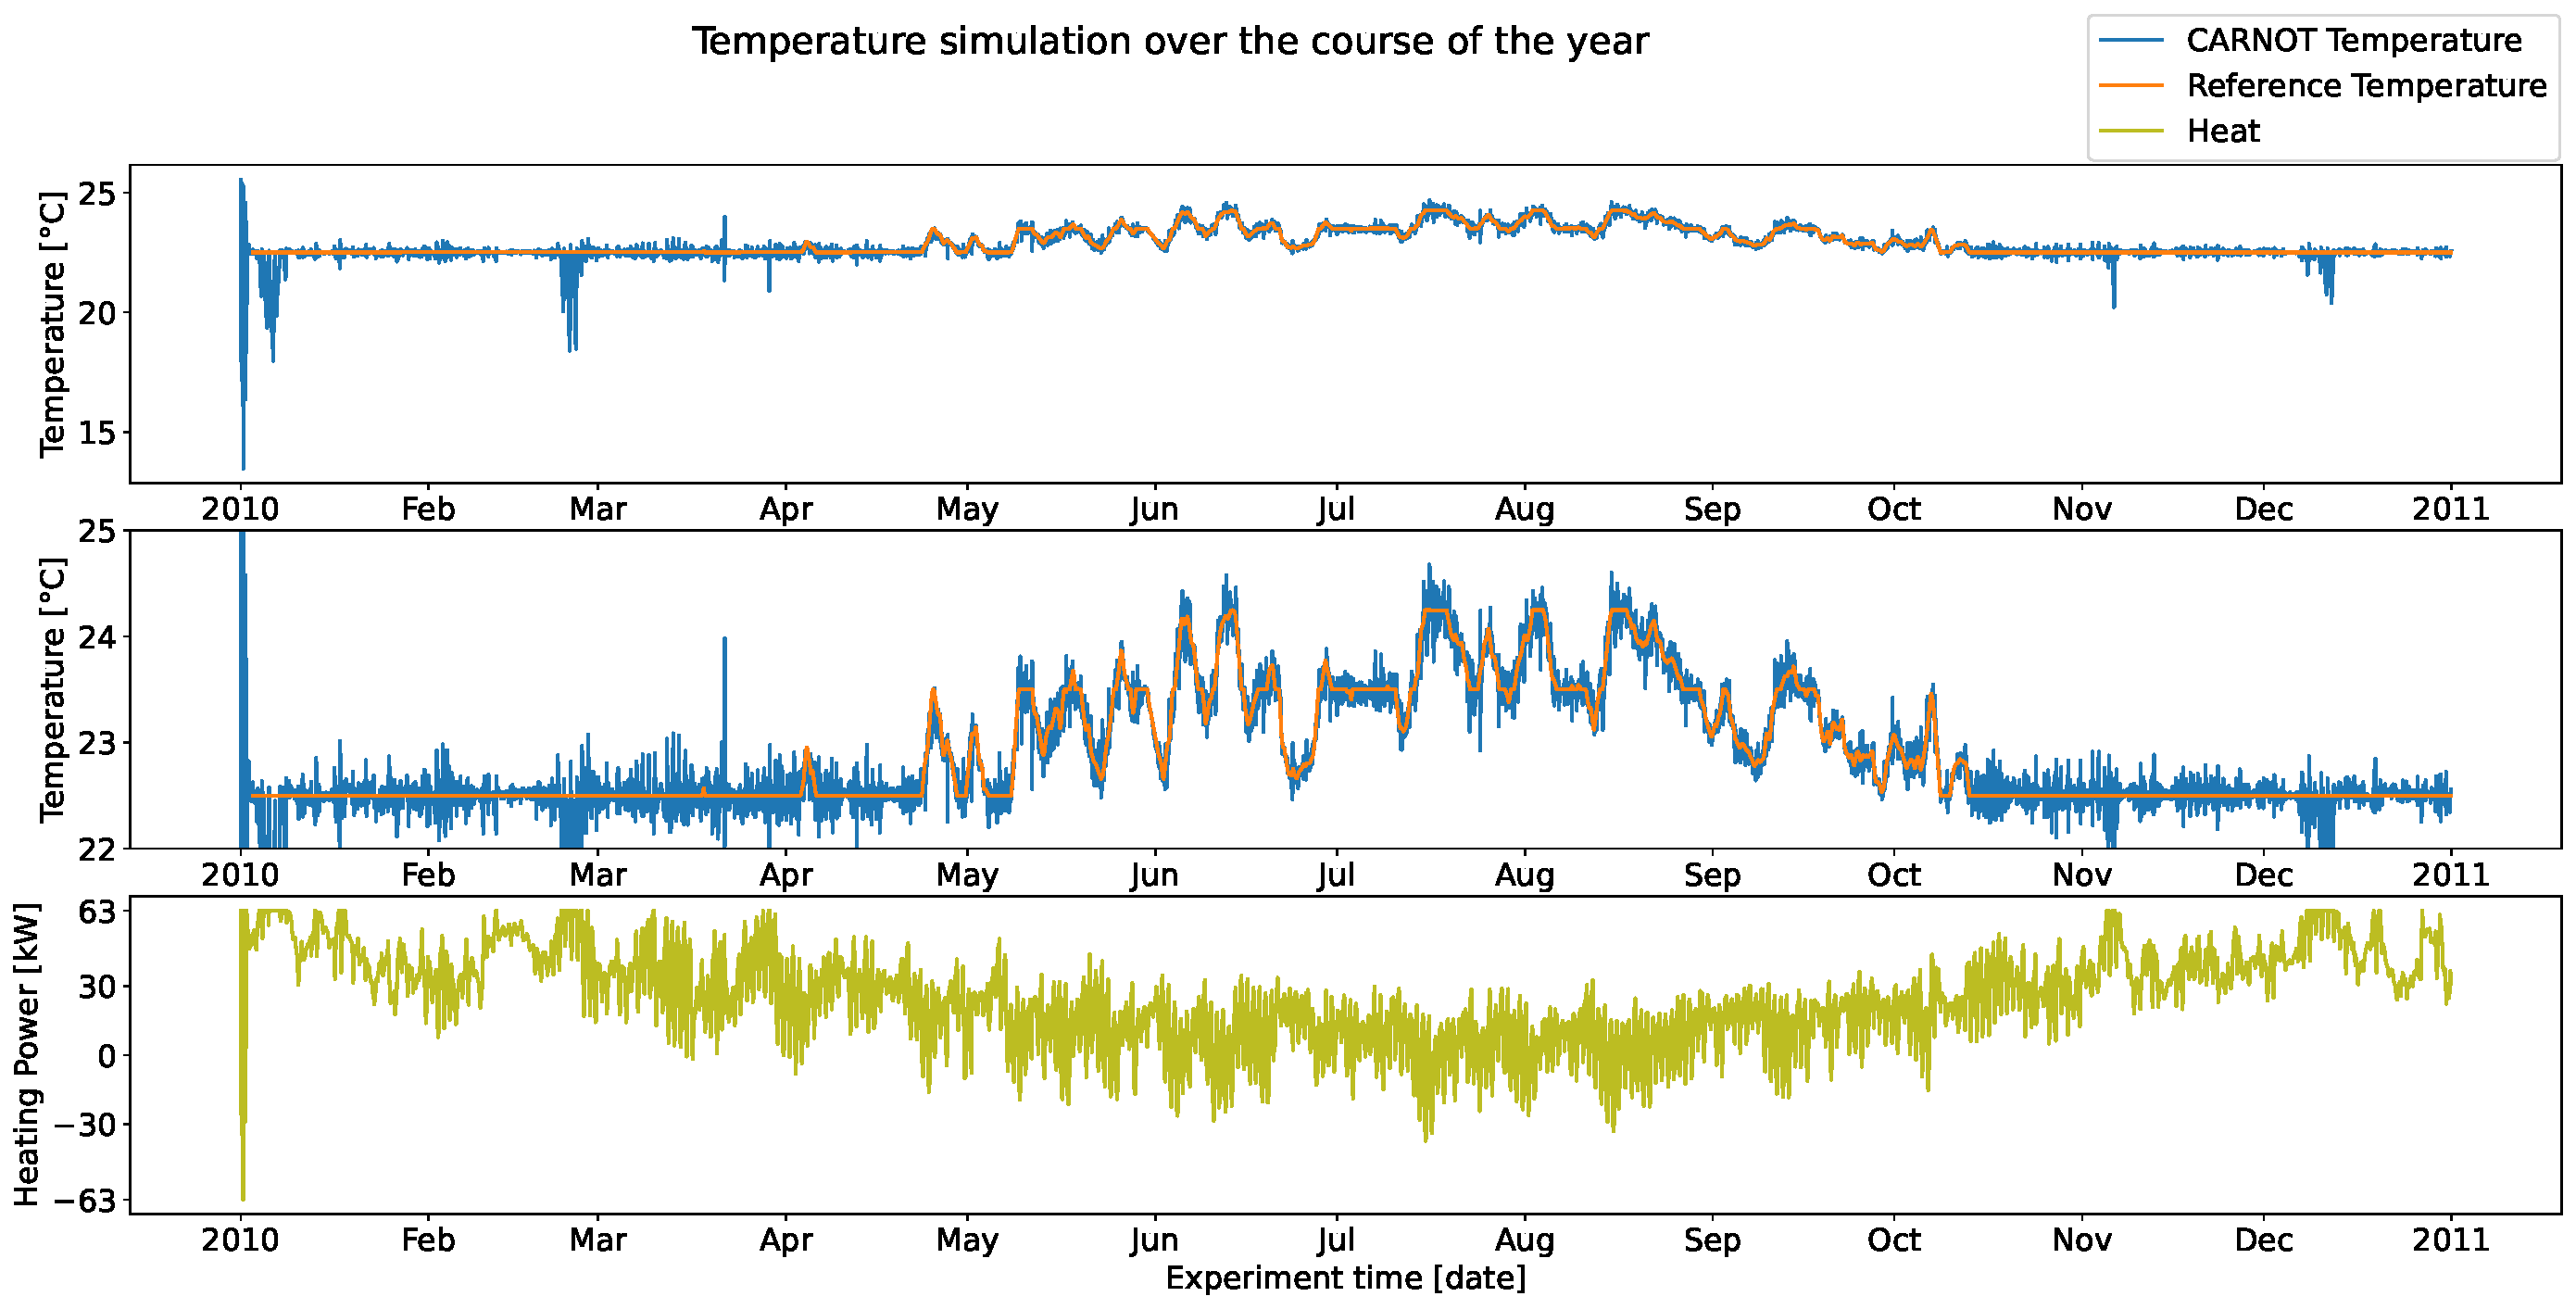
\includegraphics[width =
    \textwidth]{Plots/6_SVGP_96pts_inf_window_12_averageYear_fullyear.pdf}
    \caption{One Day SVGP full year simulation}
    \label{fig:SVGP_96pts_fullyear_simulation}
\end{figure}

\begin{figure}[ht]
    \centering
    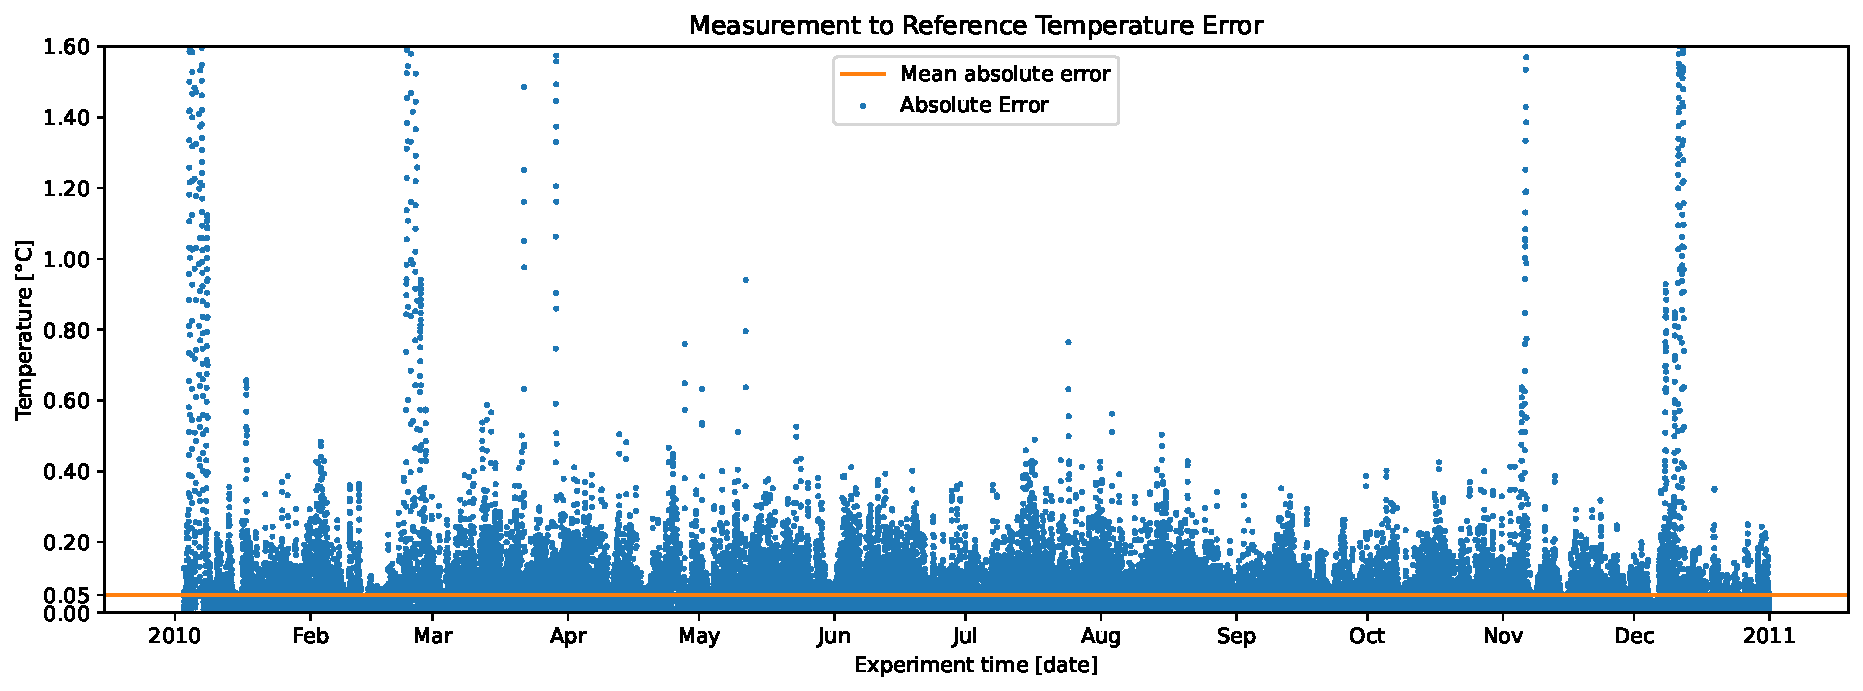
\includegraphics[width =
    \textwidth]{Plots/6_SVGP_96pts_inf_window_12_averageYear_abserr.pdf}
    \caption{One Day SVGP Absolute Error}
    \label{fig:SVGP_96pts_abserr}
\end{figure}

\subsection{SVGP with a five days moving window}\label{sec:svgp_window}

This section presents the result of running a different control scheme. Here,
as the base \acrshort{svgp} model, it is first trained on 5 days worth of data,
with the difference being that each new model is only identified using the last
five days' worth of data. This should provide an insight on whether the
\acrshort{svgp} model is able to understand model dynamics only based on
closed-loop operation.

\begin{figure}[ht]
    \centering
    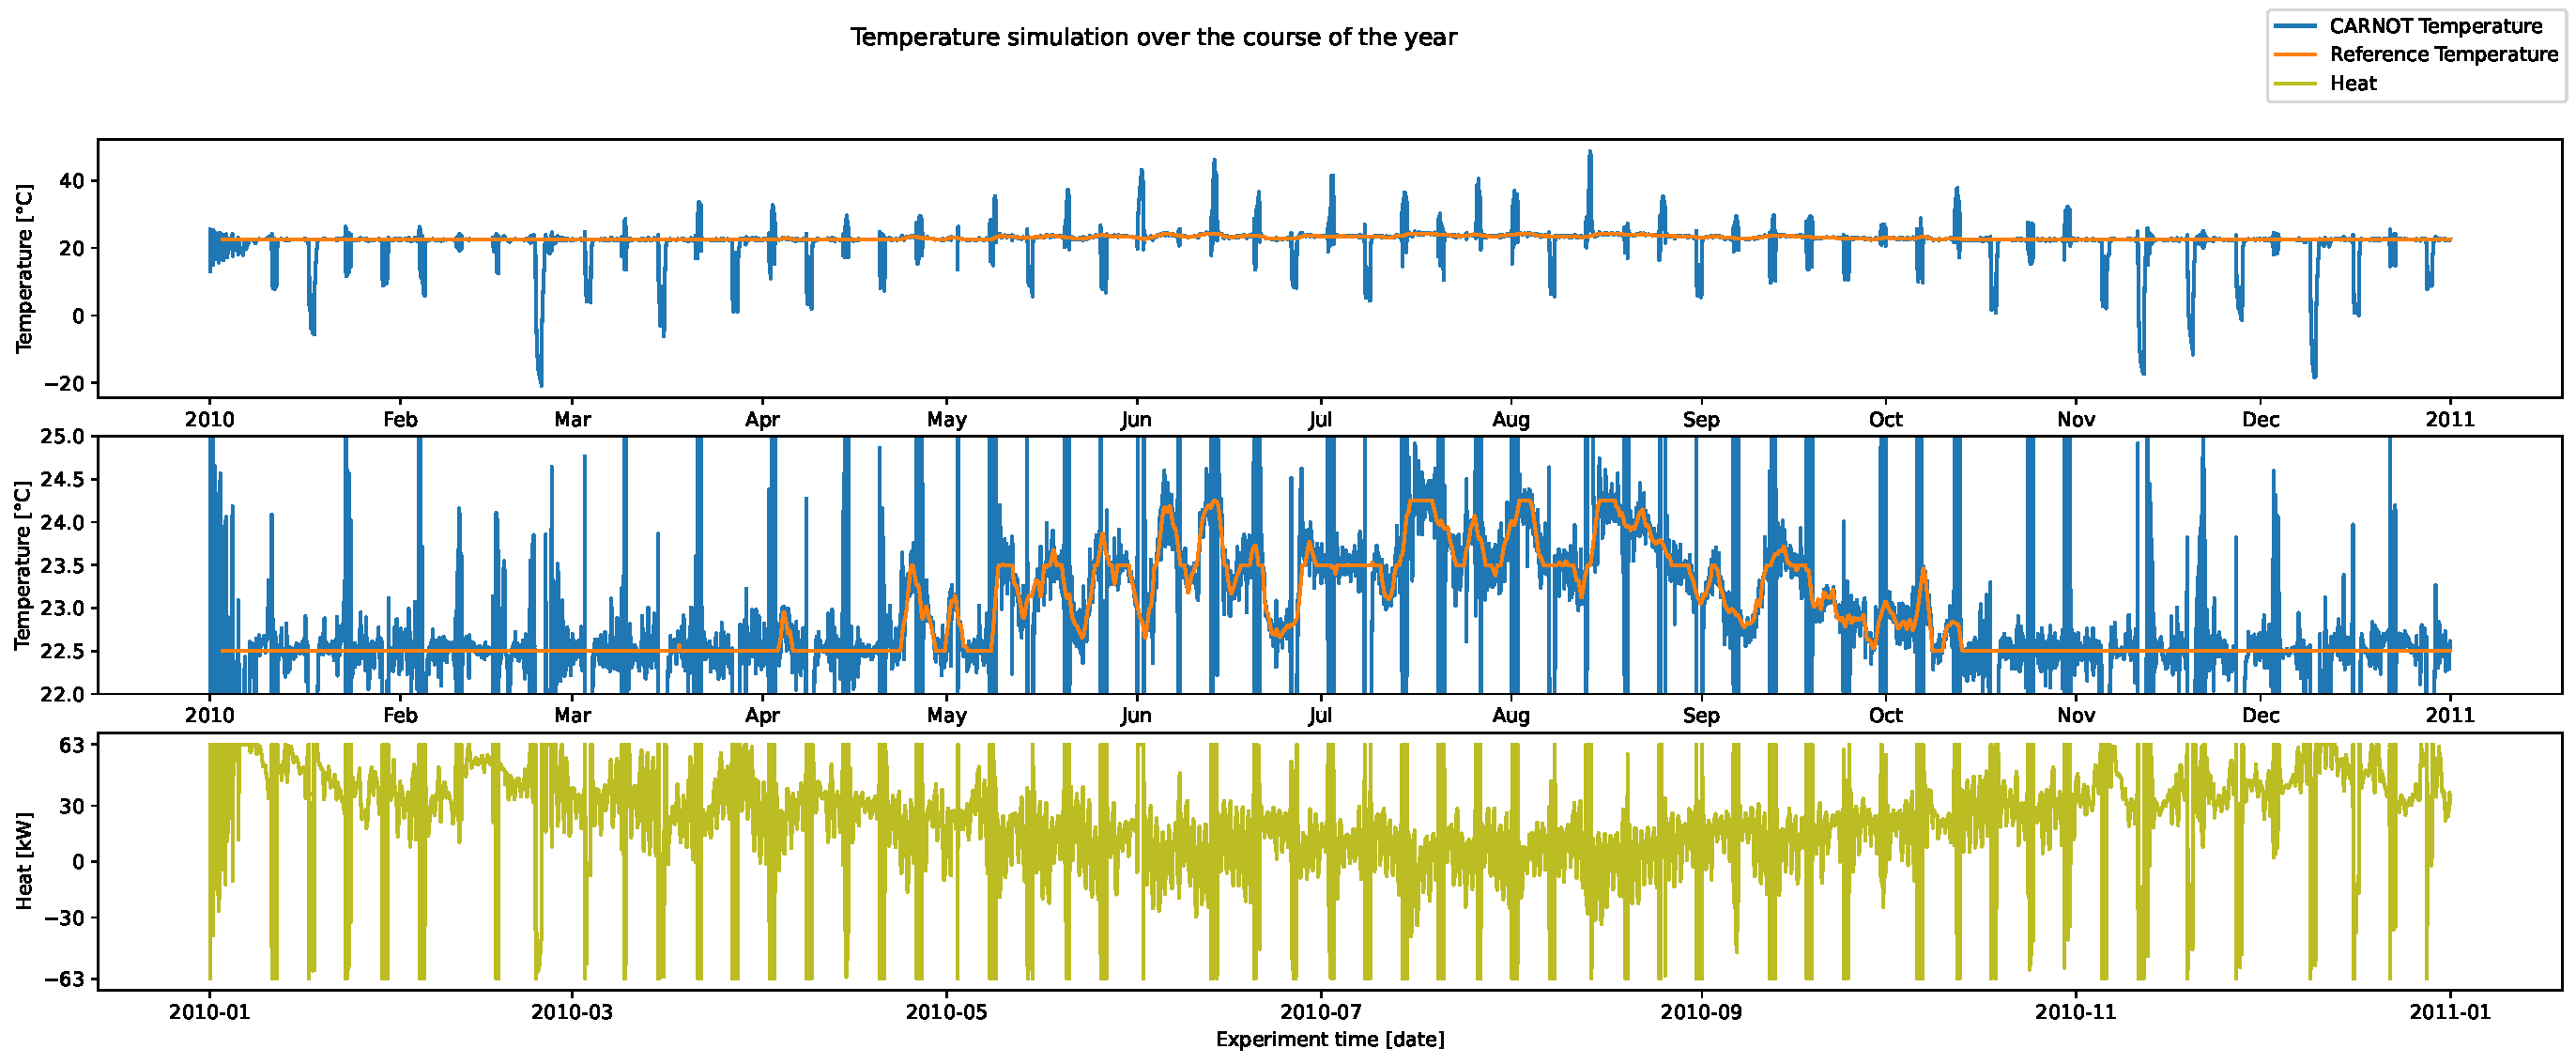
\includegraphics[width =
    \textwidth]{Plots/5_SVGP_480pts_480pts_window_12_averageYear_fullyear.pdf}
    \caption{SVGP full year simulation}
    \label{fig:SVGP_480window_fullyear_simulation}
\end{figure}

As it can be seen in Figure~\ref{fig:SVGP_480window_fullyear_simulation}, this
model is unable to properly track the reference temperature. In fact, five days
after the identification the model forgets all the initial data and becomes
unstable. This instability then generates enough excitation of the plant for the
model to again learn its behaviour. This cycle repeats every five days, when the
controller becomes unstable. In the stable regions, however, the controller is
able to track the reference temperature. 

\subsection{SVGP with Linear Kernel}\label{sec:svgp_linear}

The last model to be investigated is the \acrshort{svgp} with Linear Kernel. As
it was suggested previously, the terms of the originally identified
\acrshort{svgp} model are not very complex, leading to the question whether a
pure linear kernel could suffice to understand the plant's behaviour.

Figure~\ref{fig:SVGP_linear_fullyear_simulation} shows the results of the
full-year simulation. While this controller is still able to track the reference
temperature, it shows a much larger variance in the measured values than the
\acrshort{se} kernel \acrshort{svgp} model. This confirms the previous
suspicions that a pure linear model would not be able to capture the more
nuanced details of the CARNOT model dynamics.

\begin{figure}[ht]
    \centering
    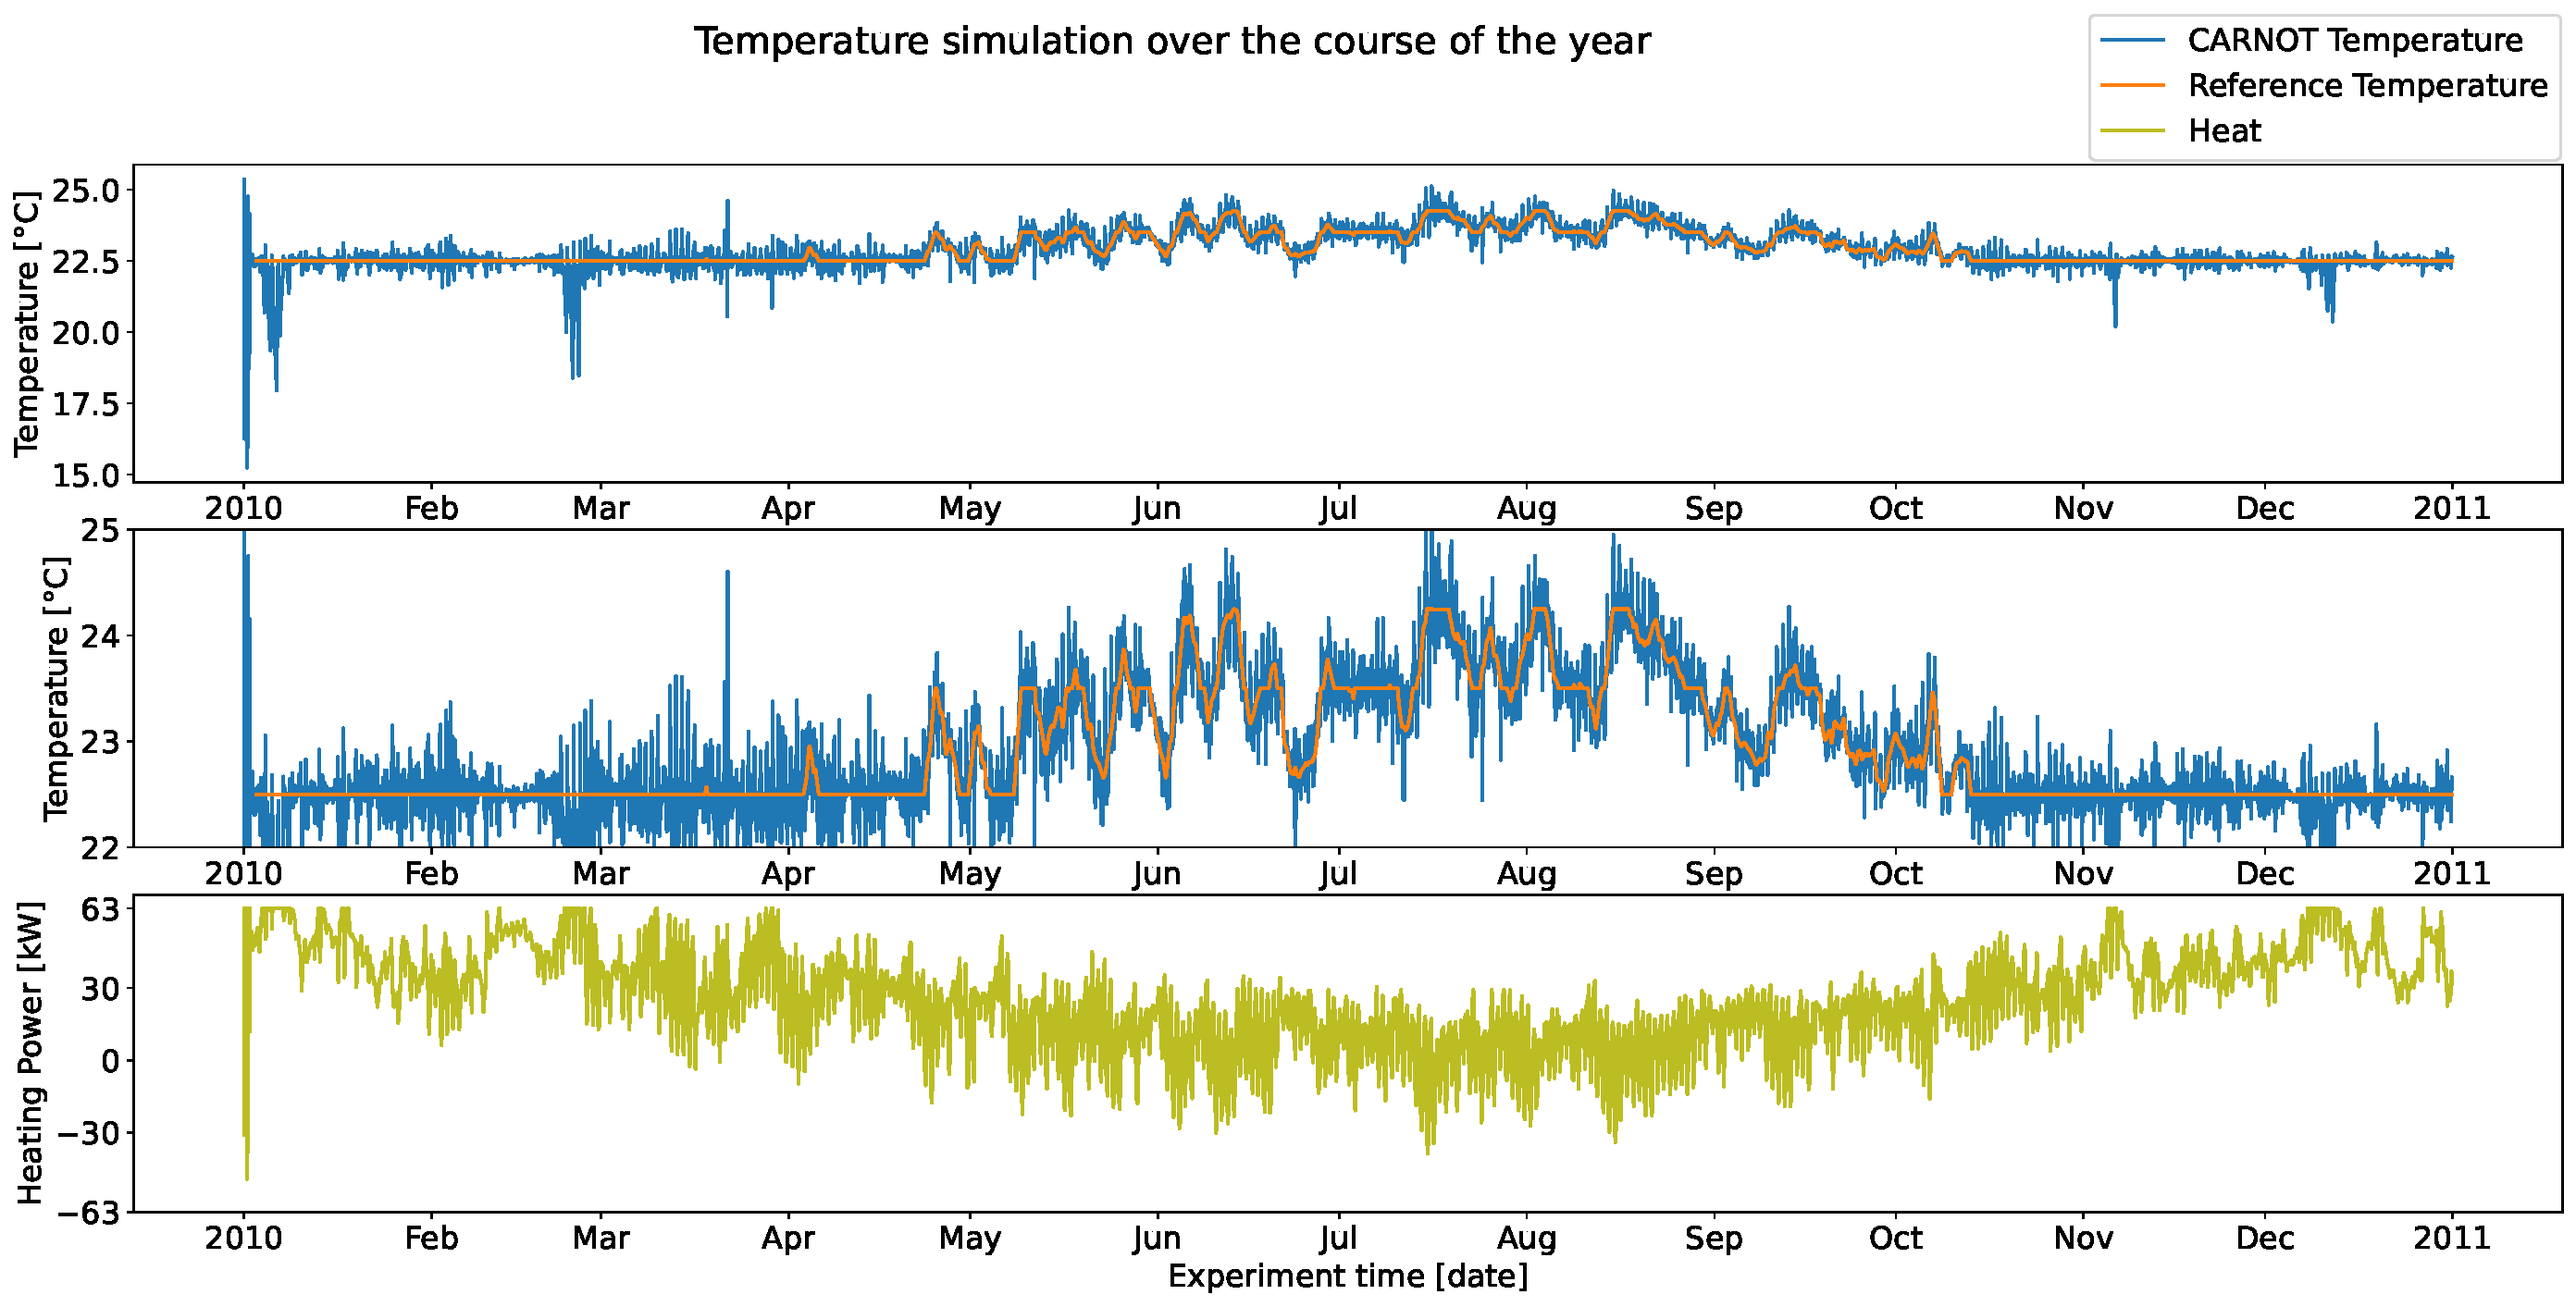
\includegraphics[width =
    \textwidth]{Plots/10_SVGP_480pts_inf_window_12_averageYear_LinearKernel_fullyear.pdf}
    \caption{SVGP full year simulation}
    \label{fig:SVGP_linear_fullyear_simulation}
\end{figure}

\clearpage

\subsection{Comparative analysis}

This section will compare all the results presented in the previous Sections and
try to analyze the differences and their origin.

Presented in Table~\ref{tab:Model_comparations} are the Mean Error, Error
Variance and Mean Absolute Error for the full year simulation for the three
stable \acrshort{svgp} models, as well as the classical \acrshort{gp} model. 

\begin{table}[ht]
%\vspace{-8pt}
\centering
    \begin{tabular}{||c c c c||}
        \hline
        Model & Mean Error [$\degree$C] & Error Variance [$\degree$C] & Mean
        Absolute Error [$\degree$C]\\
        \hline \hline
        GP & 5.08 & 6.88 & 1.330 \\ 
        SVGP (5 days) & -0.06 & 0.25 & 0.055 \\ 
        SVGP (1 day) & -0.04 & 0.24 & 0.050 \\ 
        SVGP (Linear)& -0.03 & 0.29 & 0.093 \\ 
        \hline
    \end{tabular}
\caption{Full-year model performance comparison}
\label{tab:Model_comparations}
\end{table}

The worst performing model, as noted previously, is the \acrshort{gp} model. The
\acrshort{svgp} with Linear Kernel results in a stable model with a mean error
very close to zero, which means no constant bias/ offset. This model has the
highest error variance of all the identified \acrshort{svgp} models, which was
also noted beforehand from qualitative observations. It is therefore possible to
conclude that a Linear Kernel does not suffice for properly modeling the
dynamics of the CARNOT model.

The two \acrshort{svgp} models with \acrlong{se} kernels perform the best. They
have a comparable performance, with very small differences in Mean Absolute
Error and Error variance. This leads to the conclusion that the \acrshort{svgp}
models can be deployed with less explicit identification data, but they will
continue to improve over the course of the year as the building passes through
different regions of the state space and more data is collected.

These results do not, however, discredit the use of \acrlong{gp} for use in a
multi-seasonal situation. As shown before, given the same amount of data and
ignoring the computational cost, they perform better than the alternative
\acrshort{svgp} models. The bad initial performance could be mitigated by
sampling the identification data at different points in time during multiple
experiments, updating a fixed-size dataset based on the gained information, as
well as more cleverly designing the kernel to include prior information.


\clearpage

\section{Conclusion}~\label{sec:conclusion}

The aim of this project was to analyze the performance of \acrshort{gp} based
controllers for use in longer lasting implementations, where differences in
building behaviour become important compared to the initially available data.

First, the performance of a classical \acrshort{gp} model trained on five days
worth of experimental data was analyzed. Initially, this model performed very
well both in one step ahead prediction and multi-step ahead simulation over new,
unseen, data. With the change in weather, however, the model shifted from
operating in the interpolated regions to the extrapolated regions of the initial
weather data. In this scenario the model was unable to properly predict the
\pdome\ behaviour and, as a consequence, the \acrshort{mpc} controller became
unstable.

Following that, several \acrshort{svgp} implementations were analyzed. The
initial behaviour exhibited during parameter identification (cf.
Section~\ref{sec:hyperparameters}) showed that the \acrshort{svgp} model was
less capable of capturing building dynamics only based on the initial
experimental dataset, possibly due to the \acrshort{elbo} approximation of the
true log likelihood. While the \acrshort{svgp} model remained stable over the
course of the 20-step ahead simulation, in the later steps it drifted much
further from the real values than the equivalent \acrshort{gp} model.
However, during the full-year simulation, this downside of the \acrshort{svgp}
model was compensated by adding new data to the model training dataset each
night at midnight. The model performance continuously improved over the course
of the simulation, providing much better results overall.

To better analyze the learning behaviour of the \acrshort{svgp} models, three
variations of the initial \acrshort{svgp} were also simulated. The first
variation consisted of training the initial model on only one day's worth of
experimental data, as opposed to five days in the first case. This model was
then regularly updated every night at midnight, just as the initial case. It
turned out to provide very comparable results to the initial model, leading to
the conclusion that the \acrshort{svgp} model can be initially deployed using
much less training data, and it will still be able to correctly capture the
building dynamics on subsequent updates.

The second variation of the \acrshort{svgp} model was re-trained using a rolling
window of five days' worth of data, in order to see the model's ability to learn 
the proper building dynamics based only on closed-loop operation data. This
model turned out to be unstable, and the full-year simulation showed that every
time the model was trained using \textit{only} closed-loop operation data it
turned unstable. This prompted a much higher excitation of the building for the
following day, which in turn provided enough information to train a good model,
that would last until this information was too old to be included in the
training window, at which point the model would turn unstable again.

In the last variation, the \acrshort{svgp} model was trained using a linear
kernel. This model turned out to perform worse overall than the \acrshort{se}
kernel model since it was unable to capture the more nuanced, non-linear
behaviour of the building.


\subsection{Further Research}~\label{sec:further_research}

Section~\ref{sec:results} has presented and compared the results of a full-year
simulation for a classical \acrshort{gp} model, as well as a few incarnations of
\acrshort{svgp} models. The results show that the \acrshort{svgp} have much
better performance, mainly due to the possibility of updating the model
throughout the year. The \acrshort{svgp} models also present a computational
cost advantage both in training and in evaluation, due to several approximations
shown in Section~\ref{sec:gaussian_processes}.

Focusing on the \acrshort{gp} models, there could be several ways of improving
its performance, as noted previously: a more varied identification dataset and
smart update of a fixed-size data dictionary according to information gain,
could mitigate the present problems.

Using a Sparse \acrshort{gp} without replacing the maximum log likelihood
with the \acrshort{elbo} could improve performance of the \acrshort{gp} model at
the expense of training time.

An additional change that could be made is inclusion of the most amount of prior
information possible through setting a more refined kernel, as well as adding
prior information on all the model hyperparameters when available. This approach
however goes against the `spirit' of black-box approaches, since significant
insight into the physics of the plant is required in order to properly model and
implement this information.

On the \acrshort{svgp} side, several changes could also be proposed, which were
not properly addressed in this work. First, the size of the inducing dataset was
chosen experimentally until it was found to accurately reproduce the manually
collected experimental data. In order to better use the available computational
resources, this value could be found programmatically in a way to minimize
evaluation time, while still providing good performance. Another possibility is
the periodic re-evaluation of this value when new data comes in, since as more
and more data is collected the model becomes more complex, and in general more
inducing locations could be necessary to properly reproduce the training data.

Finally, none of the presented controllers take into account occupancy rates or
adapt to possible changes in the real building, such as adding or removing
furniture, deteriorating insulation and so on. The presented update methods only
deals with adding information on behaviour in different state space regions, i.e
\textit{learning}. Additionally, their ability to \textit{adapt} to changes in
the actual plant's behaviour should be further addressed.

\section*{Acknowledgements}

I would like to thank Manuel Koch for the great help provided during the course
of the project starting from the basics on CARNOT modelling, to helping me
better compare the performance of different controllers, as well as Prof.\ Colin
Jones, whose insights were always very guiding, while still allowing me to
discover everything on my own.

\clearpage

\printbibliography[heading=bibintoc]
\appendix
\clearpage

\section{Hyperparameters validation for classical GP}

\subsection{113}

\begin{figure}[ht]
    \centering
    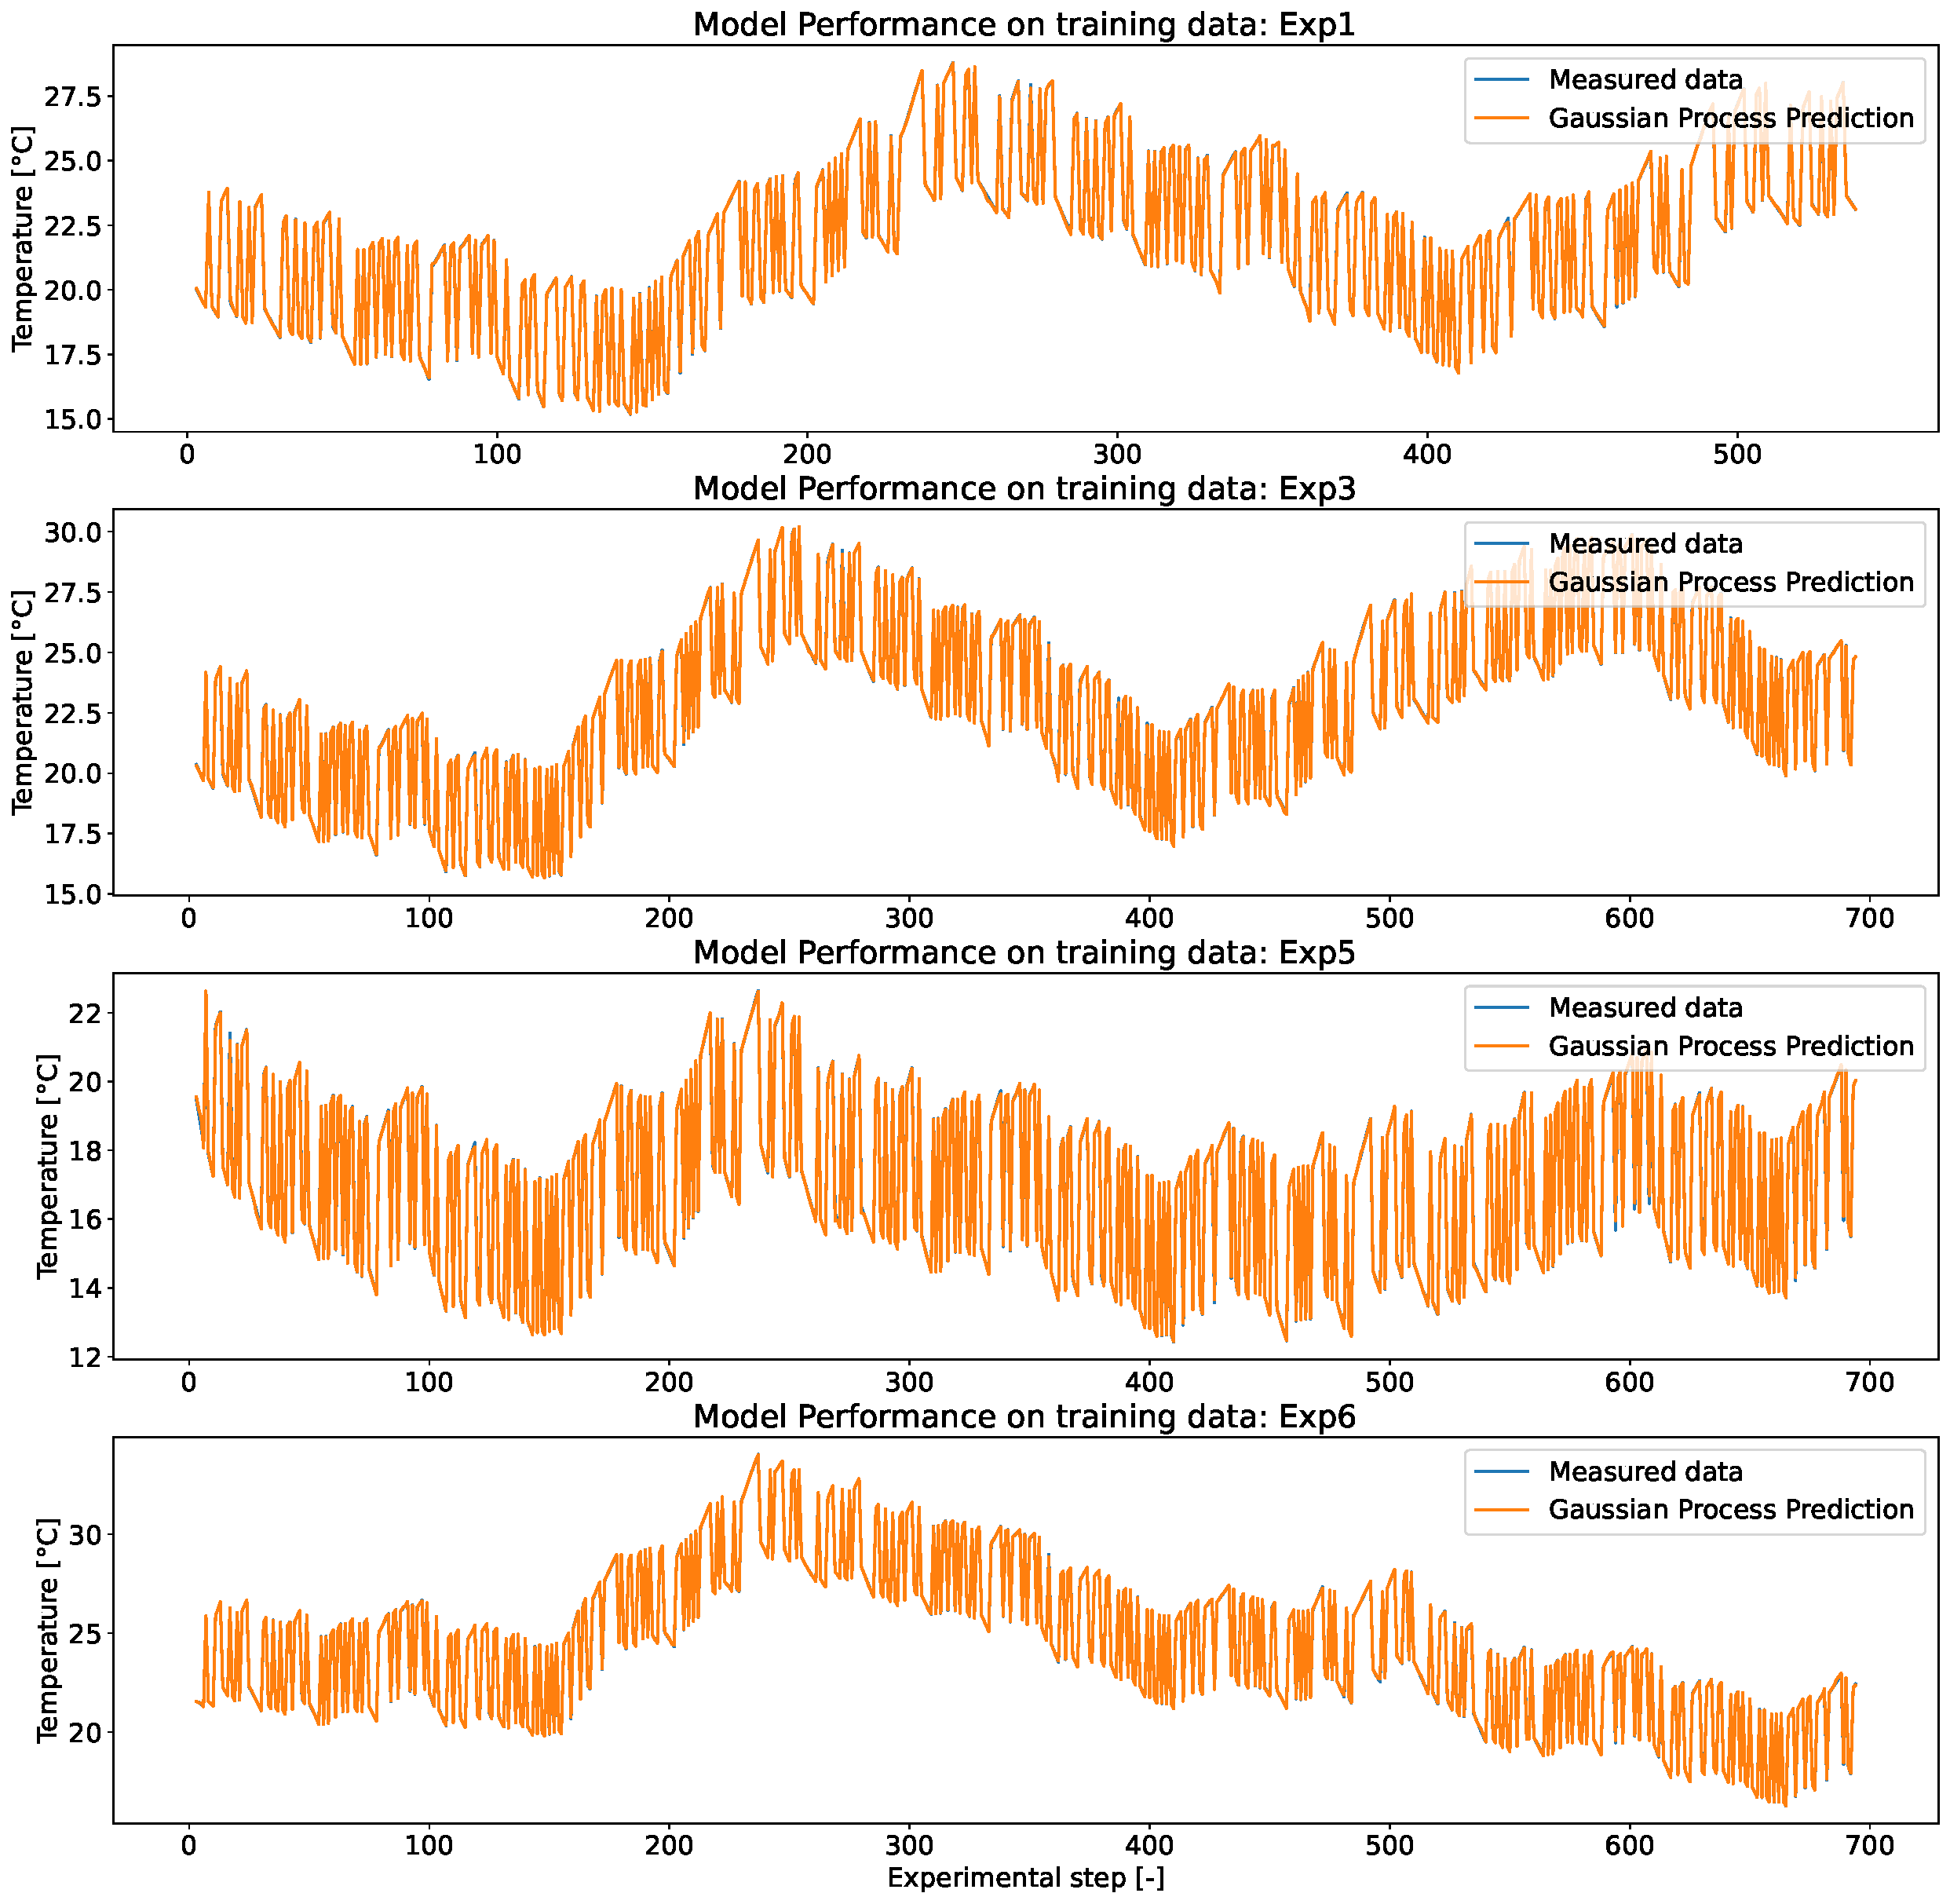
\includegraphics[width = \textwidth]{Plots/GP_113_training_performance.pdf}
    \caption{}
    \label{fig:GP_train_validation}
\end{figure}

\begin{figure}[ht]
    \centering
    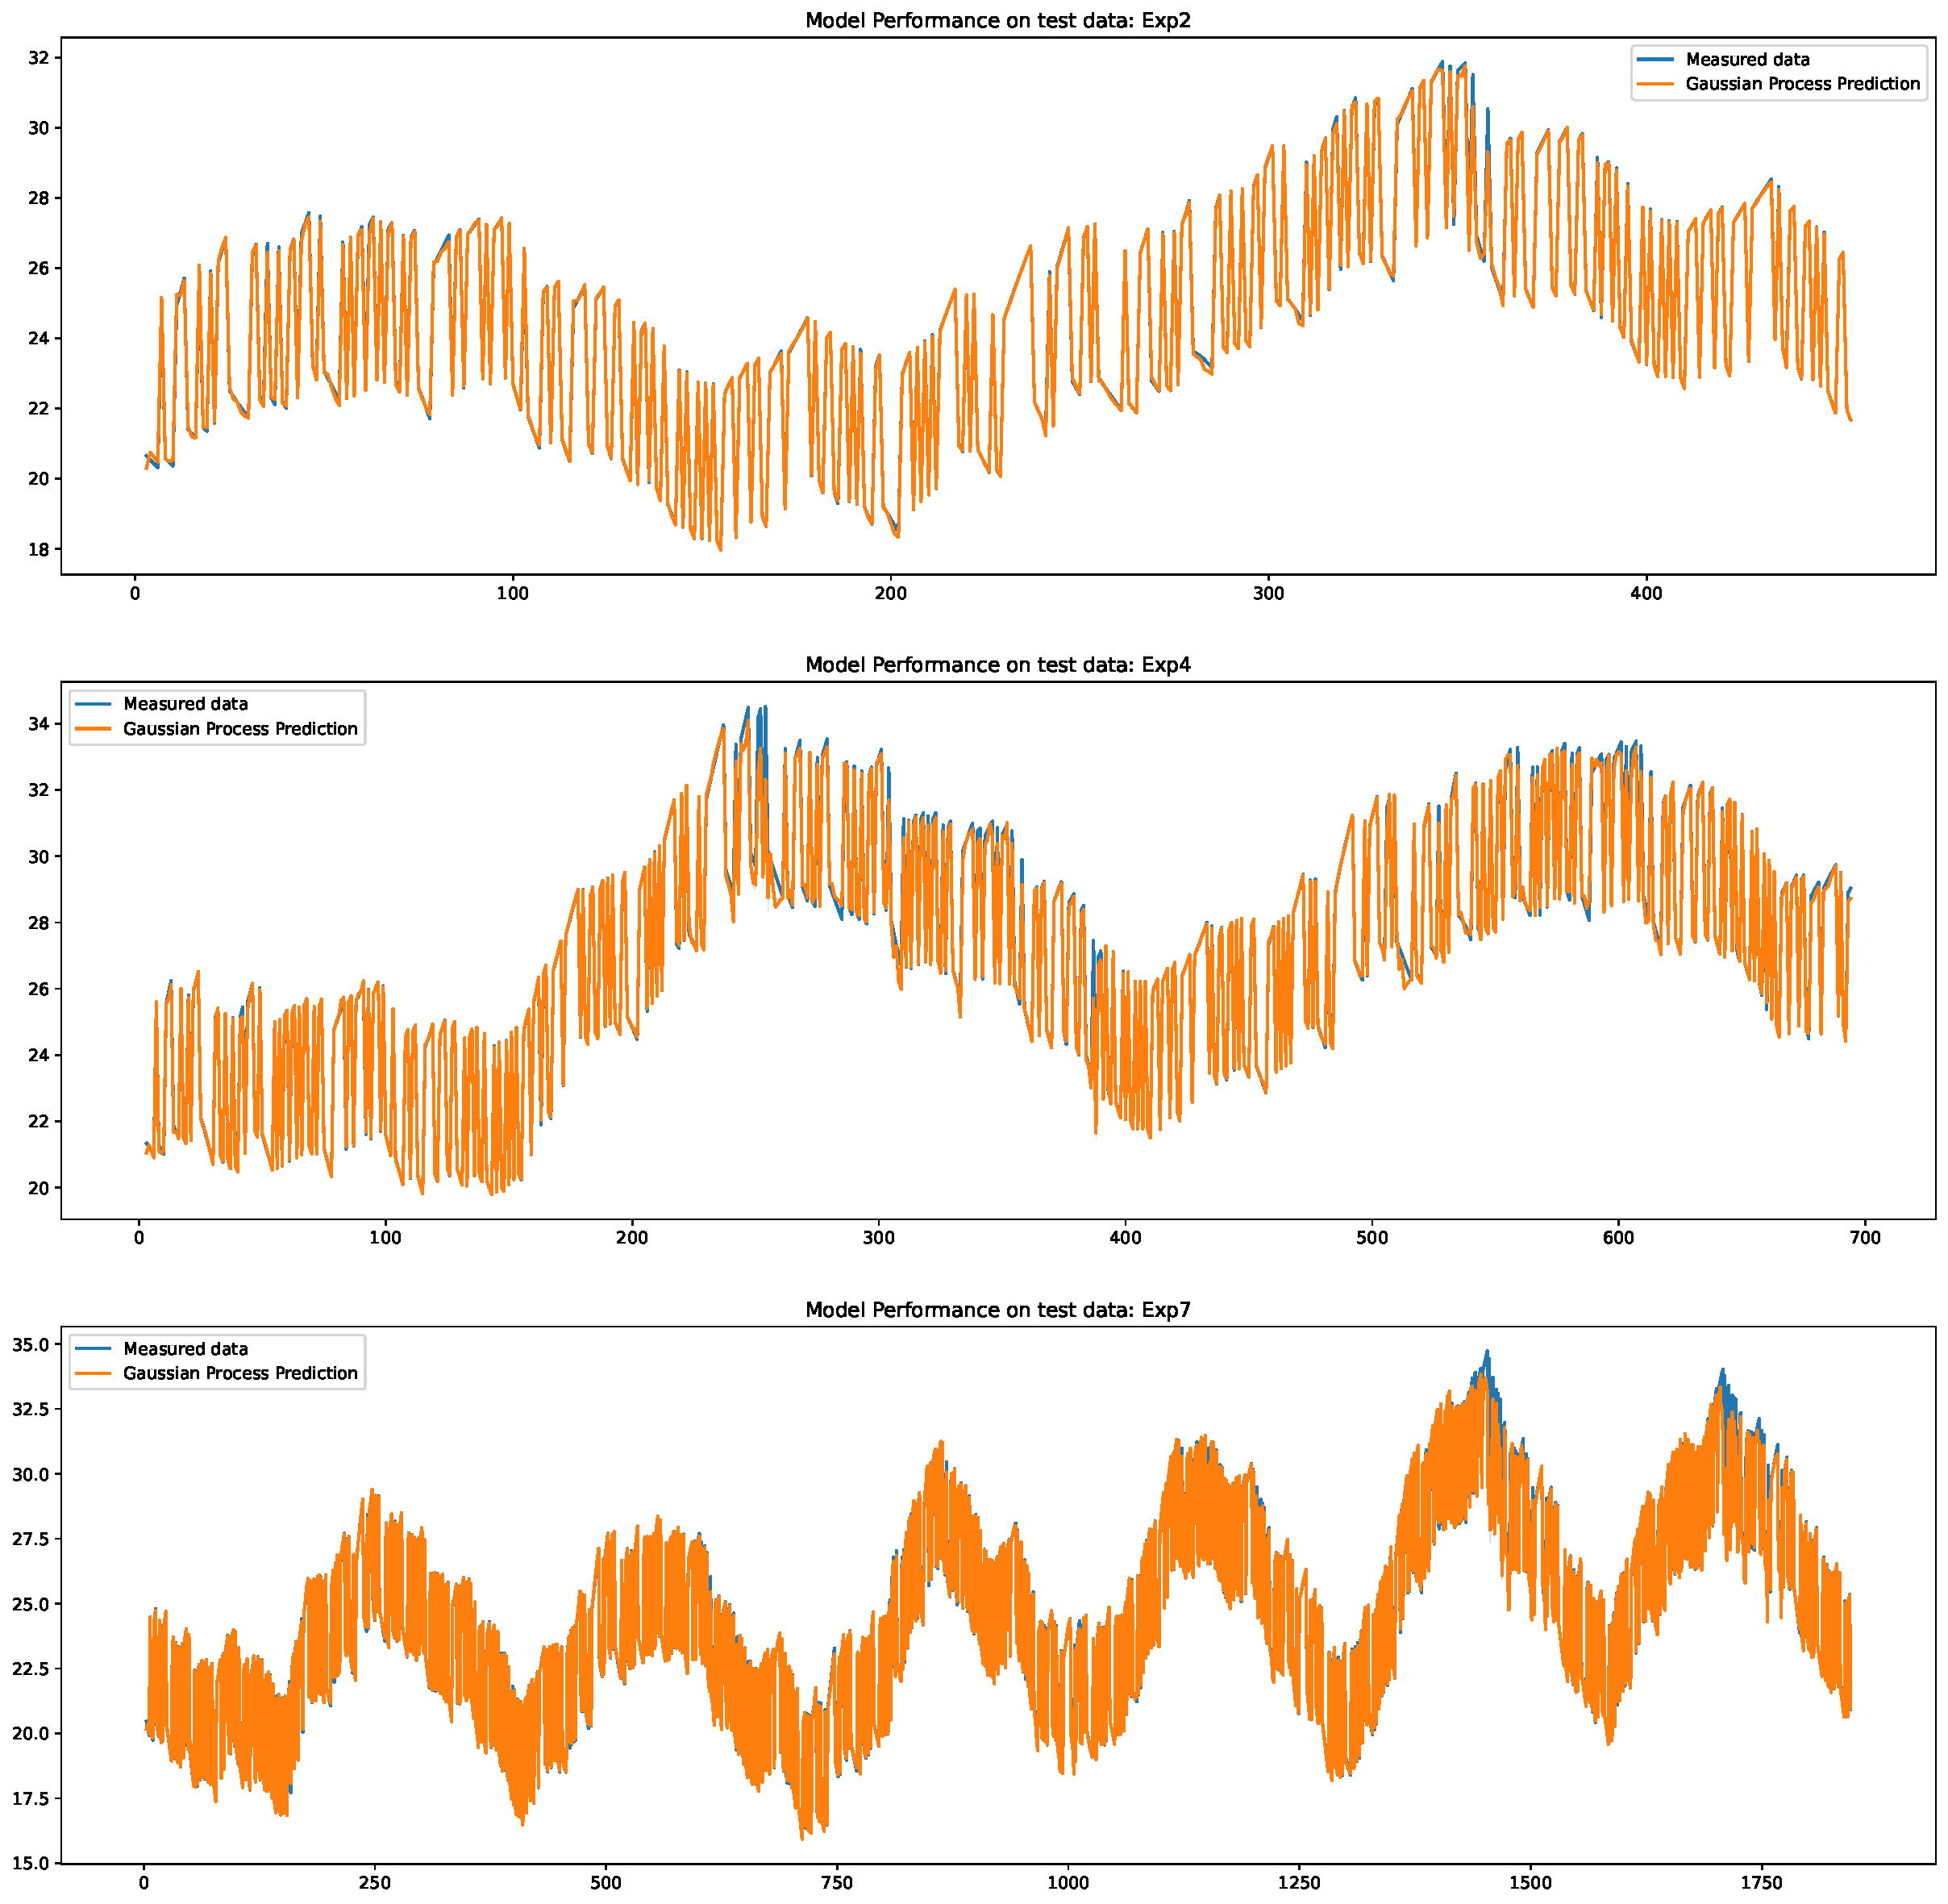
\includegraphics[width = \textwidth]{Plots/GP_113_test_performance.pdf}
    \caption{}
    \label{fig:GP_test_validation}
\end{figure}

\clearpage

\subsection{213}

\begin{figure}[ht]
    \centering
    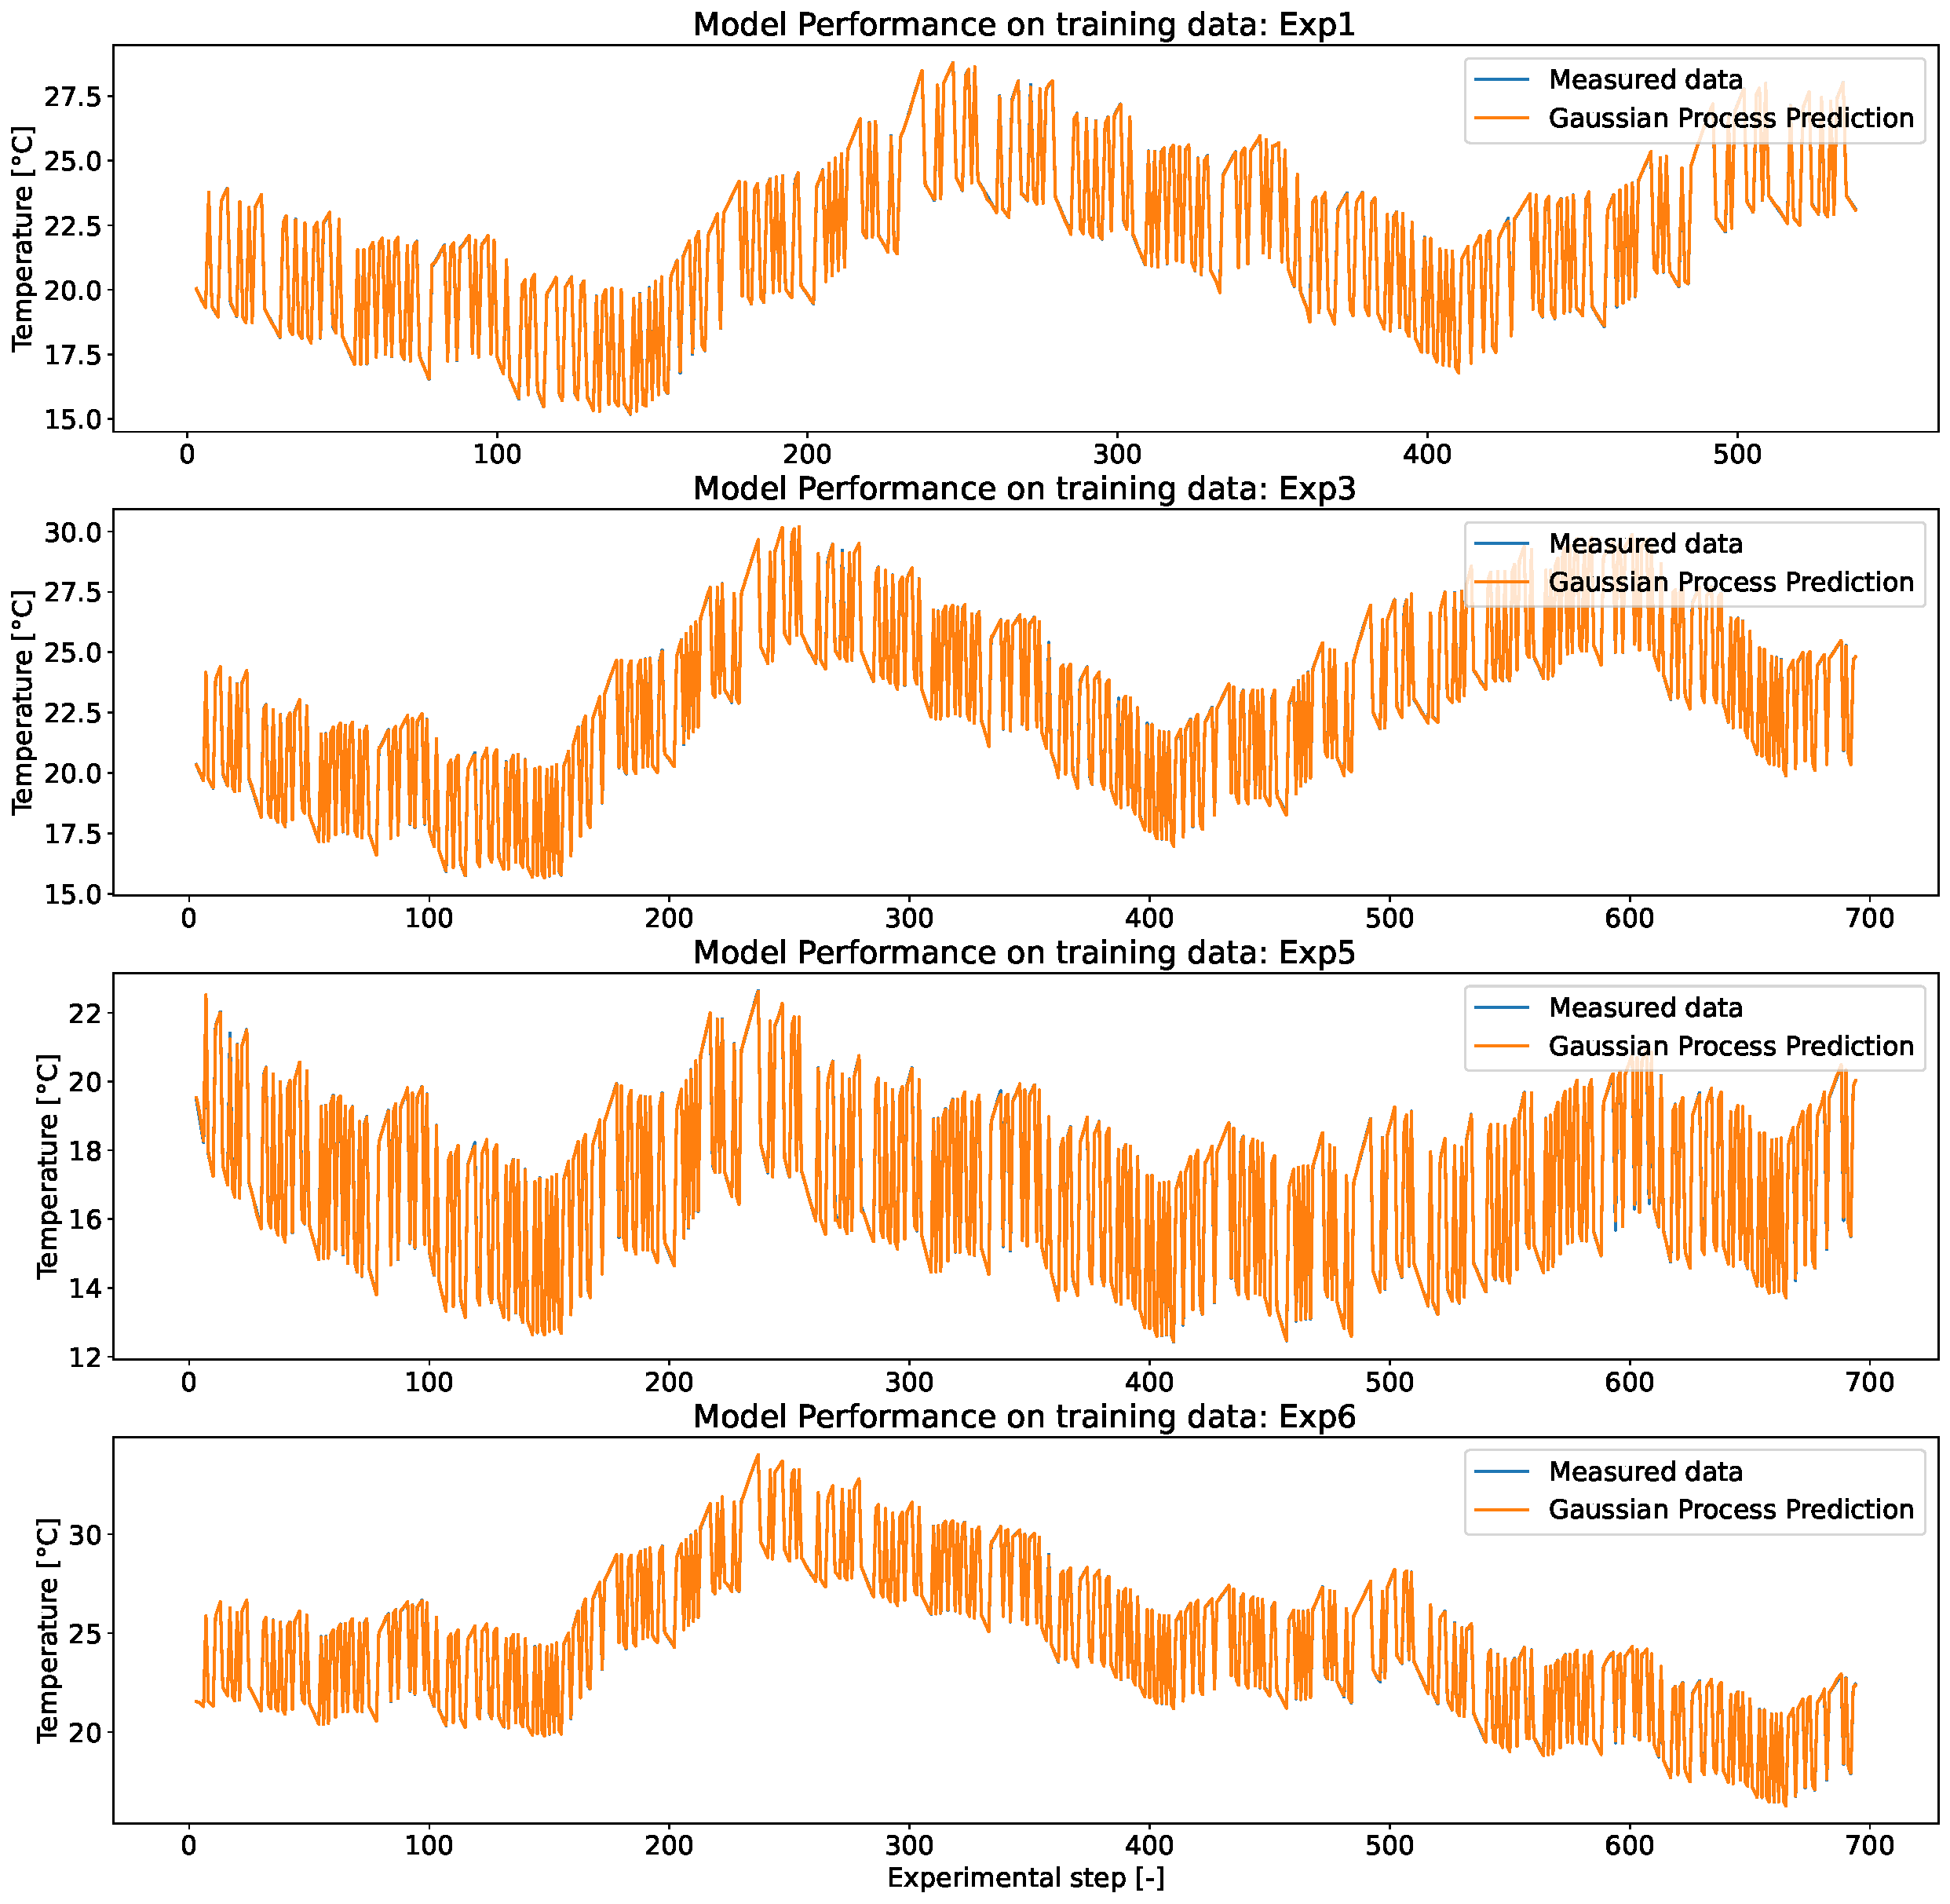
\includegraphics[width = \textwidth]{Plots/GP_213_training_performance.pdf}
    \caption{}
    \label{fig:GP_213_train_validation}
\end{figure}

\begin{figure}[ht]
    \centering
    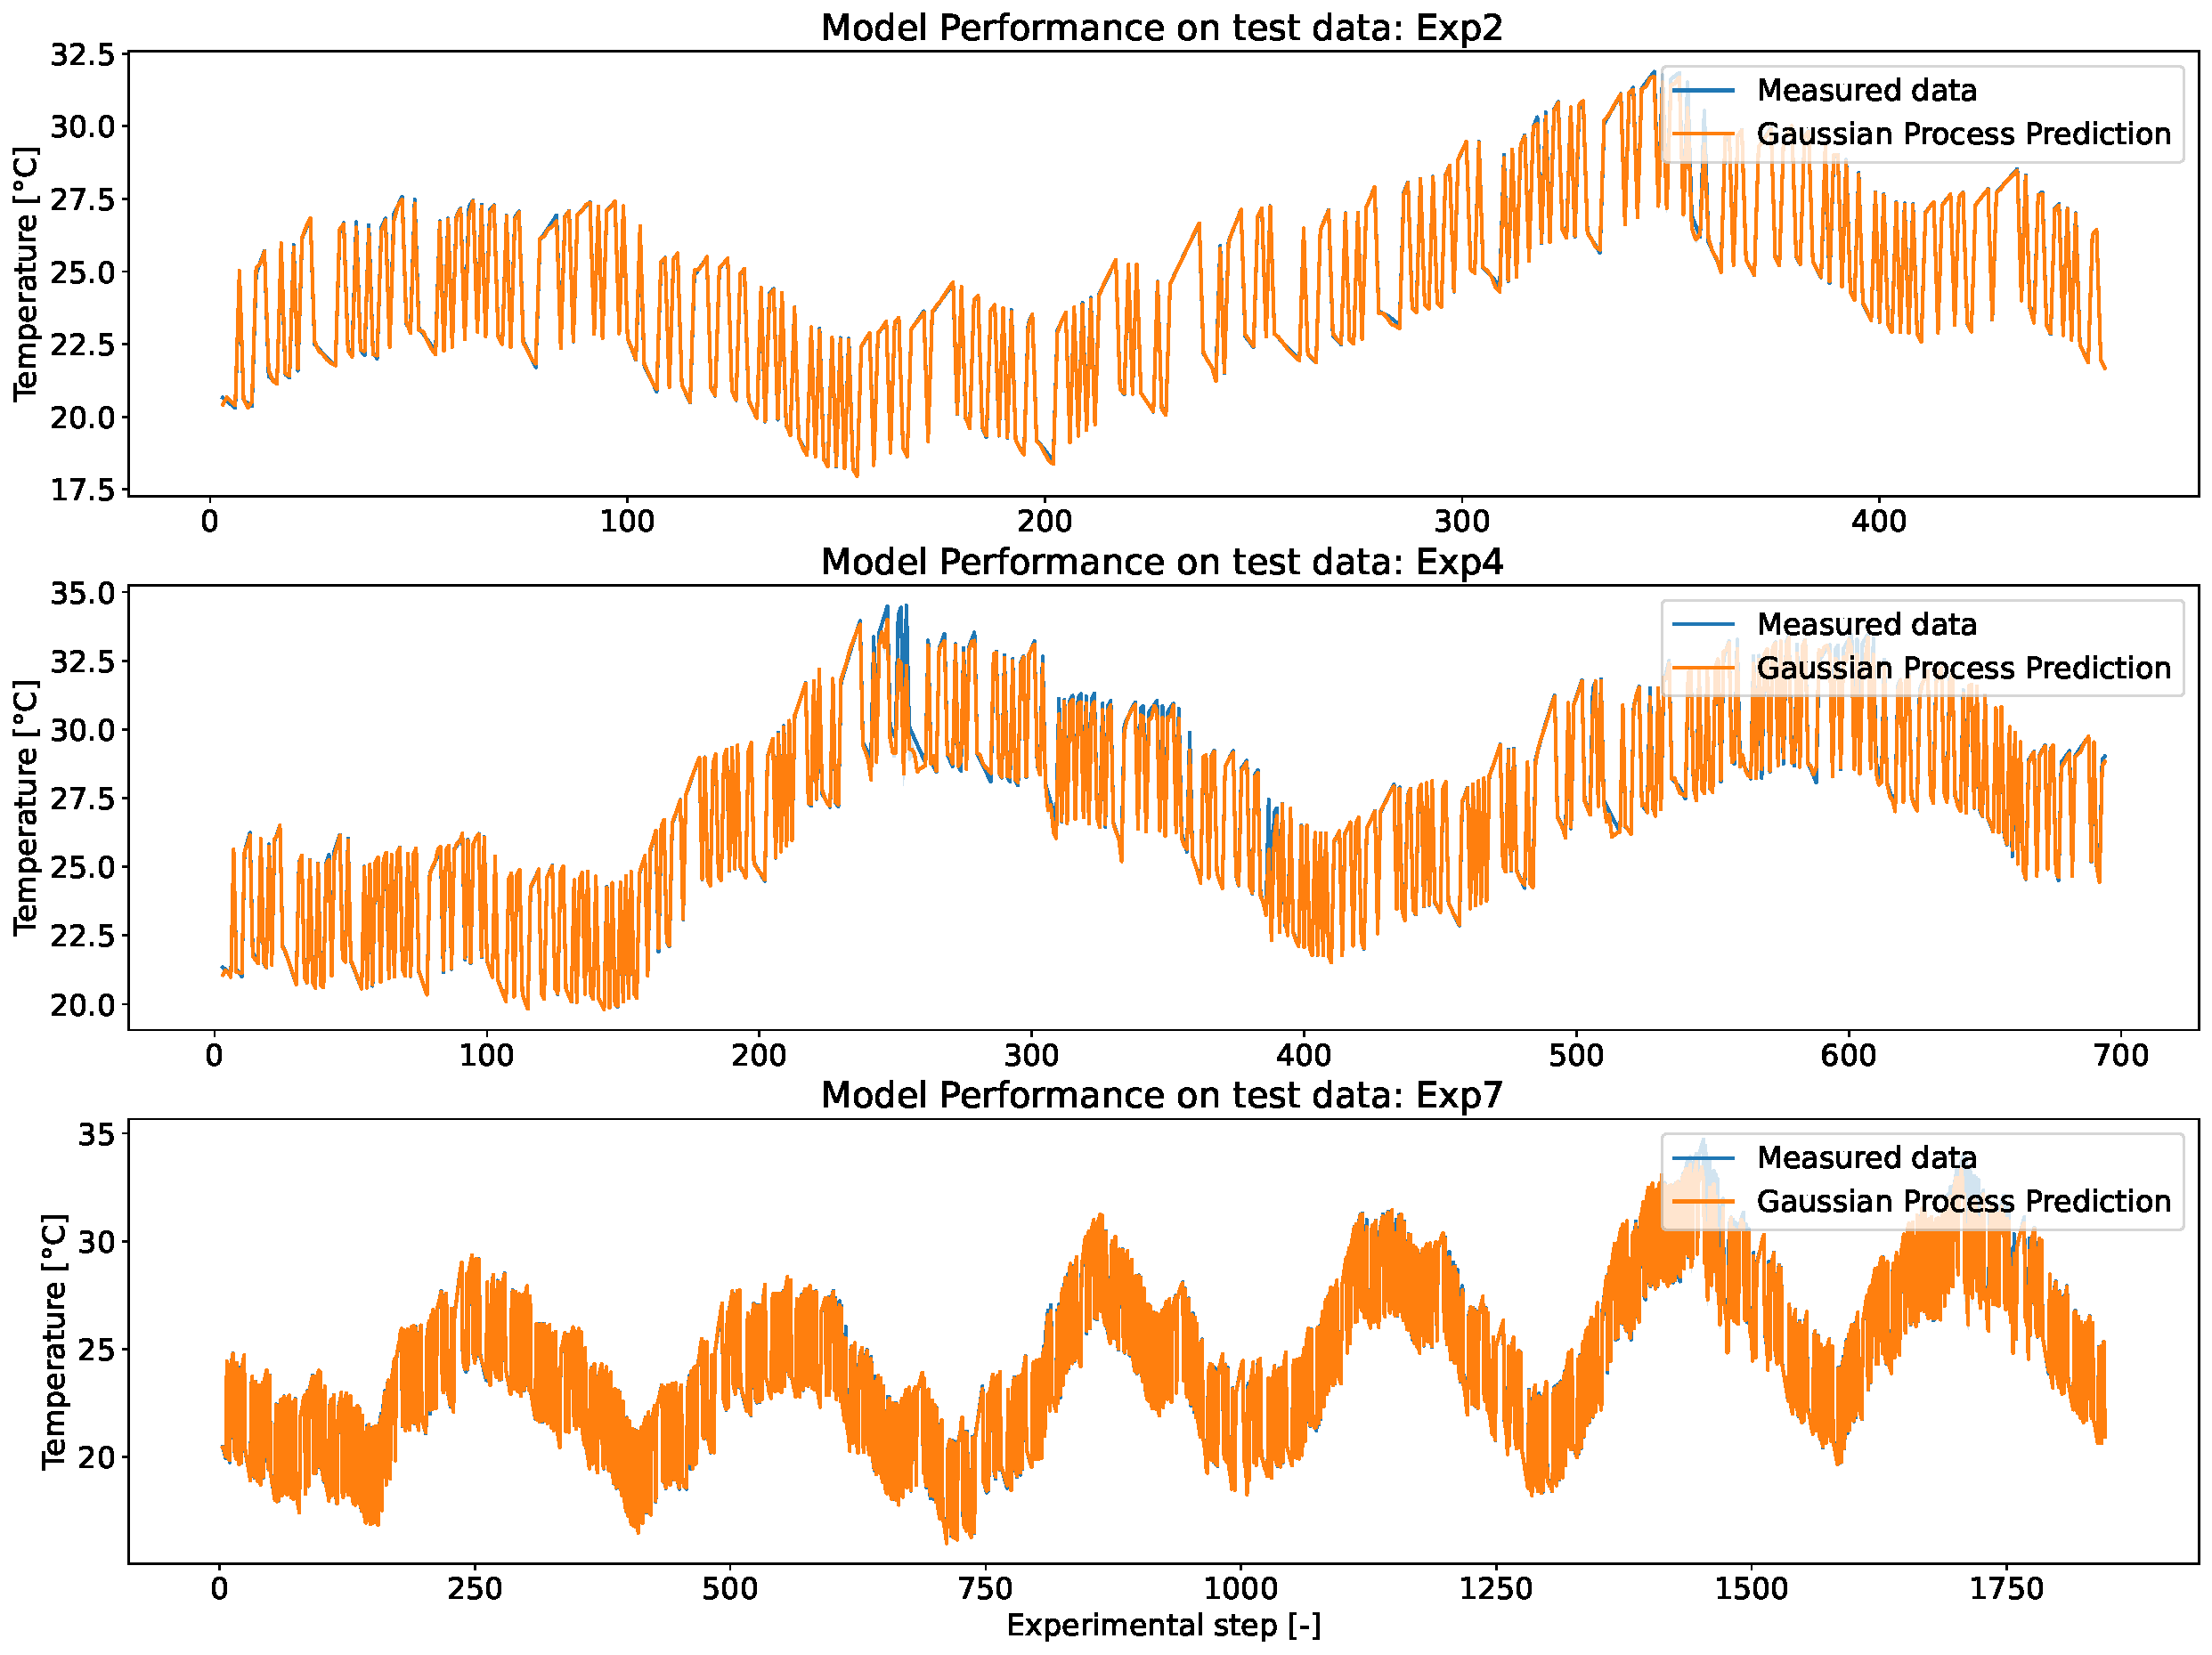
\includegraphics[width = \textwidth]{Plots/GP_213_test_performance.pdf}
    \caption{}
    \label{fig:GP_213_test_validation}
\end{figure}

\clearpage

\subsection{313}

\begin{figure}[ht]
    \centering
    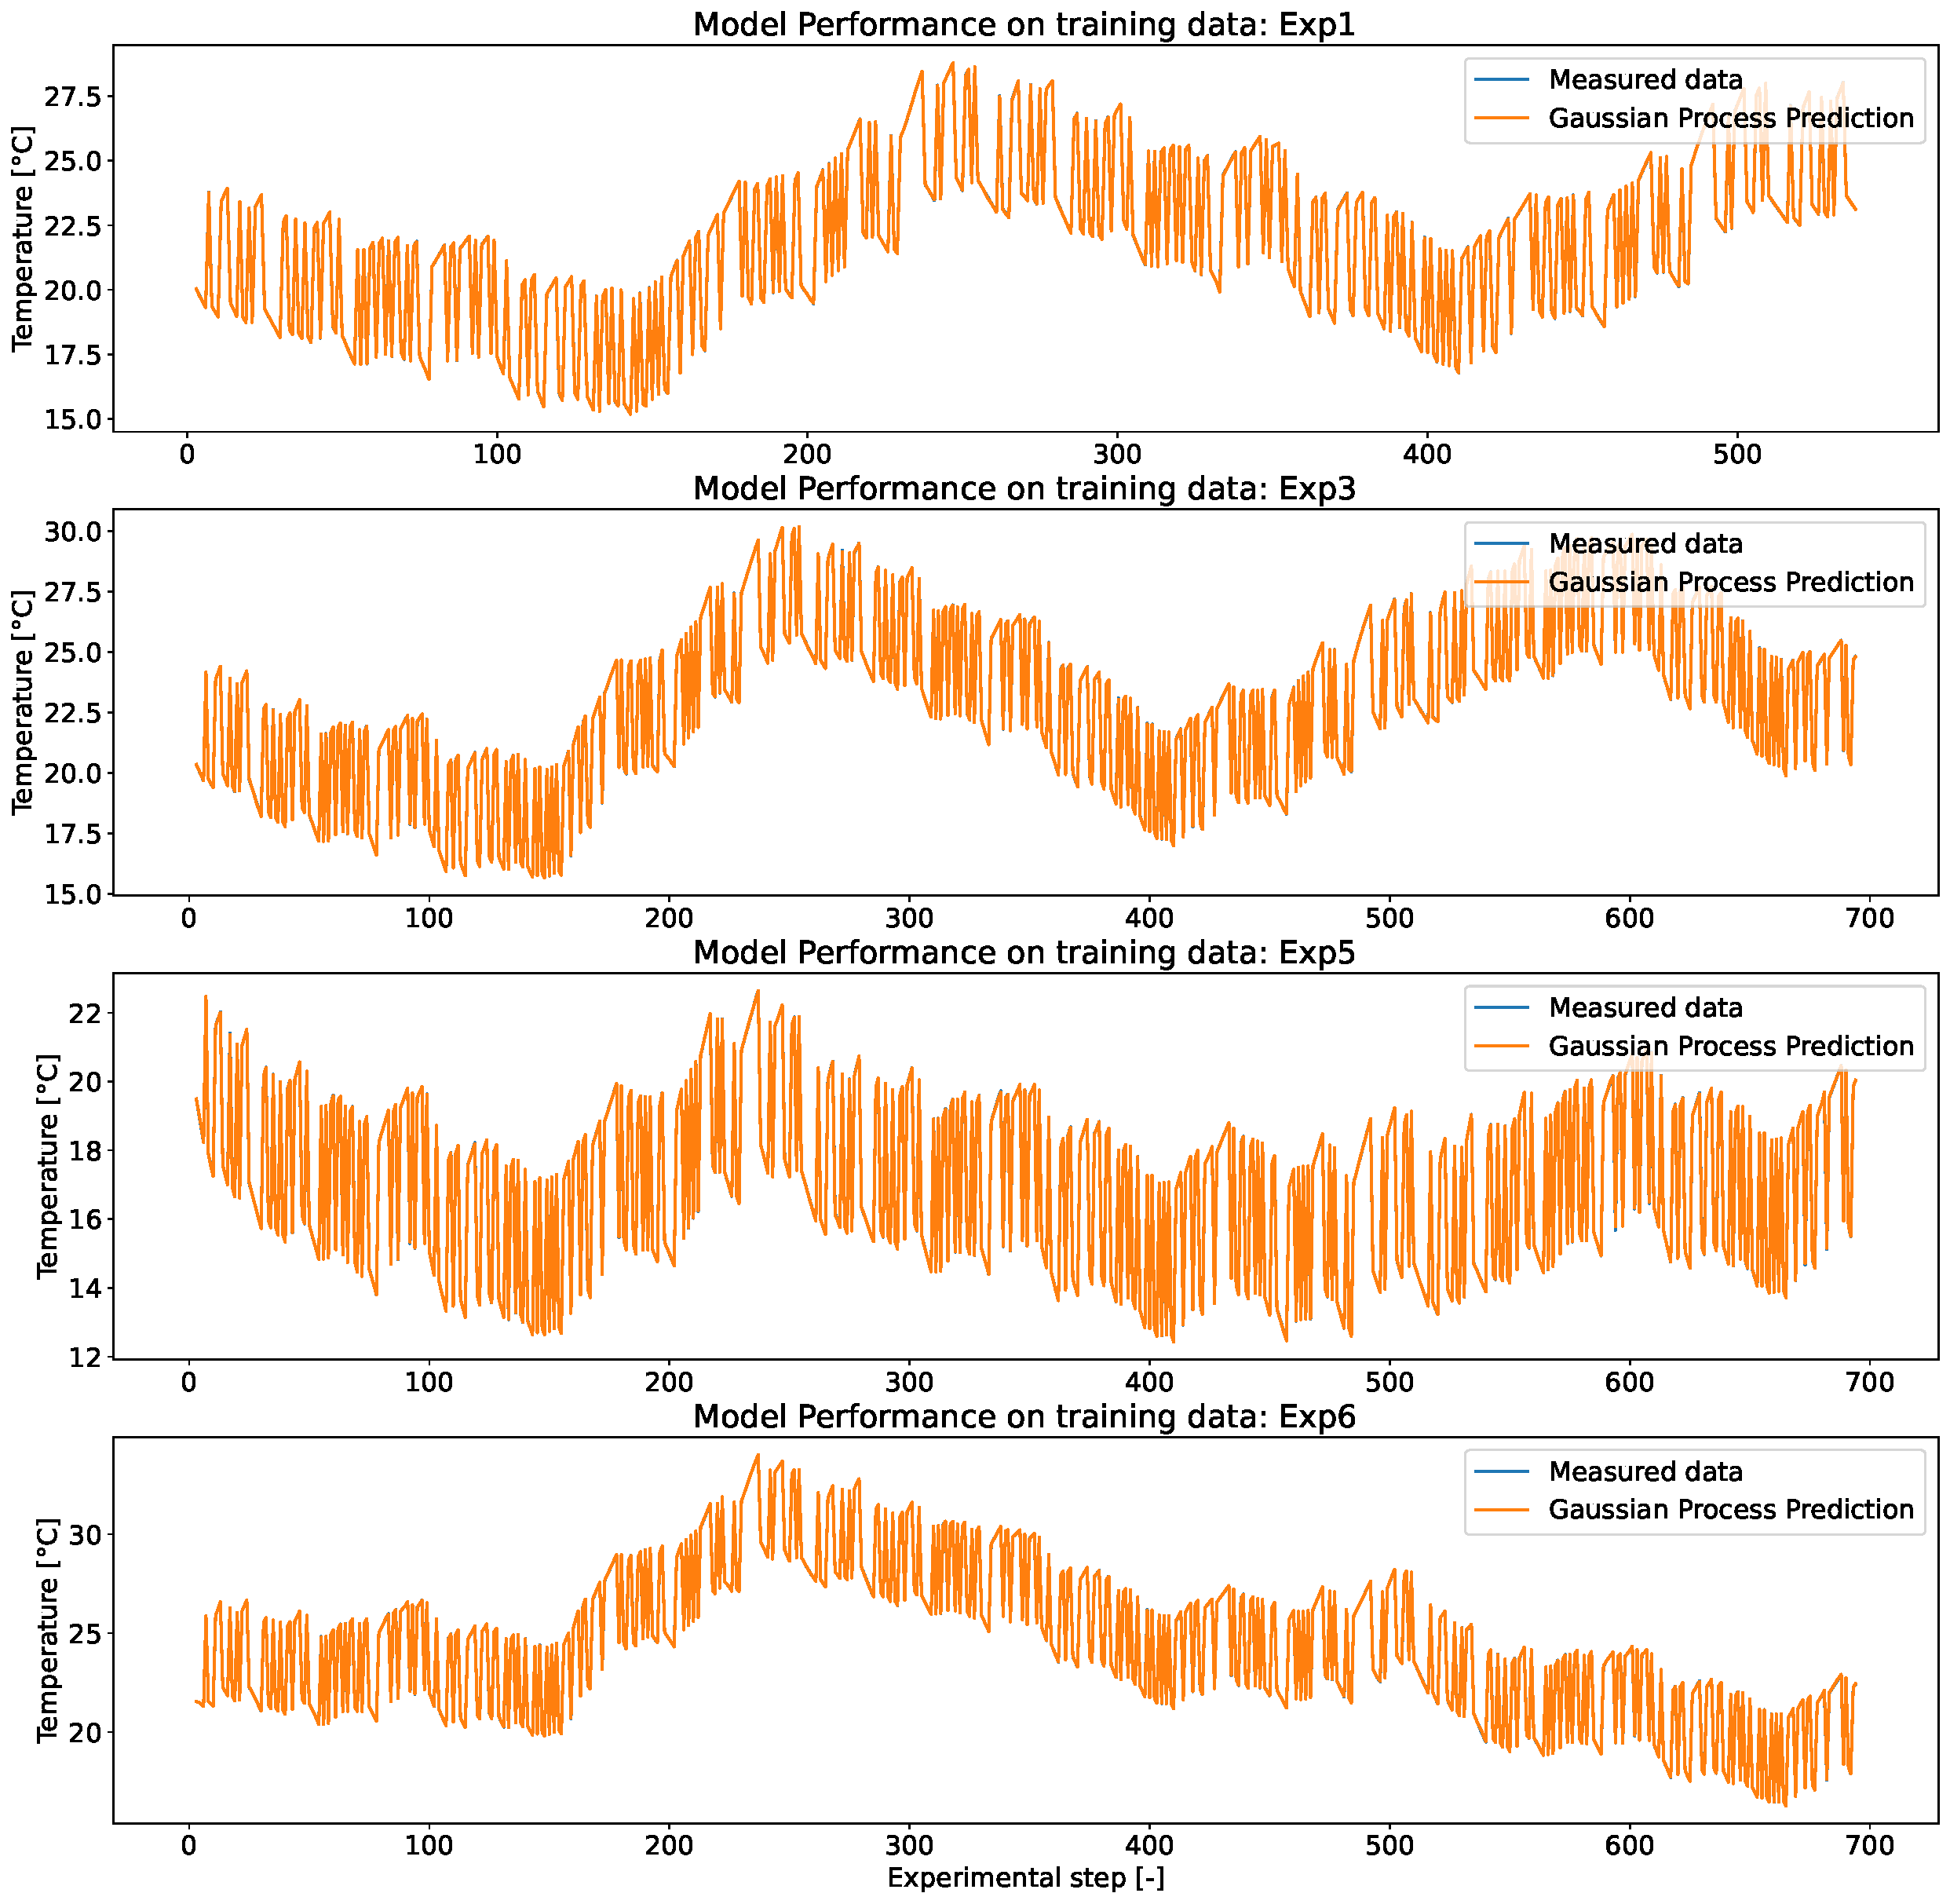
\includegraphics[width = \textwidth]{Plots/GP_313_training_performance.pdf}
    \caption{}
    \label{fig:GP_313_train_validation}
\end{figure}

\begin{figure}[ht]
    \centering
    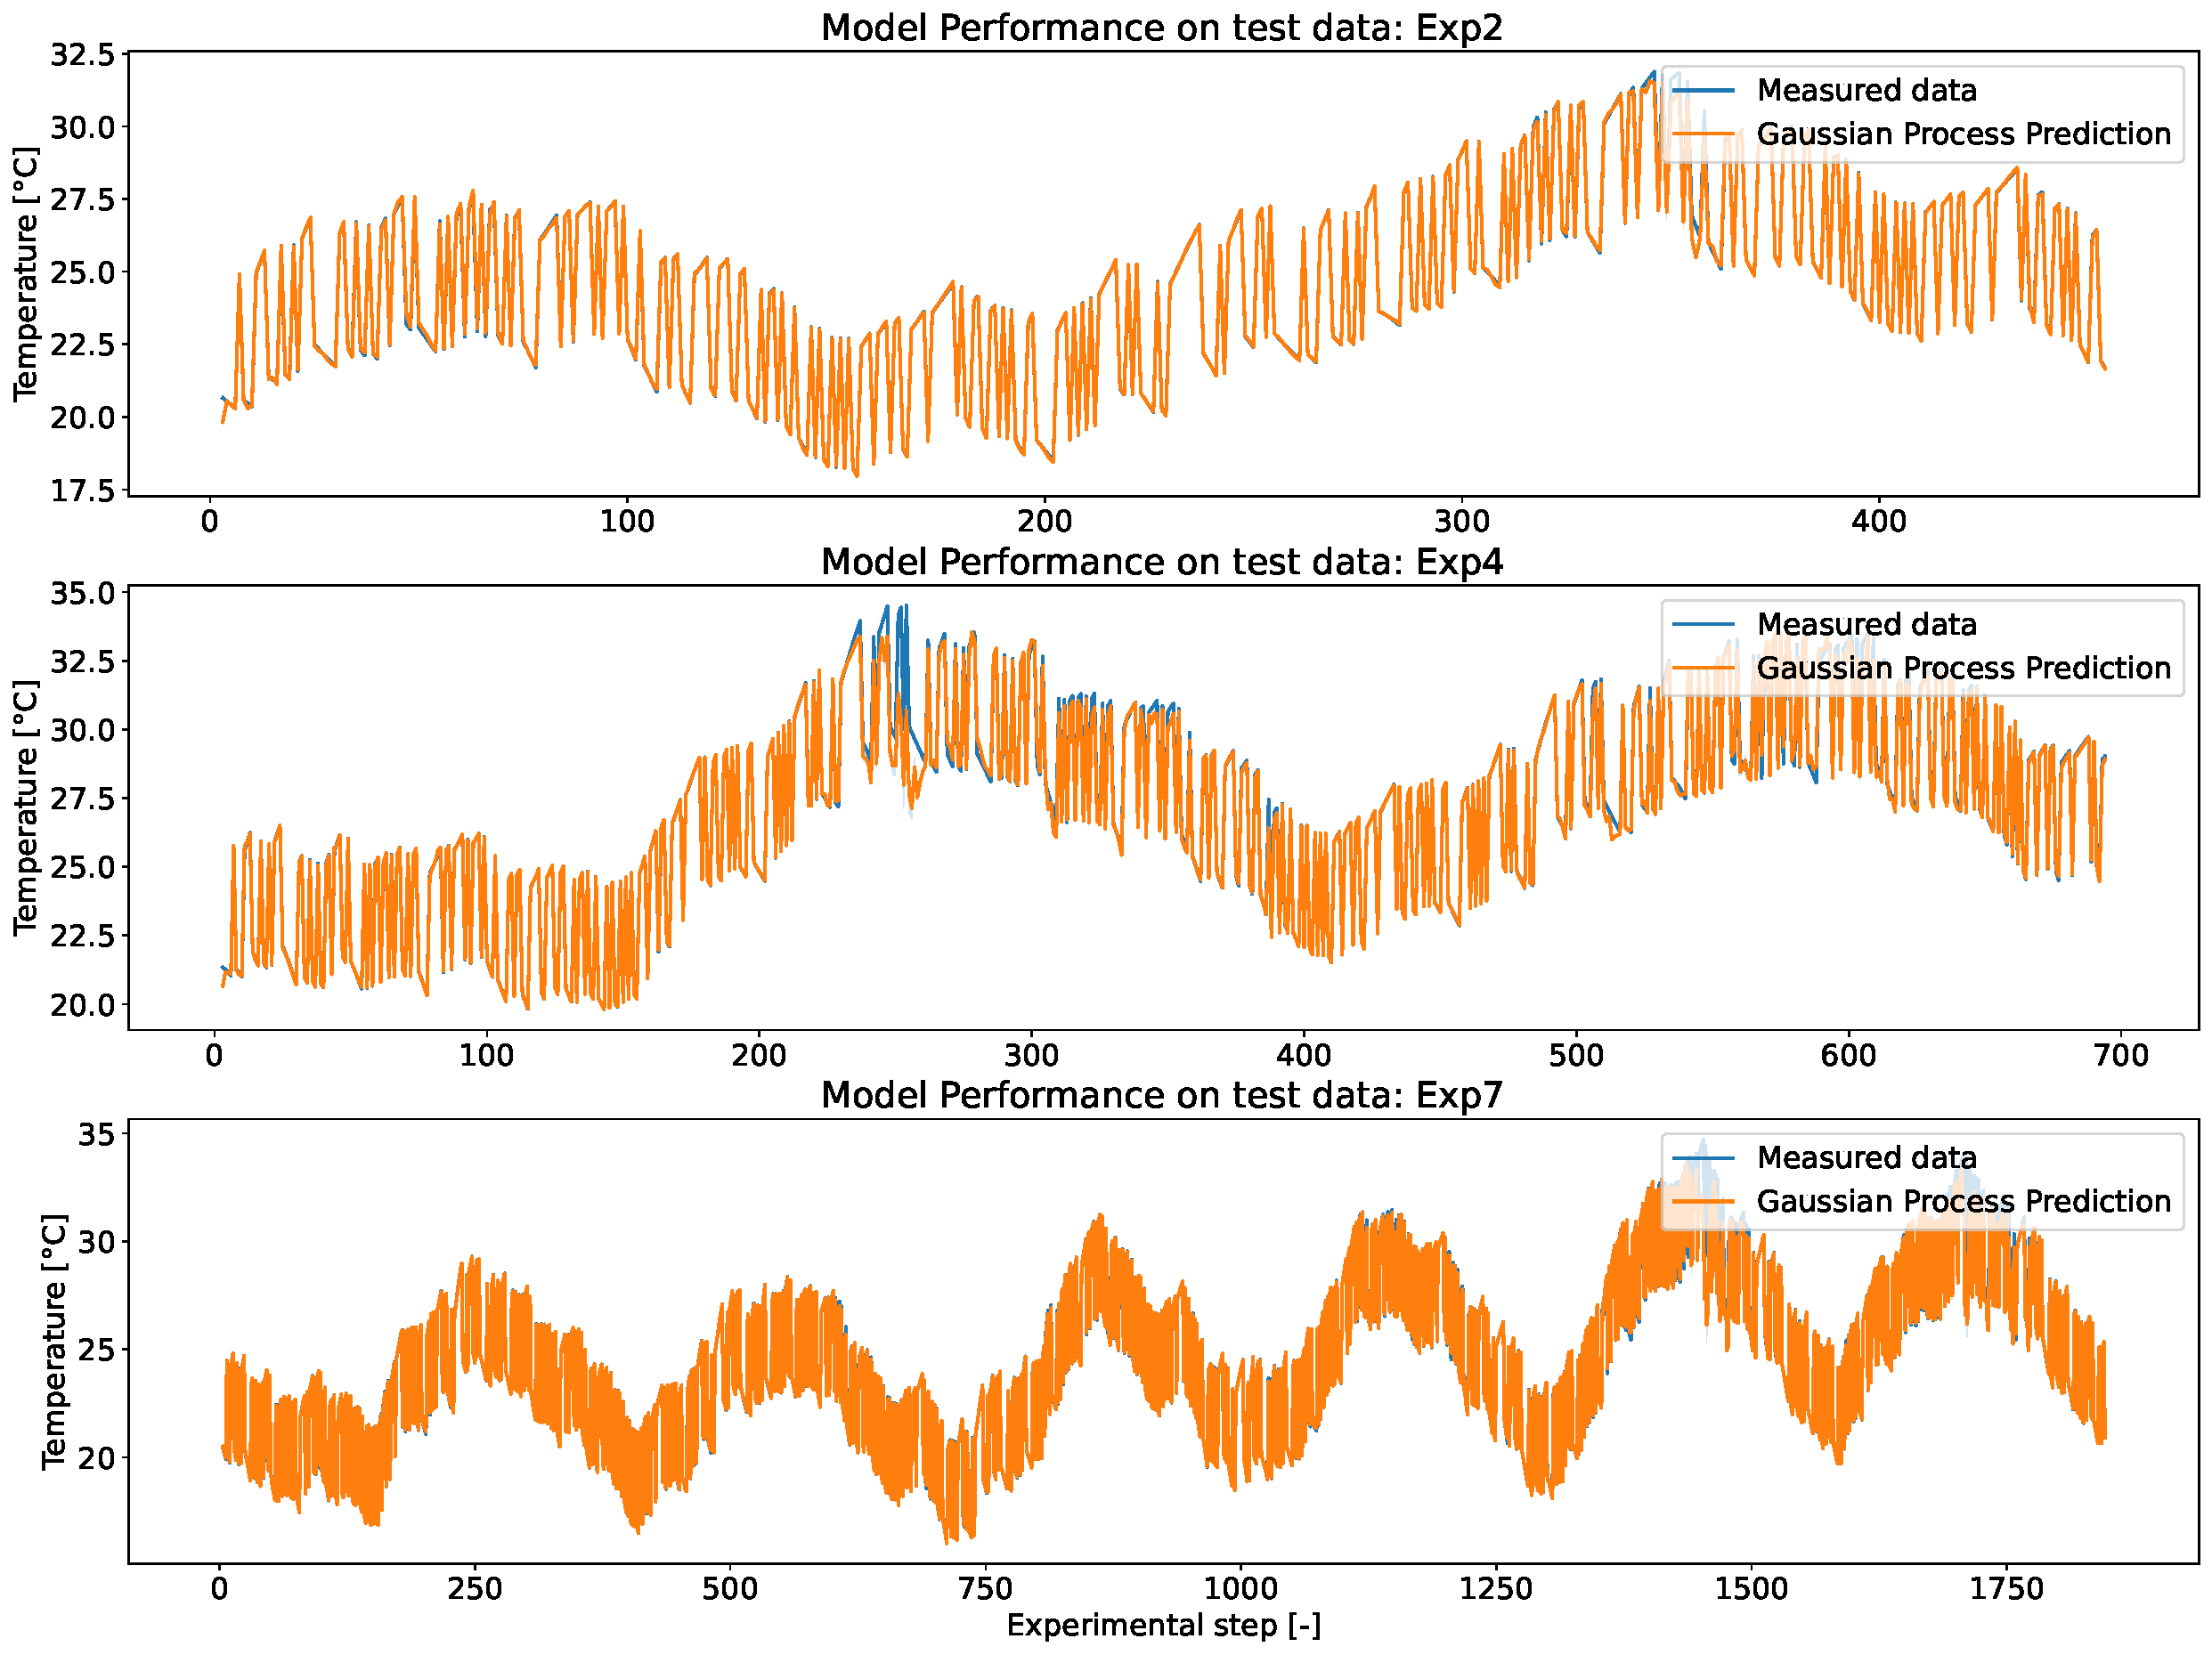
\includegraphics[width = \textwidth]{Plots/GP_313_test_performance.pdf}
    \caption{}
    \label{fig:GP_313_test_validation}
\end{figure}

\clearpage

\section{SVGP hyperparameters evolution}\label{anx:hyperparams_evol}

\begin{figure}[ht]
    \centering
    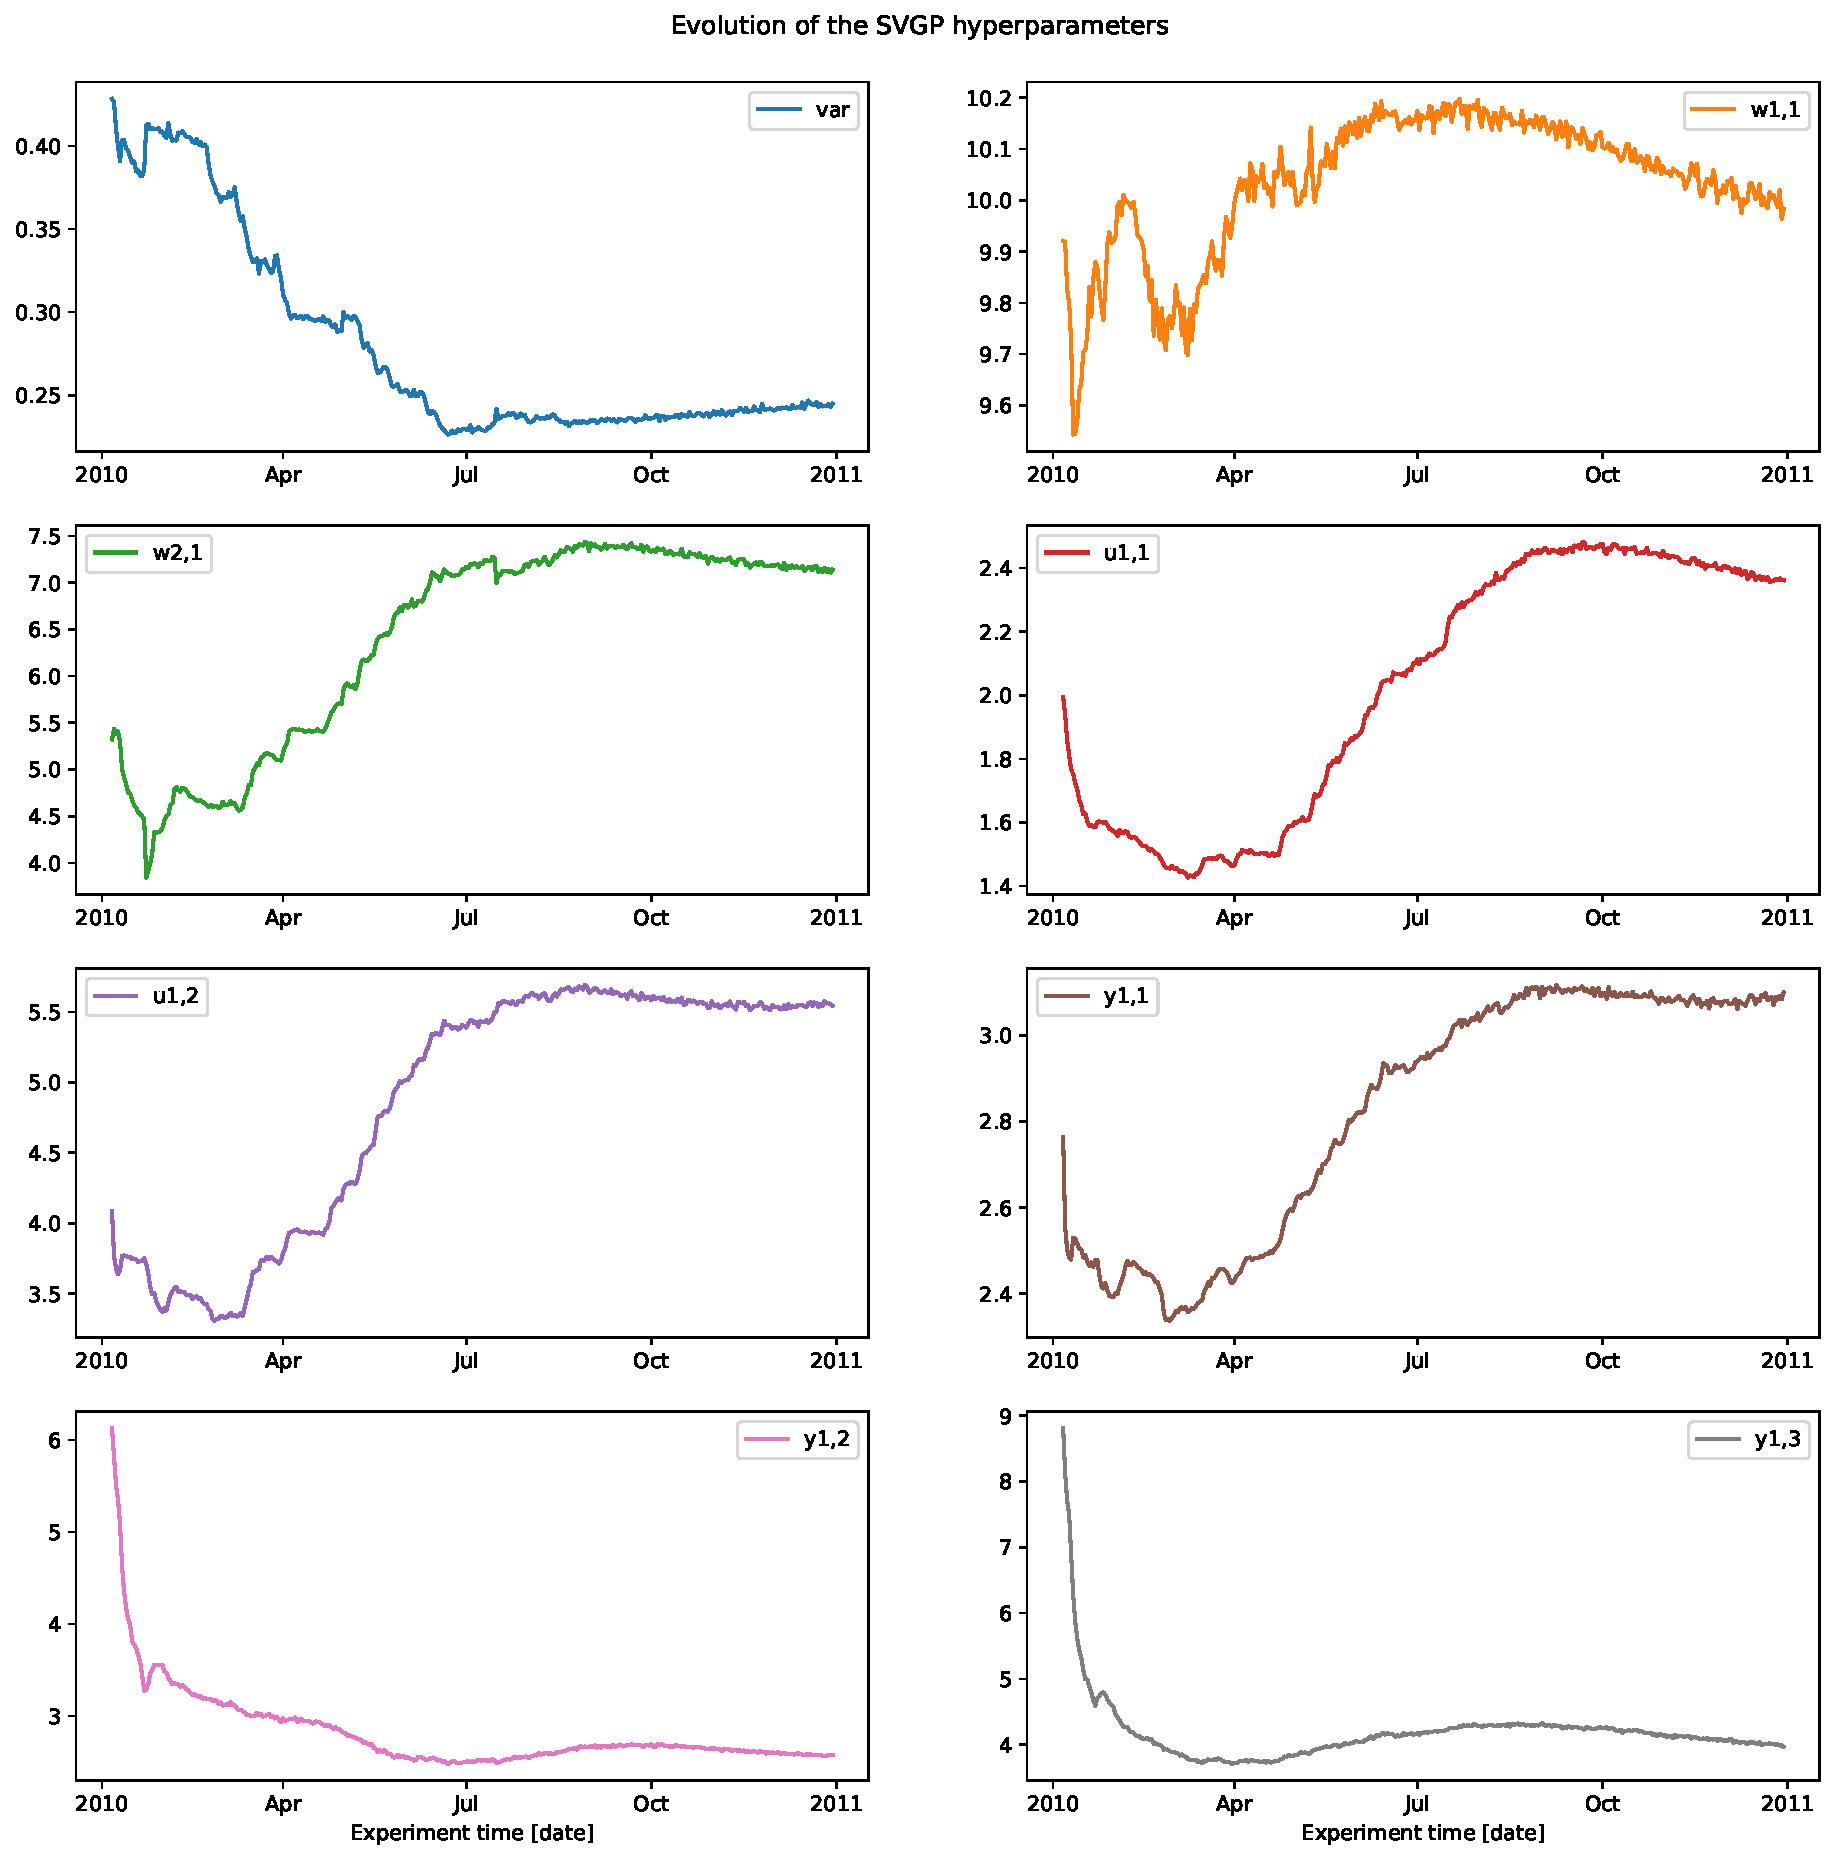
\includegraphics[width =
    \textwidth]{Plots/1_SVGP_480pts_inf_window_12_averageYear_evol_hyperparameters.pdf}
    \caption{Evolution of SVGP hyperparameters}
    \label{fig:SVGP_evol_hyperparameters}
\end{figure}


\end{document}
